
%------------- %   Document ma�tre   %------------- %


% % % % % % % % % % % % % % % % % % % % % % % % % % %
%													%
%   		Protocoles du SNO Tourbi�res			%
%													%
% % % % % % % % % % % % % % % % % % % % % % % % % % %


% % % % % %   AIDES   % % % % % %

%http://fr.wikibooks.org/wiki/LaTeX/Gestion_des_gros_documents


% % % % % %   Pr�ambule   % % % % % %

% Appel classe du document %
\documentclass[12pt,a4paper]{report}
% Appel du pr�ambule %

%--------------- %   Pr�ambule   %--------------- %

\usepackage[T1]{fontenc}
\usepackage[latin1]{inputenc}
\usepackage[frenchb]{babel}
\usepackage{amsmath}
\usepackage{amsfonts}
\usepackage{amssymb}
\usepackage{lscape}
\usepackage{graphicx}
\usepackage{url}
\usepackage{hyperref}
\usepackage{import}
%\usepackage{pgfplotstable}%pour importer les tables en csv
%\usepackage{csvsimple}%pour importer les tables en csv
\graphicspath{{Fig/}}
\author{S�bastien Gogo}
%\usepackage[top=2cm, bottom=2cm, left=2cm, right=2cm]{geometry}
%\title{Protocoles d'acquisition et de traitement des variables\newline \newline SNO Tourbi�res}
\setlength{\parindent}{0cm}
\setlength{\parskip}{1ex plus 0.5ex minus 0.2ex}
\newcommand{\hsp}{\hspace{20pt}}
\newcommand{\HRule}{\rule{\linewidth}{0.5mm}}
\usepackage{afterpage}
\newcommand\blankpage{%
    \null
    \thispagestyle{empty}%
    \addtocounter{page}{-1}%
    \newpage}

\usepackage{vhistory}


% Commandes de page et de titre %
%\title{SNO Tourbi�res - Protocoles d'acquisition et de traitement des mesures}
%\author{S�bastien Gogo}
%\maketitle
%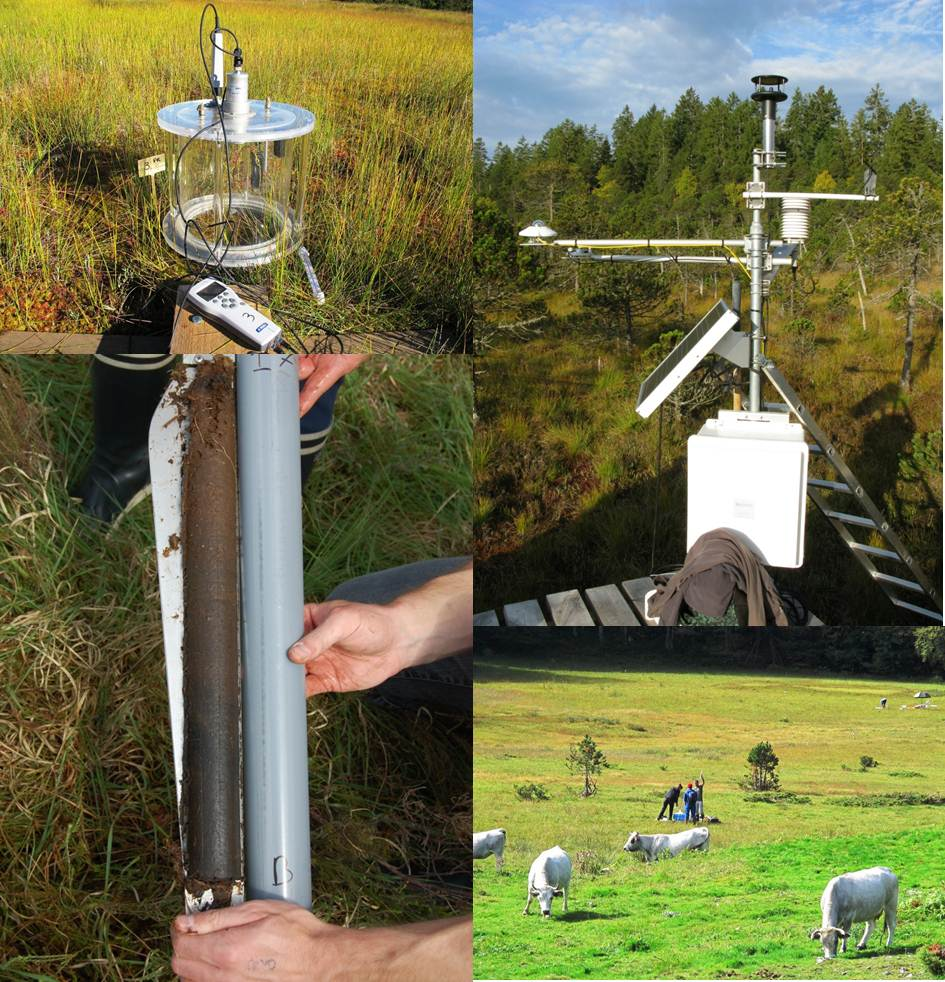
\includegraphics[width=14cm]{couverture.jpg}


% % % % % %   Document   % % % % % %

\begin{document}
	% Start of the revision history table

\begin{titlepage}

\begin{center}

	% Upper part of the page. The '~' is needed because \\
	% only works if a paragraph has started.
	~\\[-3cm]
	
\includegraphics[scale=0.5]{logo}~\\[1.5cm]
	
\includegraphics[scale=0.5]{logo_Tourbieres}\\[1cm]
	%\textsc{\Large Camp de terrain en Auvergne - semestre 1}\\[1.5cm]

	% Title
	\HRule \\[0.4cm]
	{ \huge \bfseries Protocoles d'acquisition et de traitement des mesures\\[0.4cm] }
	\HRule \\[2cm]
	

    
    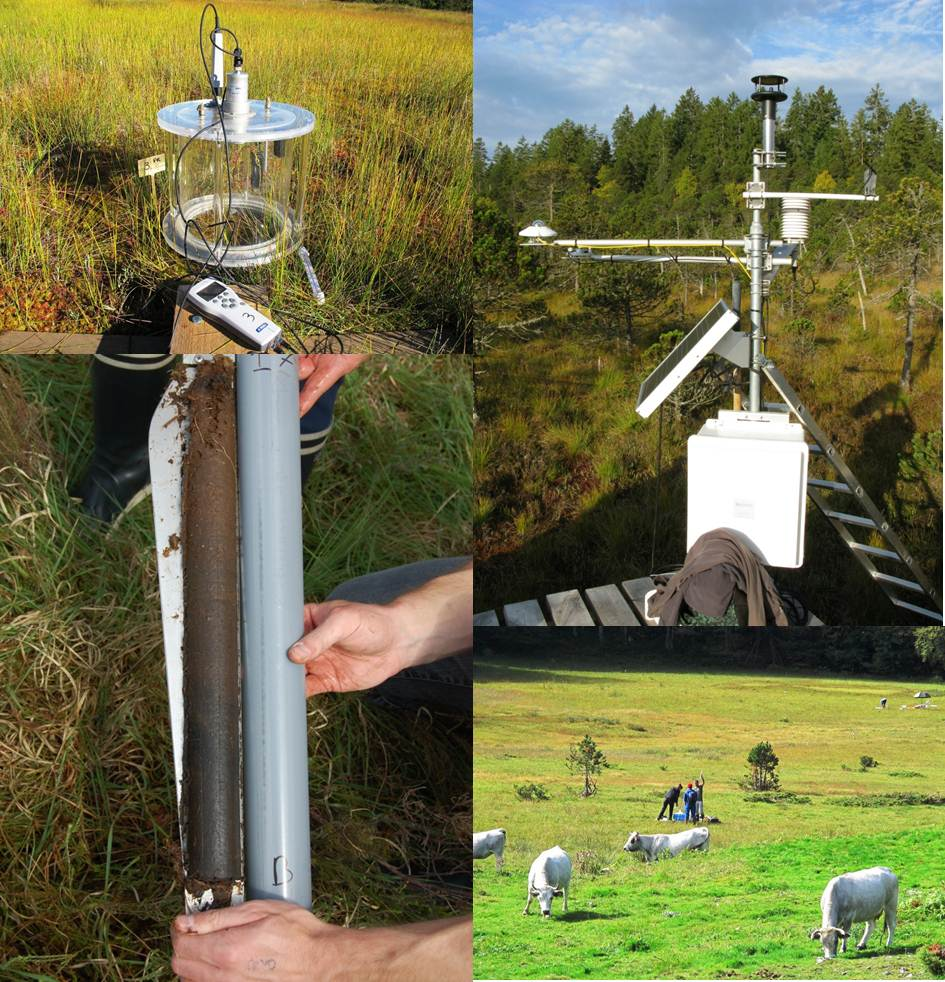
\includegraphics[scale=0.5]{couverture.jpg}
    \\[1cm]
    
	\text{\large S�bastien Gogo}\\[1cm]
    % Author and supervisor
    %\begin{minipage}{0.4\textwidth}
    %  \begin{flushleft} \large
    %   \emph{Encadrants :} M. Le \textsc{Tuteur}\\
    %  \end{flushleft}
    %\end{minipage}
    %\begin{minipage}{0.4\textwidth}
    %  \begin{flushright} \large
    %    \emph{Tuteur :} M. Le \textsc{Tuteur}\\
    %    \emph{Chef d'�quipe : } M. Chef \textsc{D?�quipe}
    %  \end{flushright}
    %\end{minipage}
    
    \text{16 janvier 2018}

    \vfill

	\begin{versionhistory}
		\vhEntry{1.0}{22.01.04}{JPW|KW}{created}
		\vhEntry{1.1}{23.01.04}{DP|JPW}{correction}
		\vhEntry{1.2}{03.02.04}{DP|JPW}{revised after review}
	\end{versionhistory}

    % Bottom of the page


  \end{center}

\end{titlepage}


	\afterpage{\blankpage}
	
	\tableofcontents
	\listoftables
	\listoffigures


\

		%--- CHAPITRE 1: Typologie et nomenclature des variables
		
%---------------------- %   Chapitre 1   %--------------------- %


% % % % % % % % % % % % % % % % % % % % % % % % % % % % % % % % %
%																%	
%		 SNO Tourbi�res - Typologie et nom des variables		%
%																%	
% % % % % % % % % % % % % % % % % % % % % % % % % % % % % % % % % 


%A REVOIR:
%1) tableau liste des variables
%2) ajouter tableau liste des variables facultatives



\chapter{Typologie des variables}

S.Gogo, M.-L. Toussaint, ...

\section{�l�ments de contexte et objectifs}

%JBP Pour les �l�ments de contextualisation, faire un bref point sur ICOS et rajouter �galement un point sur OZCAR.

Le Service National d'Observation des Tourbi�res (SNO Tourbi�res) a acquis, acqui�re et va acqu�rir un grand nombre de donn�es de diff�rents types, parfois de diff�rents formats (organisation des donn�es et format de fichier), dans des sites diff�rents, par des �quipes de recherches diff�rentes. Pour pouvoir g�n�rer des donn�es de qualit� � m�me de permettre un suivi sur le long terme coh�rent et une inter-comparaison entre site qui ait du sens, il est n�cessaire de ce mettre d'accord sur une liste de variable et sur la fa�on dont on les acqui�re et traite. Ceci passe par une harmonisation des noms et des formats de fichiers.

Les fichiers contenant les donn�es sont int�gr�s dans un syst�me d'information en environnement (SIE) pour les stocker, les traiter et permettre leur visualisation et leur t�l�chargement via une interface web pr�sente sur le site du SNO Tourbi�res\footnote{\url{http://www.sno-tourbieres.cnrs.fr/}}.

L'objectif de ce document est 1) de d�crire les types de variables et l'organisation des �quipements et des acquisitions manuelles pour ensuite 2) g�n�rer de mani�re coh�rente des noms de fichiers, de colonnes et de ligne commune � tous les types de donn�es pour rendre possible leur int�gration dans le SIE. Pour beaucoup de variables, nous suivront les recommandations provenant des protocoles de l'Integrated Carbon Observation System (ICOS\footnote{\url{http://www.europe-fluxdata.eu/icos/variables}}).

\newpage

\section{Cat�gorie et modes d'acquisition}

A ce jour un total autour de 42~variables cibles(Tableaux 1.1) sont ou seront suivies? dans le cadre du SNO Tourbi�re. Elles ont �t� regroup�es en 5 cat�gories:

\

		\begin{itemize}	
			\item \textbf{a - M�t�orologie, physique du sol}: M�t�o-sol
			
			\
			
			\item \textbf{b - Hydrologie hors profil "m�t�o-sol"}: Hydro/Carto 
			
			\
			
			\item \textbf{c - Flux de gaz � effet de serre}: GHG 
			
			
			\
			
			\item \textbf{d - Biog�o- physique et chimie}: Biog�o
			
			\
			
			\item \textbf{e - Biodiversit� et v�g�tation}: Bioveg
		\end{itemize}
		
\

%JBP d�finir gap-filling		
Pour les ateliers, les variables m�t�o-sol et GHG sont regroup�es car elles constituent un groupement coh�rent qui \textit{in fine} aboutiront aux calculs des flux et des bilans de carbone. Les donn�es m�t�o-sol serviront � comprendre les flux et � r�aliser le gap-filling des chroniques de flux. C'est dans les cat�gories m�t�o-sol, GHG et Bioveg o� se trouvent les variables n�cessaires � suivre pour �tre coh�rent avec ICOS. De ce fait, les cat�gories Hydro/Carto et Biog�o ont moins de contraintes que les 3 autres cat�gories.

\

%JBP Je te propose un tableau pour synth�tiser les diff�rents types de donn�es
Les donn�es correspondant aux variables des diff�rentes cat�gories sont acquises de mani�re diff�rentes (haute ou basse fr�quence d'acquisition, de mani�re r�guli�re ou irr�guli�re), sont inject�es sur le serveur du SNO Tourbi�res de mani�re diff�rentes (par t�l�communication ou manuellement) et ont un plus ou moins grand int�r�t relativement aux objectifs du SNO Tourbi�res. Le tableau \ref{priorite_donnees} �num�re par ordre de priorit�s d'int�gration dans le SIE ces types de donn�es et leur mode d'envoi sur le serveur. 

%\csvautotabular{priorisation_donnees.csv}

%JBP Rajout des r�f�rences de section
Certaines variables sont acquises par des capteurs plac�s sur le terrain et enregistr�es dans des stations d'acquisition. Ces stations d'acquisitions g�n�rent des fichiers qui contiennent les donn�es temporelles de plusieurs variables. Un maximum th�orique de 100 stations est pr�vue, mais concr�tement, le nombre de stations d'acquisition par site devrait se situer entre 10 et 20 par site. L'organisation des �quipements et des fichiers g�n�r�s par ces �quipement est d�velopp�e dans la section \ref{Organisation_equipement} et les variables acquises manuellement dans la section \ref{Organisation_campagne}. Les codes serviront ensuite � la nomenclature des fichiers g�n�r�s par chaque type de mesure.%JBP cette derni�re phrase n'est pas tr�s clair.

\newpage

\section{Les variables cibles obligatoires}

\subsection{D�finition et degr� d'�laboration}

% JBP Rajout des ref�rences de section
Les variables cibles sont les supports de l'interpr�tation du fonctionnement des syst�mes �tudi�s. A un degr� plus ou moins grand, toutes ces variables sont �labor�es (ayant subit au moins un calcul). Certaines de ces variables correspondent au signal de sortie d'un capteur comme par exemple la temp�rature du sol (juste un calcul machine). D'autres variables cibles vont �tre le fruit de nombreux calculs r�alis�s par la sonde et par l'expert. C'est le cas de la teneur en eau du sol. Un signal �lectrique est traduit en conductivit� �lectrique (calcul machine 1) qui sert � calculer la permittivit� �lectrique (calcul machine 2). Cette derni�re est utilis� dans une calibration "expert" avec des mesures manuelles pour obtenir la variables cible "teneur en eau". D'autres variables peuvent �tre calcul�es � partir de deux (ou plus) variables cibles. Le chemin r�alis� pour obtenir la variable cible � partir des donn�es obtenues sur le terrain est d�crit dans le chapitre \ref{v_meteosol}.\\
Le degr� d'�laboration d'une variable peut �tre cod� de la mani�re suivante :

		\begin{itemize}	
			\item Signal �lectrique brut du capteur: \textbf {b\_0}
			\item Calcul machine � partir du signal b\_0 : \textbf {b\_1}
			\item Calcul machine � partir du signal b\_1 : \textbf {b\_2}
			\item Calcul machine � partir du signal b\_n : \textbf {b\_n+1}
			\item Calcul expert � partir d'un signal b\_i et une calibration manuel :  \textbf {c\_0}
			\item Calcul expert � partir d'au moins 2 signaux b\_i (i>0) :  \textbf {c\_1}
		\end{itemize}


\subsection{Liste des variables cibles}
Les variables cibles suivies dans le cadre du SNO Tourbi�res de mani�res obligatoires sont � ce jour au nombre de 42 (tableau \ref{liste_variables}). Pour chaque variable cible, le code variable, la cat�gorie et le code de station/�quipement sont pr�cis�s. Ces derniers servent dans la d�signation des fichiers de donn�es. Les codes variables servent dans les ent�tes de colonnes. Les d�tails sur les types de capteurs, les fr�quence d'acquisition, la maintenance et les calculs sont donn�es au chapitre \ref{v_meteosol}.

Certaines variables sont facultatives. Le caract�re facultatif provient de la n�cessit� de mesurer une variable sp�cifique en fonction des caract�ristiques propre � un site. Pour l'instant, deux variables sont facultatives: la pr�cipitation sous forme de neige et l'azote totale dissous dans l'eau. Il est recommand� de pr�voir la hauteur de neige dans les sites les plus en altitude (Bernadouze et Frasne). 

\begin{table}
\begin{scriptsize}

\caption{Liste des variables cibles obligatoires .}
\label{liste_variables}

\

\begin{tabular}{l l l l l l}
	
			\hline
			\textbf{\#}&\textbf{Variable}&\textbf{Code}&\textbf{Cat�gorie}&\textbf{Station/�quipement}\\
			\hline
			1&Pression atmosph�rique&Pa&m�t�o-sol&\#1, 2, 3\\
			2&Pr�cipitation - pluie&P\_rain&m�t�o-sol&\#1, 2, 3\\	
			3&Densit� du flux de photon photosynth�tique&PPFD&m�t�o-sol&\#1, 2, 3\\
			4&Vitesse du vent 2D&WS&m�t�o-sol&\#1, 2, 3\\
			5&Direction du vent 2D&WD&m�t�o-sol&\#1, 2, 3\\
			6&Humidit� relative&RH&m�t�o-sol&\#1, 2, 3\\
			7&Temp�rature de l'air&Ta&m�t�o-sol&\#1, 2, 3\\	
			8&Temp�rature du sol&Ts&m�t�o-sol&\#1, 2, 3\\
			9&Teneur en eau du sol&SWC&m�t�o-sol&\#1, 2, 3\\
			10&Flux de chaleur dans le sol&G&m�t�o-sol&\#1, 2, 3\\
			11&Niveau de la nappe d'eau dans le sol (empreinte EC)&GWL&m�t�o-sol&\#1, 2, 3\\
			12&Rayonnement, longueurs d'ondes courtes entrantes&SWin&m�t�o-sol&\#1, 2, 3\\
			13&Rayonnement, longueurs d'ondes courtes sortantes&SWout&m�t�o-sol&\#1, 2, 3\\
			14&Rayonnement, longueurs d'ondes longues entrantes&LWin&m�t�o-sol&\#1, 2, 3\\
			15&Rayonnement, longueur d'ondes longues sortantes&LWout&m�t�o-sol&\#1, 2, 3\\
			16&Flux de H$_2$O par eddy covariance&FH2O&GHG&\#4\\
			17&Flux de CO$_2$ par eddy covariance&FCO2&GHG&\#4\\
			18&Flux de CH$_4$ par eddy covariance&FCH4&GHG&\#4\\
			19&Vitesse du vent 3D - composante horizontale&WSx&GHG&\#4\\
			20&Vitesse du vent 3D - composante lat�rale&WSy&GHG&\#4\\
			21&Vitesse du vent 3D - composante verticale&WSz&GHG&\#4\\
			22&Direction du vent 3D - x&WDx&GHG&\#4\\
			23&Direction du vent 3D - y&WDy&GHG&\#4\\
			24&Direction du vent 3D - z&WDz&GHG&\#4\\
			25&Flux de carbone organique dissous � l'�xutoire&FDOC&biog�ochimie&\#5\\	
			26&Flux de carbone organique particulaire � l'�xutoire&FPOC&biog�ochimie&\#5\\
			27&Conductivit� � l'�xutoire&Cond&biog�ochimie&\#5\\	
			28&Niveau de la nappe d'eau hors profil "m�t�o-sol"&GWL&hydro-carto&\#6 � 15\\
			29&D�bit � l'�xutoire &Q&hydro-carto&\#16 � 20\\
			30&Echange Net de l'Ecosyst�me - mesure chambre&NEEc&GHG&\#101 � 105\\
			31&Respiration de l'Ecosyst�me - mesure chambre&REc&GHG&\#101 � 105\\
			32&Production primaire brute - mesure chambre&GPPc&GHG&\#101 � 105\\
			33&Flux de  CH$_4$&FCH4c&GHG&\#106\\
			34&Temp�rature du sol manuelle&Tsm&GHG&\#107\\
			35&Teneur en eau du sol, manuelle&SWCm&GHG&\#108\\	
			36&Leaf Area Index&LAIm&GHG&\#109\\
			37&Carbone organique dissous, manuel&DOCm&biog�ochimie&\#110\\
			38&Carbone organique particulaire, manuel&POCm&biog�ochimie&\#111\\
			39&pH, manuel&pHm&biog�ochimie&\#112\\
			40&Conductivit�, manuel&Condm&biog�ochimie&\#112\\
			41&Niveau pi�zom�trique, manuel&GWLm&hydro-carto&\#113\\
			42&D�bit � l'�xutoire, manuel&Qm&hydro-carto&\#112\\		
			\hline
	
\end{tabular}
\end{scriptsize}
\end{table}



%\caption{Liste des variables facultatives acquises dans le
%cadre du SNO Tourbi�res.}
%\label{Table 2.}

\

%\begin{tabular}{l l l l l l}
	
		%	\hline
		%	\textbf{\#}&\textbf{Variable}&\textbf{Code}&\textbf{Cat�gorie}&\textbf{Transmission}\\
		%	\hline
		%	60&Pr�cipitation - neige&b&m�t�o-sol&#1, 2, 3\\
		%	\hline
	
%\end{tabular}
%\end{scriptsize}
%\end{table}

\section{Organisation des �quipements d'acquisition automatique}\label{Organisation_equipement}%JBP proposer �galement un tableau pour synth�tiser les codes de stations

Les donn�es acquises r�guli�rement et � haute fr�quence par des capteurs \textit{in situ} sont enregistr�es dans 4 types de station d'acquisition : i) m�t�o-sol (stations Campbell), ii) Eddy Covariance (station LICOR), iii) fluorescence de la mati�re organique dissoute (Fluorescence of Dissolved Organic Matter, FDOM - station Schnegg ou Xylem), iv) sondes pi�zom�triques hors profil "m�t�o-sol" (OTT, Diver, Campbell).

\subsection{Stations m�t�o-sol}
Sur chaque site du r�seau, il y aura 2 (minimum) voire 3 stations d'acquisition pour les variables m�t�o-sol: 

\

		\begin{itemize}
			\item station \textbf{\#001} = station m�t�o "classique" + physique du sol,
			
			\
			
			\item station \textbf{\#002} = station physique du sol.
				
			\
			
			\item station \textbf{\#003} = station physique du sol.
		\end{itemize}

\
%JBP ce point pourra �tre d�fini dans l'introduction car pour le moment, le lecteur n'a aucune id�e de ce que repr�sente les sites de niveau 2.
Nous adoptons le nombre et la nomenclature des variables recommand�es par ICOS pour les sites de niveau 2. De mani�re minimale, deux profils complets seront install�s.

La station m�t�o "classique" enregistre les variables permettant de caract�riser le site et de calculer l'�vapo-transpiration potentielle: temp�rature de l'air, pression atmosph�rique, pr�cipitation, vitesse et direction du vent, humidit� relative de l'air et rayonnement.

%JBP rajouter des liens \ref{}
Dans les variables m�t�o-sol, il y a le niveau de la nappe d'eau dans l'empreinte de la tour � flux. Les sondes qui mesurent ces niveaux d'eau (branch�es sur les stations Campbell) ne sont pas consid�r�es dans le paragraphe 1.10 concernant les variables \og{} hydro\fg{}. Les sondes consid�r�es dans le paragraphe 1.10 correspondent aux sondes de mesures de niveau d'eau se situant � l'ext�rieur des profils "m�t�o-sol".


\subsection{Station Eddy Covariance (EC)}
Une station d'acquisition est pr�sente au niveau du m�t EC pour enregistrer toutes les variables n�cessaires aux calculs des flux de CO$_2$, CH$_4$ et H$_2$O, et la direction et vitesse du vent en 3D:

\

		\begin{itemize}	
			\item station \textbf{\#004} = station d'acquisition EC.	
		\end{itemize}

\
%JBP Rajouter le lien vers le propotcole d'acquisition des donn�es EC
Le calcul des flux est r�alis� � la fr�quence d'un flux toutes les 30 minutes. Ceci n�cessite l'acquisition de tous les param�tres � une fr�quence de 20Hz (cf protocole sur l'EC pour tous les d�tails). La station d'acquisition Licor calcule un flux "imm�diat" chaque 30 minutes qui servira � v�rifier que l'appareil fonctionne bien. Cependant, il s'agit juste d'une valeur indicative puisque la vraie valeur de flux sera calcul�e par les experts de cette variable (avec le support des coll�gues d'ICOS).


\subsection{Fluorim�tre de terrain � l'exutoire}
%JBP Correspond aux groupes de variable hydro-carto? A pr�ciser
Un fluorim�tre avec un syst�me d'acquisition est pr�sent au niveau de l'exutoire principal de chaque site:

\

		\begin{itemize}	
			\item station \textbf{\#005} = station d'acquisition du fluorim�tre � l'exutoire.
		\end{itemize}
		
		
\subsection{Sondes pi�zom�trique hors profil "m�t�o-sol"}
Des sondes de mesure du niveau d'eau contenant leur syst�me autonome d'acquisition sont d�ploy�es � diff�rents endroits dans (de 6 � 15) et � l'exutoire (de 16 � 20) de chaque tourbi�re :

\

		\begin{itemize}	
			\item station \textbf{\#006} = sonde pi�zom�trique 1 dans la tourbi�re,
			
			\
			
			\item station \textbf{\#007} = sonde pi�zom�trique 2 dans la tourbi�re,
			
			\
			
			\item station \textbf{...}
			
			\
			
			\item station \textbf{\#015} = sonde pi�zom�trique 10 dans la tourbi�re,
			
			\
			
			\item station \textbf{\#016} = sonde pi�zom�trique 1 � l'�xutoire,
			
			\
			
			\item station \textbf{...}
			
			\
			
			\item station \textbf{\#020} = sonde pi�zom�trique 5 � l'�xutoire,	
		\end{itemize}
		
\


\subsection{Stations d'acquisitions suppl�mentaires}

Si un nouveau dispositif (e.g. mesures de concentration en carbone inorganique dissous � l'�xutoire), une station d'acquisition m�t�o-sol, eddy-covariance, fluorim�tre et/ou sonde pi�zom�trique sont ajout�s, ils prendront le num�ro suivant � partir de 21 jusqu'� 100: de 21 � 30 pour les stations m�t�o-sol, de 31 � 40 pour les tour EC, de 41 � 50 pour les fluorim�tres, de 51 � 70 pour les pi�zom�tres et de 71 � 100 pour tout appareil nouveau.

\newpage

\section{Organisation des campagnes d'acquisition manuelle}\label{Organisation_campagne}
Les variables acquises de mani�res manuelles sont regroup�es par �quipement de mesures. La liste des �quipements commence � 101.

\subsection{Mesure de flux par chambre d'accumulation}
Les �quipements utilis�s pour les mesures de flux de C en chambres ferm�es ont �t� choisies par les �quipes d'Orl�ans: Vaisala pour le CO$_2$ et Los Gatos pour le CH$_4$ (voir chapitre ? pour plus de d�tails). Les chambres peuvent �tre pos�es manuellement ou automatiquement, suivant les moyens disponibles. Les points de mesures sont au nombre de dix et doivent couvrir la variabilit� spatiale de la v�g�tation dans l'empreinte. Cependant, les mesures sont effectu�es par 5 (tirage au sort). Pour interpr�ter les flux, des variables explicatives sont enregistr�es : un profil de temp�rature du sol � proximit� de la mesure de flux, la teneur en eau des premiers centim�tres de tourbe et l'indice de surface des feuille (leaf area index ou LAI).

Dans le r�seau ICOS, les mesures de flux avec les chambres ne sont obligatoires que pour les sites de niveau 1. Dans le cadre du SNO Tourbi�res, nous avons pour objectif de tendre vers les recommandations pour les sites de niveau 2. Compte-tenu de l'importance de la connaissance de la variabilit� spatiale des flux dans la compr�hension du bilan � l'�chelle de l'�cosyst�me, nous essaierons tout de m�me de mettre en place dans tous les sites des mesures en chambre. Nous suivrons les recommandations ICOS puisqu'elles existent, mais nous autoriseront une certaine flexibilit�.

\

	\begin{itemize}	
			\item �quipement \textbf{\#101 � 105} = mat�riel Vaisala pour le CO$_2$,
			
			\
			
			\item �quipement \textbf{\#106} = mat�riel Los Gatos pour le CH$_4$,
			
			\
			
			\item �quipement \textbf{\#107} = sonde pour mesure de profils de temp�rature,
			
			\
			
			\item �quipement \textbf{\#108} = sonde teneur en eau,
			
			\
			
			\item �quipement \textbf{\#109} = LAI-m�tre.	
		\end{itemize}

\

Les �quipements de \#101 � 105 correspondent � 5 chambres manuelles ou automatiques. Chaque station produira un fichier avec l'ensemble des variables correspondant � son point de mesure. Si les mesures sont r�alis�es manuellement, une m�me chambre (la \#101) sera utilis�e pour tous les points de mesures et un seul fichier (...\_101\_...) sera g�n�r� avec les variables de tous les points de mesures.


		
\subsection{Chimie et physique de l'eau}

%JBP Rajouter \ref{}

Pour caract�riser les sites et compl�ter le bilan de C � l'�chelle de l'�cosyst�me, des analyses chimiques et physiques seront r�alis�es sur les eaux � l'exutoire et dans la tourbi�re (eau dans les pi�zom�tre).
%JBP Rajouter le point sur les variables obligatoires n'est pas clair, il est contradictoire avec ce qui est d�velopp� dans la section 1.13
Les �l�ments mesur�s sont: le carbone organique dissous (DOC, variable obligatoire), le carbone organique particulaire (POC, variable obligatoire) l'azote totale (TN, variable facultative). Ces variables sont mesur�es sur des �chantillons d'eau ramen�s au laboratoire (voir chapitre ? pour plus de d�tails). Pour le DOC et le TN, l'appareil de mesure est un DOC-m�tre (e.g. Shimadzu). Le POC correspond � la masse de C contenu dans les mati�res dont la taille est sup�rieure � 0.45~$�$m.
A chaque �chantillonnage � l'exutoire et dans la tourbi�re, le pH, la temp�rature et la conductivit� de la solution seront mesur�s avec des sondes multiparam�tres (e.g. WTW).

\

	\begin{itemize}	
			\item �quipement \textbf{\#110} = COT-m�tre%JBP(COT-m�tre ou DOC-m�tre??)
			
			\
			
			\item �quipement \textbf{\#111} = balance + analyseur �l�mentaire
			
			\
			
			\item �quipement \textbf{\#112} = sonde multiparam�tres	
	\end{itemize}
		
		
\subsection{D�bit � l'�xutoire}
Pour obtenir des mesures de d�bit � haute fr�quence, des mesures de niveau d'eau � l'�xutoire � haute fr�quence (stations de 016 � 020) sont coupl�es avec des mesures manuelles de d�bit. La m�thode utilis�e dans tous les sites est la m�thode du d�bit au sel (voir chapitre 4 pour plus de d�tails). Elle utilise un conductim�tre. Le d�bit est ensuite calcul� � partir des variations de conductim�trie en fonction du temps.

\

	\begin{itemize}	
			\item �quipement \textbf{\#112} = conductim�tre (sonde multiparam�tres)
	\end{itemize}

\subsection{Niveau d'eau}
Des mesures manuelles dans tous les pi�zom�tres �quip�s de sondes automatiques sont n�cessaires pour corriger les chroniques. Ces mesures sont r�alis�es avec une sonde manuelle ou avec un m�tre (� pr�ciser dans le m�tadonn�es).

\

	\begin{itemize}	
			\item �quipement \textbf{\#113} = sonde pi�zom�trique manuelle ou m�tre
	\end{itemize}

\subsection{Equipements suppl�mentaires}
Les mesures suppl�mentaires seront num�rot�es par type d'�quipement � partir de 114. Dans l'id�al, le choix et le d�but du monitoring d'une variable sur un site devrait �tre l'objet d'une discussion lors d'un comit� de pilotage. Si la variable est retenue, un num�ro sera attribu� � l'�quipement et les autres sites qui seront capables de suivre cette nouvelle variables devront reprendre le m�me num�ro d'�quipement. Exemple: si un responsable de site a envie (besoin) de mesurer sur un an (voire plus) les concentrations en azote inorganique (nitrate, nitrite, ammoniaque) � l'exutoire, et si le copil est d'accord pour inclure cette variable dans la liste du SNO, alors le num�ro 114 sera attribu� � l'�quipement mesurant les anions et 115 � celui mesurant les cations. Ces num�ro seront bloqu�s. Si trois ans plus tard, un autre site veut suivre cette m�me variable, il reprendra les m�mes codes, m�me si l'�quipement est d'une autre marque et mesure en m�me temps d'autres variables. Si un site qui n'a jamais suivi ces varai


\newpage


\section{Format des noms de fichiers}
Que ce soient les fichiers envoy�s par GPRS ou les fichiers inject�s manuellement dans le syst�me d'information en environnement, obtenus automatiquement ou manuellement, leurs noms devront respecter le format suivant compos� de 6 �l�ments s�par�es par un "tiret du 8"  \_ :

\

\textbf{1 - code pays} - 2 lettres suivant le code ISO \footnote{\url{http://www.iso.org/iso/fr/french_country_names_and_code_elements.htm}}:

\

		\begin{itemize}	
			\item \textbf{FR} = France
			\item \textbf{CH} = Conf�d�ration Helv�tique
			\item \textbf{PL} = Pologne
			\item \textbf{RU} = Russie
			\item \textbf{DE} = Allemagne
			\item \textbf{ES} = Espagne
			\item \textbf{EE} = Estonie
		\end{itemize}

\

\textbf{2 - code site} - 3 lettres :

\

		\begin{itemize}	
			\item \textbf{FRN} = Frasne
			\item \textbf{LGT} = La Guette
			\item \textbf{LDM} = Landemarais
			\item \textbf{BDZ} = Bernadouze
			\item \textbf{SNO} = SNO Tourbi�res (quand donn�es commune � tous les sites)
		\end{itemize}

\

\textbf{3 - num�ro station d'acquisition ou d'�quipement} - un nombre � 3 chiffres :

\

		\begin{itemize}	
			\item \textbf{001} = station m�t�o classique + physique du sol 1
			\item \textbf{002} = station m�t�o-sol 2
			\item \textbf{003} = station m�t�o-sol 3
			\item \textbf{004} = station eddy covariance
			\item \textbf{005} = station fluorescence de la mati�re organique dissoute � l'�xutoire
			\item \textbf{006} = station hydro 1
			\item \textbf{007} = station hydro 2
			\item \textbf{...} = station hydro ...
			\item \textbf{020} = station hydro 15
			\item \textbf{101} = �quipement Vaisala du premier point de mesure
			\item \textbf{...}
			\item \textbf{113} = mesure niveau d'eau manuelle
		\end{itemize}

\
	
\textbf{4 - ann�e} - un nombre � 2 chiffres :

\

		\begin{itemize}	
			\item \textbf{14} = ann�e 2014
			\item \textbf{15} = ann�e 2015	
			\item etc...
		\end{itemize}
		
\

\textbf{5 - jour de l'ann�e ou jour julien} - un nombre � 3 chiffres entre 001 et 365 ou 366 :	

\
	
		\begin{itemize}	
			\item \textbf{001} = le 1$^{er}$ janvier
			\item \textbf{002} = le 2 janvier
			\item ...
			\item \textbf{033} = le 2 f�vrier
			\item \textbf{034} = le 3 f�vrier
			\item ...
			\item \textbf{365} = le 31 d�cembre
		\end{itemize}
		
\

\textbf{6 - heure} - un nombre � 4 chiffres, 2 pour l'heure, 2 pour les minutes:

\

		\begin{itemize}	
			\item \textbf{0000} = 00 heure 00 minute
		\end{itemize}

\

Exemple: le fichier du 2 d�cembre 2014 provenant de la station m�t�o-sol \#001 de la tourbi�re de la Guette s'�criera:

\

\textbf{FR\_LGT\_001\_14\_336\_0000.csv}

\

La date et l'heure sont celles du premier temps de mesures. Par exemple, pour 2014, les fichiers annuels seront tous au format: 


xx\_xxx\_xxx\_14\_001\_0000.csv

\

\textbf{Tr�s important}, il est demand� que l'heure de toutes les donn�es soit cal�e sur l'heure UTC+1 (heure fran�aise en hiver, pas de changement d'heure en �t�). Les programmes des stations d'acquisitions devront �tre corrig�s en cons�quence. Aucun fichier ne pourra �tre inject� dans la BDD sans avoir �t� corrig� pr�alablement.

\

Dans les noms des fichiers, les stations d'acquisitions des variables dans le cadre du SNO Tourbi�res (cf 1.3.) sont d�sign�es par un nombre compos� de 3 chiffres allant de 001 � 100 comme mentionn� plus haut. Les nombres allant de 101 � 700 d�signent des fichiers de donn�es obligatoires ou facultatives acquises manuellement dans le cadre du SNO Tourbi�res (e.g. relev� pi�zo manuel). Les nombres allant de 701 � 999 d�signeront des fichiers de donn�es acquises dans un cadre diff�rent du SNO Tourbi�res (e.g. projet). Ainsi, tous les fichiers de donn�es acquises dans les sites du SNO Tourbi�res suivront la m�me nomenclature, quel que soit leur mode d'acquisition.

\

Une fois au bon format, les fichiers de donn�es seront envoy�s sur le serveur SRV-SO du SNO Tourbi�res (bas� � l'OSUC) et plus pr�cisement dans le dossier "Data" (pour plus de d�tails, cf chapitre 2).

\

Les fichiers envoy�s par les stations ou inject�s manuellement sur le serveur de l'OSUC devront �tre au format .csv (coma separeted values). ATTENTION: dans tous les cas le s�parateur de COLONNE est une VIRGULE, le s�parateur de DECIMAL est un POINT. Le format .csv a l'avantage d'�tre un format informatique ouvert ce qui permettra d'�viter les probl�mes li�s au format propri�taire (co�t des mises � jour, compatibilit�).

\

A mesure que cela sera possible (financi�rement et techniquement) chaque station d'acquisition sera �quip�e d'un GPRS afin d'envoyer directement les fichiers de donn�es sur le serveur.


\newpage


\section{La variable "temps"}

L'ensemble des donn�es acquises dans le cadre du SNO Tourbi�res sont des s�ries temporelles. Il est donc primordial d'avoir une nomenclature commune pour identifier le temps et d'homog�n�iser pour chaque variable les fr�quences d'acquisition entre les sites pour permettre des comparaisons fiables. La variable temps sera syst�matiquement la premi�re colonne de chaque fichier. L'en-t�te de cette variable est:

\

		\begin{itemize}	
			\item \textbf{Time} = ann�e, mois, jour, heure, minute, seconde de la ou des mesures pr�sent sur la m�me ligne
		\end{itemize}

\

La nomenclature retenue est celle recommand�e par ICOS, ce qui devrait faciliter l'interop�rabilit�. Au cas ou un ou des sites participeront � ICOS, les fichiers une fois sur le serveur de l'OSUC devront �tre envoy�s vers le centre th�matique sur le �cosyst�mes d'ICOS (ICOS Ecosystem Thematic Center, ETC\footnote{\url{http://www.europe-fluxdata.eu/icos/home}}). Le format de la variable temps est le suivant:

\

		\begin{itemize}	
			\item \textbf{aaaammjjhhmmss} 
		\end{itemize}

\

Pour les variables ICOS, la fr�quence de mesure suivra les recommandations du r�seau (sp�cifi� par la suite). Pour les variables non-ICOS, si ce n'est d�j� fait, il faudra se mettre d'accord sur ces fr�quences. Point important: \textbf{toutes les variables seront mesur�es et enregistr�es � l'heure locale (UTC+1)}.


\newpage


\section{Nom des variables  "m�t�o-sol" - stations \#001, \#002 et \#003}

\subsection{En-t�tes}
Le fichier envoy� quotidiennement par GPRS au serveur SNO Tourbi�res de l'OSUC contient des ent�tes de colonnes avec le code de la variable et un code pour sa position. Les unit�s des variables se trouvent dans un fichier s�par� valable pour toutes les stations. Le nom des variables suit la nomenclature suivante (ICOS) compos� de 4 �l�ments s�par�s par un "tiret du 8"  \_ :

\

\textbf{code variable\_num�ro profil\_num�ro altitude ou profondeur\_num�ro subplot}

\
%JBP : Attention, le code des variables semblent caduque. Voir les codes propos�s dans Instructions_ECO_Fileformat_Meteo_final_20171013.pdf
\textbf{1 - code variable} compos� de lettre(s):

\

		\begin{itemize}	
			\item \textbf{Pa} = pression atmosph�rique
			\item \textbf{P\_rain} = pr�cipitation sous forme de pluie
			\item \textbf{P\_snow} = pr�cipitation sous forme de neige
			\item \textbf{SWin} = ondes courtes entrantes
			\item \textbf{SWout} = ondes courtes sortantes
			\item \textbf{LWin} = ondes longues entrantes
			\item \textbf{LWout} = ondes longues sortantes
			\item \textbf{PPFD} = photosynthetic photon flux density
			\item \textbf{NDVI} = Normalized Difference Vegetation Index
			\item \textbf{WS} = vitesse du vent
			\item \textbf{WD} = direction du vent
			\item \textbf{Rh} = humidit� relative de l'air
			\item \textbf{Ta} = temp�rature de l'air
			\item \textbf{Ts} = temp�rature du sol
			\item \textbf{SWC} = teneur en eau du sol
			\item \textbf{G} = flux de chaleur dans le sol
			\item \textbf{GWL} = niveau de la nappe d'eau (dans empreinte EC)
		\end{itemize}

\

\textbf{2 - num�ro profil} compos� d'un chiffre :

\

		\begin{itemize}	
			\item \textbf{1} = premier profil
			\item \textbf{2} = deuxi�me profil
			\item \textbf{3} = troisi�me profil
		\end{itemize}

\

\textbf{3 - num�ro altitude ou profondeur} compos� d'un chiffre :

\

		\begin{itemize}	
			\item \textbf{1} = profondeur ou altitude la plus proche de la surface du sol
			\item \textbf{2} = profondeur ou altitude suivante (plus profond ou plus haut que 1)
			\item \textbf{3} = profondeur ou altitude suivante (plus profond ou plus haut que 2)\footnote{le nombre de profondeur varie en fonction de la variable}
		\end{itemize}

\

\textbf{4 - num�ro du subplot} compos� d'un chiffre :

\

		\begin{itemize}	
			\item \textbf{1} = capteur 1 du profil "i" � la profondeur ou altitude "j"
			\item \textbf{2} = capteur 2 du profil "i" � la profondeur ou altitude "j"
			\item \textbf{3} = capteur 3 du profil "i" � la profondeur ou altitude "j"
		\end{itemize}

\

Exemple: la temp�rature du sol provenant du profil num�ro 2 � la troisi�me profondeur et du premier subplot s'�criera: 

\

\textbf{Ts\_2\_3\_1}

\

Toutes les variables ne seront pas acquises dans tous les sites, par exemple, la pr�cipitation sous forme de neige ne sera mesur�e qu'� Frasne et Bernadouze. L� o� il n'y a pas de capteurs, il y a une colonne vide (2 s�parateurs qui se suivent). Dans le cas de capteurs d�faillants, il y a "9999". Autrement dit, les capteurs pas encore install�s ne renvoient rien (colonne vide) et les capteurs install�s qui ne donnent pas de donn�es (e.g. cable sectionn�) renvoient "9999".

\

Plusieurs variables peuvent �tre acquises par un m�me instrument, exemple: le Wind Sonic (Gill) est un instrument qui mesure 2 variables, la vitesse et la direction du vent.

\

La quantit� de profil d�pend du nombre de type de v�g�tation dans l'empreinte de la mesure EC. Le niveau de site ICOS  que nous viserons est le niveau 2. A ce niveau, il est requit un minimum de 2 profils par sites. Chaque profil comprend 1 profil complet et un profil additionnel pour une mesure suppl�mentaire du flux de chaleur dans le sol (grandeur physique spatialement tr�s variable). Cependant, dans le cas o� un troisi�me serait n�cessaire/possible d'�quiper, un maximum de 3 types de v�g�tations a �t� retenu pour le fichier type. \textbf{Tr�s important}, il est indispensable que les profils soient install�s dans l'empreinte de la mesure par EC. 

\

Le code de l'altitude ou de la profondeur ne correspond pas � des c�tes d�finies (sauf pour -5 cm) et il n'y a pas de correspondance entre les variables. Par exemple, la premi�re profondeur de temp�rature codifi�e "1" correspondra � la profondeur juste en dessous des sphaignes o� dans la liti�re, c'est � dire -1 ou -2 cm. La temp�rature codifi�e "2" se situera � - 5 cm obligatoirement (norme ICOS). Ensuite, la temp�rature codifi�e "3" correspondra � la profondeur - 10 cm, "4" � - 25 cm et "5" � -60 cm. La premi�re sonde de teneur en eau Campbell CS 650, la teneur en eau codifi�e "1", se situera � -5 cm (alors que la sonde temp�rature de la m�me profondeur est not�e "2"). Il faudra garder � l'esprit que le volume �l�mentaire de mesure de la CS 650 se situe th�oriquement dans un rayon de 10 cm autour de la sonde.

\subsection{Fr�quence d'acquisition}
Les donn�es sont acquises � une fr�quence de 1 mesures par minute.

%JBP: D�finir le gap-filling
\subsection{R�partition des variables m�t�o-sol}
Comme tous les capteurs "m�t�o-sol" ne peuvent �tre install�s sur une m�me station d'acquisition, il a �t� choisi de d�ployer une station d'acquisition (e.g. CR1000) par plot de mesures de la physique du sol. Cette contrainte technique a l'avantage de donner plus de flexibilit� quant au d�ploiement des �quipements sur le site pour couvrir la variabilit� spatiale dans l'empreinte de la tour Eddy-Covariance et une s�curit� quant � la sauvegarde des donn�es pour le gap-filling: s'il n'y avait qu'une station et qu'elle tombe en panne, tout est perdu, alors qu'il est moins probable que les 2 stations soient hors service en m�me temps.

\newpage

\section{Nom des variables "eddy-covariance" - station \#004)}

\subsection{En-t�tes}
Le fichier g�n�r� par la station d'acquisition du LICOR est envoy� quotidiennement au serveur SNO Tourbi�res de l'OSUC. Les flux sont des variables �labor�es � partir de plusieurs variables list�es ci-dessous. Le nom des variables suit la nomenclature suivante (ICOS) compos� de 4 �l�ments s�par�s par un "tiret du 8"  \_ :

\

\textbf{code variable\_num�ro profil\_num�ro altitude ou profondeur\_num�ro subplot}

\
%JBP : Attention, le code des variables semblent caduque. Voir les codes propos�s dans Instructions_ECO_Fileformat_EC_final_20171020.pdf
\textbf{1 - code variable:}

\

		\begin{itemize}	
			\item \textbf{TempIn} = temp�rature d'entr�e de la cellule en �C
			\item \textbf{TempOut} = temp�rature de sortie de la cellule en �C
			\item \textbf{AvgTemp} = temp�rature moyenne de la cellule en �C
			\item \textbf{Dpres} = head pressure en kPa
			\item \textbf{Pres} = pression total en kPa
			\item \textbf{H2OAW0/H2OAW} = mesure brute H2O, r�f�rence / �chantillon
			\item \textbf{H2OD} = concentration en H2O en mmol m$^-3$
			\item \textbf{H2OMF} = fraction molaire d'H2O dans l'air sec en mmol m$^-3$
			\item \textbf{CO2AW0/CO2AW} = mesure brute CO$_2$ r�f�rence / �chantillon
			\item \textbf{CO2D} = concentration en CO$_2$ en mmol m$^-3$
			\item \textbf{CO2MFd} = fraction molaire de CO$_2$ dans l'air sec en mmol m$^-3$
			\item \textbf{CH4AW0/CH4AW} = concentration brute en CH$_4$ r�f�rence et �chantillon
			\item \textbf{CH4D} = concentration en CH$_4$ en mmol m$^-3$
			\item \textbf{CH4MFd} = fraction molaire de CH$_4$ dans l'air sec en mmol m$^-3$
			\item \textbf{Path/Synch/PLL/DetOK/Chopper/PDif/Tin/Tout/Head} = valeurs diagnostiques LI-7200
			\item \textbf{fp} = pression du d�bit du 7200-101 en kPa (code � confirmer)
			\item \textbf{d} = d�bit (code � confirmer)
		\end{itemize}

\

\textbf{2 - num�ro profil:}

\

		\begin{itemize}	
			\item \textbf{1} = premier station eddy-covariance
		\end{itemize}

\

\textbf{3 - num�ro altitude ou profondeur:}

\

		\begin{itemize}	
			\item \textbf{1} = altitude de mesure de la vitesse et direction du vent et des concentrations en diff�rents gaz la plus proche de la surface du sol
			\item \textbf{2} = altitude suivante (plus haut que 1)
		\end{itemize}

\

\textbf{4 - num�ro du subplot:}

\

		\begin{itemize}	
			\item \textbf{1} = capteur 1 du profil "i" � l'altitude "j"
			\item \textbf{2} = capteur 2 du profil "i" � l'altitude "j"
			\item \textbf{3} = capteur 3 du profil "i" � l'altitude "j"
		\end{itemize}

\

Il n'est pas pr�vu d'installer des profil de concentrations. 

\subsection{Fr�quence d'acquisition}
Les donn�es sont acquises � une fr�quence de 20Hz.

\subsection{R�partition des variables eddy covariance}
Une seule station par site est pr�vue. L'emplacement devra �tre �tablie � partir de la rose des vent et de la surface disponible pour optimiser le nombre de flux calculables. Pour chaque site, ce choix devra faire l'objet d'une discussion suivi d'un consensus entre tous les membres du SNO Tourbi�res impliqu�s par ces meures. Des avis ext�rieurs seront si besoin demand�.

\newpage

\section{Nom des variables "biog�ochimie de l'eau" - station \#005)}
\subsection{En-t�tes}
Les donn�es mesur�es par les fluorim�tres sont stock�es dans une station d'acquisition incorpor�e � l'instrument de mesure (cas du Xylem) ou ind�pendante du capteur (cas du Schnegg). les donn�es sont r�cup�r�es r�guli�rement lors des missions de terrain. Les donn�es acquises par le fluorim�tre ne sont pas requises par ICOS. Les noms des ent�tes de colonnes sont compos�s de 4 �l�ments s�par�s par un "tiret du 8"  \_ :

\

\textbf{code variable\_num�ro profil\_num�ro altitude ou profondeur\_num�ro subplot}

\

\textbf{1 - code variable:}

\

		\begin{itemize}	
			\item \textbf{FDOM} = fluorescence de la mati�re organique dissoute
			\item \textbf{Turb} = turbidit�
			\item \textbf{Cond} = conductivit�
		\end{itemize}
\

\textbf{2 - num�ro profil:}

\

		\begin{itemize}	
			\item \textbf{1} = premier fluorim�tre		
		\end{itemize}

\

\textbf{3 - num�ro altitude ou profondeur:}

\

		\begin{itemize}	
			\item \textbf{1} = position du capteur dans la colonne d'eau (toujours 1)
		\end{itemize}

\

\textbf{4 - num�ro du subplot:}

\

		\begin{itemize}	
			\item \textbf{1} = capteur 1 du profil "i" � l'altitude "j" (toujours 1)
		\end{itemize}


La variable cible "flux de carbone organique dissous" (FDOC) sera calcul�e avec les donn�es FDOM et DOCm (cf section 1.12). La variable cible "flux de carbone organique particulaire" (FPOC) sera calcul�e avec les donn�es Turb et POCm (cf section 1.12).

\


\subsection{Fr�quence d'acquisition}
Les donn�es acquises par ces sondes ne rentrent pas dans le cadre ICOS. Les mesures seront effectu�es et enregistr�es toutes les 30 minutes (voire 15 minutes).



\newpage

\section{Nom des variables "hydro" - stations \#006 � \#020}


\subsection{En-t�tes}
Les donn�es mesur�es par les sondes pi�zom�triques sont stock�es dans une station d'acquisition incorpor�e � l'instrument de mesure. Il est pr�f�rable que la corrections de la pression atmosph�rique soit r�alis�e directement par la sonde. Les donn�es sont r�cup�r�es r�guli�rement lors des missions de terrain. Les donn�es acquises par les sondes OTT hors profil "m�t�o-sol" ne sont pas requises par ICOS. Les noms des ent�tes de colonnes sont compos�s de 4 �l�ments s�par�s par un "tiret du 8"  \_ :

\

\textbf{code variable\_num�ro profil\_num�ro altitude ou profondeur\_num�ro subplot}

\

\textbf{code variable:}

\

		\begin{itemize}	
			\item \textbf{GWL} = niveau de la nappe d'eau (hors empreinte EC)
		\end{itemize}
\

\textbf{1 - num�ro du plot:}


\

		\begin{itemize}	
			\item \textbf{6} = sonde de la station d'acquisition \#006
			\item \textbf{7} = sonde de la station d'acquisition \#007
			\item \textbf{...} = ...
			\item \textbf{20} = sonde de la station d'acquisition \#020	
		\end{itemize}

\

\textbf{2 - num�ro altitude ou profondeur:}

\

		\begin{itemize}	
			\item \textbf{1} = la mesure de niveau d'eau ne se fera qu'� une seul profondeur.
		\end{itemize}

\

\textbf{3 - num�ro du subplot:}

\

		\begin{itemize}	
			\item \textbf{1} = capteur 1 du profil "i" � l'altitude "j"
		\end{itemize}
		
\

Par exemple, le nom de la colonne correspondant aux mesures de niveau d'eau dans le pi�zom�tre ce trouvant le plus en aval de la tourbi�re de La Guette (habituellement appel� WO) s'�crira: 

\

GWL\_6\_1\_1, dans le fichier FR\_LGT\_006\_14\_001\_0000.csv

\

\subsection{Fr�quence d'acquisition}
Les donn�es acquises par ces sondes ne rentrent pas dans le cadre ICOS. Les mesures seront effectu�es et enregistr�es toutes les 30 minutes.



\newpage


% % % % % % % % % % % % % MESURES MANUELLES % % % % % % % % % % % % % % % % % % %



\section{Nom des variables "GHG" - �quipements \#101 � \#105}


\subsection{En-t�tes}
Les donn�es des mesures de flux avec les chambres sont stock�es dans un logger manuel (type Vaisala pour mesures manuelels) ou dans une station d'acquisition incorpor�e au module de mesure (type chambre automatique Licor). Afin de traiter les donn�es de la m�me fa�on, il est demand� de transmettre les donn�es de concentrations en fonction du temps (acquisition minimum d'une mesure toute les 10 secondes - 0,1 Hz). Les mesures seront r�alis�es avec une chambre transparente (NEE) et opaque (RE). Les variables cibles que sont les flux de NEEc, REc et FCH4c seront calcul�es � partir des variables ci-dessous. La variable cible GPPc est calcul�e � partir des variables NEEc et REc. Les noms des ent�tes de colonnes sont compos�s de 4 �l�ments s�par�s par un "tiret du 8"  \_ :

\

\textbf{code variable\_num�ro profil\_num�ro altitude ou profondeur\_num�ro subplot}

\

\textbf{code variable:}

\

		\begin{itemize}	
			\item \textbf{NEEcc} = concentration en CO2  en ppmv avec la date et le temps (pr�cision � la seconde) de la mesure de l'�change net de l'�cosyst�me
			\item \textbf{NEEcTa} = temp�rature de l'air dans la chambre lors de la mesure de l'�change net de l'�cosyst�me	
			\item \textbf{NEEcPa} = pression de l'air dans la chambre lors de la mesure de l'�change net de l'�cosyst�me	
			\item \textbf{NEEcV} = volume de mesure de l'�change net de l'�cosyst�me		
			\item \textbf{NEEcWV} = hygrom�trie dans la chambre lors de la mesure de l'�change net de l'�cosyst�me, si disponible		
			
			\
			
			\item \textbf{REcc} = concentration en CO2  en ppmv avec la date et le temps (pr�cision � la seconde) de la mesure de l'�change net de l'�cosyst�me
			\item \textbf{REcTa} = temp�rature de l'air dans la chambre lors de la mesure de l'�change net de l'�cosyst�me	
			\item \textbf{REcPa} = pression de l'air dans la chambre lors de la mesure de l'�change net de l'�cosyst�me	
			\item \textbf{REcV} = volume de mesure de l'�change net de l'�cosyst�me		
			\item \textbf{REcWV} = hygrom�trie dans la chambre lors de la mesure de l'�change net de l'�cosyst�me, si disponible		
			
			\
			
			\item \textbf{GPPc} = Production Primaire Brute	
			
			\
			
			\item \textbf{FCH4cc} = concentration en CO2  en ppmv avec la date et le temps (pr�cision � la seconde) de la mesure de l'�change net de l'�cosyst�me
			\item \textbf{FCH4cTa} = temp�rature de l'air dans la chambre lors de la mesure de l'�change net de l'�cosyst�me	
			\item \textbf{FCH4cPa} = pression de l'air dans la chambre lors de la mesure de l'�change net de l'�cosyst�me	
			\item \textbf{FCH4cV} = volume de mesure de l'�change net de l'�cosyst�me		
			\item \textbf{FCH4cWV} = hygrom�trie dans la chambre lors de la mesure de l'�change net de l'�cosyst�me, si disponible			
			

		\end{itemize}
\

\textbf{num�ro du plot:}

\

		\begin{itemize}	
			\item \textbf{1} = plot 1
			\item \textbf{} = plot 2
			\item \textbf{...} = ...
			\item \textbf{10} = plot 10
		\end{itemize}

\

\textbf{num�ro altitude ou profondeur:}

\

		\begin{itemize}	
			\item \textbf{1} = l'�change de gaz ne se r�alise qu'� une seul profondeur/altitude.
		\end{itemize}

\

\textbf{num�ro du subplot:}

\

		\begin{itemize}	
			\item \textbf{1} = il n'y a qu'un subplot par point de mesure
		\end{itemize}

\subsection{Fr�quence d'acquisition}
Les donn�es sont acquises � une fr�quence variables en fonction de la disponibilit� des personnels impliqu�s dans ces mesures. Un minimum d'une mesure par saison est recommand�.

	
\newpage


\section{Nom des variables "GHG", "Biog�o" et "Hydro" acquisent manuellement - �quipements \#106 � \#113}


\subsection{En-t�tes}
Les donn�es des mesures manuelles pourront �tre consign�es dans des fichiers de logiciel de type tableur ou bloc notes qui seront ensuite convertis en fichier .csv. Ces variables cibles n'�tant pas requises par ICOS, elles pourront �tre stock�es directement apr�s les calculs par expert quand cela est n�cessaire (e.g. mesure du d�bit Q). Dans ces cas l�, tous les d�tails de la m�thode de mesure et des calculs devront �tre consign�s dans les fichiers de m�tadonn�es. Dans le cas o� un tiers demanderait les donn�es originelles, les op�ratuers/experts devront �tre capables de fournir ces donn�es. Les noms des ent�tes de colonnes sont compos�s de 4 �l�ments s�par�s par un "tiret du 8"  \_ :

\

\textbf{code variable\_num�ro profil\_num�ro altitude ou profondeur\_num�ro subplot}

\

\textbf{code variable:}

\

		\begin{itemize}	
			\item \textbf{LAIm} = indice de surface des feuilles ou leaf area index mesur� manuellement
			\item \textbf{DOCm} = carbone organique dissous ou dissolved organic carbon mesur� manuellement
			\item \textbf{POCm} = carbone organique particulaire ou particulate organic carbon mesur� manuellement
			\item \textbf{pHm} = pH mesur� manuellement
			\item \textbf{Condm} = conductivit� mesur� manuellement
			\item \textbf{GWLm} = niveau de nappe mesur� manuellement
			\item \textbf{Qm} = d�bit mesur� manuellement
		\end{itemize}
\

\textbf{num�ro du plot:}

\

		\begin{itemize}	
			\item \textbf{1} = plot 1
			\item \textbf{2} = plot 2
			\item \textbf{...} = ...
			\item \textbf{i} = plot i
		\end{itemize}

\

\textbf{num�ro altitude ou profondeur:}

\

		\begin{itemize}	
			\item \textbf{1} = toutes ces mesures ne sont r�alis�es qu'� une seul profondeur/altitude.
		\end{itemize}

\

\textbf{num�ro du subplot:}

\

		\begin{itemize}	
			\item \textbf{1} = hormis pour LAIm, il n'y a qu'un subplot par point de mesure
		\end{itemize}



\subsection{Fr�quence d'acquisition}
Les donn�es sont acquises � une fr�quence variables en fonction de la disponibilit� des personnels impliqu�s dans ces mesures. Un minimum d'une mesure par saison est recommand�.








%\begin{table}
%\begin{scriptsize}


%\caption{Liste des variables ICOS.}
%\label{Table 1.}


%\begin{tabular}{l l l }
	
			%\hline
		%\textbf{\#}&\textbf{Variable}&\textbf{ICOS}\\
		%	\hline
		%	1&Pression atmosph�rique&oui\\
		%	2&Pr�cipitation - pluie&oui\\	
		%	3&Densit� du flux de photon photosynth�tique&oui\\
		%	4&Vitesse du vent 2D&oui\\
		%	5&Direction du vent 2D&oui\\
		%	6&Humidit� relative&oui\\
		%	7&Temp�rature de l'air&oui\\	
		%	8&Temp�rature du sol&oui\\
		%	9&Teneur en eau du sol&oui\\
		%	10&Flux de chaleur dans le sol&oui\\
		%	11&Niveau de la nappe d'eau dans le sol (empreinte EC)&oui\\
		%	12&Rayonnement, longueurs d'ondes courtes entrantes&oui\\
		%	13&Rayonnement, longueurs d'ondes courtes sortantes&oui\\
		%	14&Rayonnement, longueurs d'ondes longues entrantes&oui\\
		%	15&Rayonnement, longueur d'ondes longues sortantes&oui\\
		%	16&Temp�rature � l'entr�e de la cellule du LI 7200&oui\\
		%	17&Temp�rature � la sortie de la cellule du LI 7200&oui\\
		%	18&Temp�rature moyenne de la cellule du LI 7200&oui\\
		%	19&Head pressure du LI 7200&oui\\
		%	20&Pression totale du LI 7200&oui\\
		%	21&Concentration brute en H2O, r�f�rence et �chantillon&oui\\
		%	22&Concentration en H2O&oui\\
		%	23&Fraction molaire d'H2O dans l'air sec&oui\\
		%	24&Concentration brute en CO2, r�f�rence et �chantillon&oui\\
		%	25&Concentration en CO2&oui\\
		%	26&Fraction molaire de CO2 dans l'air sec&oui\\
		%	27&Concentration brute en CH4, r�f�rence et �chantillon&oui\\
		%	28&Concentration en CH4&oui\\
		%	29&Fraction molaire de CH4 dans l'air sec&oui\\
		%	30&Valeur diagnostique du LI 7200&oui\\
		%	31&Pression du d�bit du LI 7200-101&oui\\
		%	32&D�bit&oui\\
		%	33&Vitesse du vent 3D - composante verticale&oui\\
		%	34&Vitesse du vent 3D - composante horizontale&oui\\
		%	35&Vitesse du vent 3D - composante lat�rale&oui\\
		%	36&Direction du vent 3D - x&oui\\
		%	37&Direction du vent 3D - y&oui\\
		%	38&Direction du vent 3D - z&oui\\
		%	39&Fluorescence de la mati�re organique � l'�xutoire&non\\	
		%	40&Turbidit� � l'�xutoire&non\\	
		%	41&Conductivit� � l'�xutoire&non\\	
		%	42&Niveau de la nappe d'eau hors profil "m�t�o-sol"&non\\
		%	43&Niveau d'eau � l'�xutoire &non\\
		%	44&Echange Net de l'Ecosyst�me - mesure chambre&oui\\
		%	45&Respiration de l'Ecosyst�me - mesure chambre&oui\\
		%	46&Temp�rature de l'air - mesure chambre&oui\\
		%	47&Pression atmosph�rique - mesure chambre&oui\\
		%	48&Temp�rature du sol manuelle&non\\
		%	49&Teneur en eau du sol, manuelle&non\\	
		%	50&Leaf Area Index&oui\\
		%	51&Carbone organique dissout � l'�xutoire, manuel&non\\
		%	52&Carbone organique particulaire � l'�xutoire, manuel&non\\
		%	53&pH � l'�xutoire, manuel&non\\
		%	54&Conductivit� � l'�xutoire, manuel&non\\
		%	55&pH dans l'eau de la tourbe, manuel&non\\
		%	56&Conductivit� dans l'eau de la tourbe, manuel&non\\
		%	57&D�bit � l'�xutoire, manuel&non\\	
		%	58&Niveau d'eau � l'�xutoire, manuel&non\\	
		%	\hline
	
%\end{tabular}
%\end{scriptsize}
%\end{table}

%\

%\begin{table}
%\begin{scriptsize}

%\newpage




\newpage

		%--- CHAPITRE 2: Syst�me d'information en environnement (BDD)
		
%---------------------- %   Chapitre 2   %--------------------- %


% % % % % % % % % % % % % % % % % % % % % % % % % % % % % % % % %
%																%	
%			 SNO Tourbi�res - Syst�me d'information 			%
%																%	
% % % % % % % % % % % % % % % % % % % % % % % % % % % % % % % % % 





\chapter{Le syst�me d'information en environnement - SIE}

Mofification volontaire S. Gogo, ...

\section{Cadre et objectif du SIE}

Les activit�s d'observations g�n�rent un grand nombre de donn�es qu'il s'agit de collecter, stocker et traiter. Le syst�me d'information en environnement (SIE) du SNO Tourbi�res est l'outil informatique qui permettra la gestion des donn�es. Il est compos� d'un serveur (SRV-SO), d'un int�grateur de donn�es, Talend, d'une base de donn�es en MySQL et d'une interface web (sur le site : http://www.sno-tourbieres.cnrs.fr/). Afin d'augmenter la diffusion des r�sultats et des donn�es acquises, il est pr�vu de r�diger une version en anglais du site internet.


Le SIE est bas� � l'OSUC, o� convergent les donn�es du SNO Tourbi�res et il a pour but de:

\

\begin{itemize}
		\item \textbf{collecter et stocker les donn�es "obligatoires" acquises � haute fr�quence et t�l�-transmises par les stations d'acquisition des diff�rents sites du r�seau,}

\

		\item \textbf{collecter et stocker les donn�es "obligatoires" acquises � haute fr�quence par d'autres appareils de mesures, mais non t�l�-transmises (envoi par op�rateur),}

\

		\item \textbf{collecter et stocker les donn�es "obligatoires" acquises ponctuellement par un op�rateur,}

\

		\item \textbf{int�grer les donn�es dans une base de donn�es,}

\

		\item \textbf{r�aliser des traitements de donn�es: "flaguer" les donn�es en fonction de seuils et produire des donn�es calcul�es,}

\

		\item \textbf{permettre, via une interface web, aux responsables de sites de r�aliser le contr�le des donn�es,}

\

		\item \textbf{permettre, via une interface web, aux public de voir les observations r�alis�es par le SNO Tourbi�res,}

\

		\item \textbf{permettre, via une interface web, le t�l�chargement de donn�es.}
\end{itemize}

\newpage

\section{R�le des diff�rents �l�ments du SIE SNO Tourbi�res}

\subsection{Le serveur "SRV-SO"}

Le serveur "SRV-SO" est le lieu o� convergent les fichiers contenant les donn�es des diff�rents sites. Le nom des fichiers est d�finie dans le chapitre 1. Les fichiers sont dans des dossiers class�s par site. Ceci permettra de mettre en place un acc�s limit� aux dossiers : chaque responsable de site aura acc�s au dossier de son site et pas aux autres. C'est dans le SRV-SO que l'int�grateur de donn�es Talend viendra "r�cup�rer" les donn�es.

\subsection{L'int�grateur de donn�es Talend}

Talend est un �diteur de logiciel au code source ouvert. Il permet la cr�ation de routine pour l'int�gration des donn�es dans la base : formatage, r�alisation de tests d�termin�s par l'analyse de donn�es d�j� valid�es (e.g. calcul de la d�viation standard et de l'intervalle +/- 95 \%) et de "flaguer" les donn�es valid�es par le traitement et celles non valid�es n�cessitant la validation par un expert.


\subsection{La base de donn�es}

La base de donn�es est un outils qui permet de stocker des donn�es et de les mettre en relation en fonction d'un mod�le. Ce mod�le d�finit les relations possibles entre les diff�rentes tables. Ces tables contiennent les donn�es acquises par les capteurs, mais �galement des variables calcul�es � partir des donn�es brutes, les informations concernant la gestion des acc�s aux donn�es et les m�tadonn�es (information sur les capteurs, sur les �v�nements affectant le monitoring). La base de donn�es peut �tre interrog�e par une interface web pour la visualisation et le t�l�chargement des donn�es s�lectionn�es en ligne. Elle est �galement interop�rables, c'est � dire qu'elle peut �tre interrog�e par une autre base de donn�es.

La base de donn�es sera localis�e sur une autre support physique que le SRV-SO. La sauvegarde s�par�e d'une copie de l'ensemble des donn�es limitera les risques de perte de donn�es en cas de probl�mes techniques.

\newpage



\section{Les flux de donn�es}

Diff�rentes �tapes se succ�dent dans diff�rents contextes, depuis la g�n�ration de la donn�e par un capteur sur le terrain, jusqu'� sa mise en disposition par une interface web. Tout d'abord, les donn�es peuvent �tre inject�es sur le SRV-SO de diff�rentes fa�ons:

\begin{itemize}
	\item automatiquement par une machine quand la t�l�-tranmission est possible,
	

	\item par un op�rateur humain qui est all� r�cup�rer les donn�es sur un datalogger,
	
	
	\item par un op�rateur humain qui a fait la mesure lui m�me sur le terrain ou au laboratoire apr�s un pr�l�vement sur le site.
\end{itemize}

Ensuite, l'int�grateur de donn�es Talend prend les donn�es du SRV-SO et peut r�aliser diff�rents formatages et calculs avant d'envoyer les donn�es dans la base de donn�es (Fig. 2.1). Ces tests et calculs doivent �tre d�finis. Enfin, la base de donn�es peut �tre int�rog�e via une interface web pour visualiser et/ou t�l�charger les donn�es (Fig. 2.1). Ceci doit s'accompagner de diff�rentes actions (comptage des t�l�chargements de chaque variable, message d'information pour la citation dans des articles).
Il faut �galement souligner qu'en plus de tous les fichiers de donn�es, des fichiers de m�tadonn�es sont g�n�r�s r�capitulant l'historique des capteurs pour chaque variables et les op�rations des diff�rentes personnes impliqu�es dans le suivi au jour le jour des sites. Le flux des m�tadonn�es doit �galement �tre d�finis.

\


	\begin{figure}[h] 
		\centering
		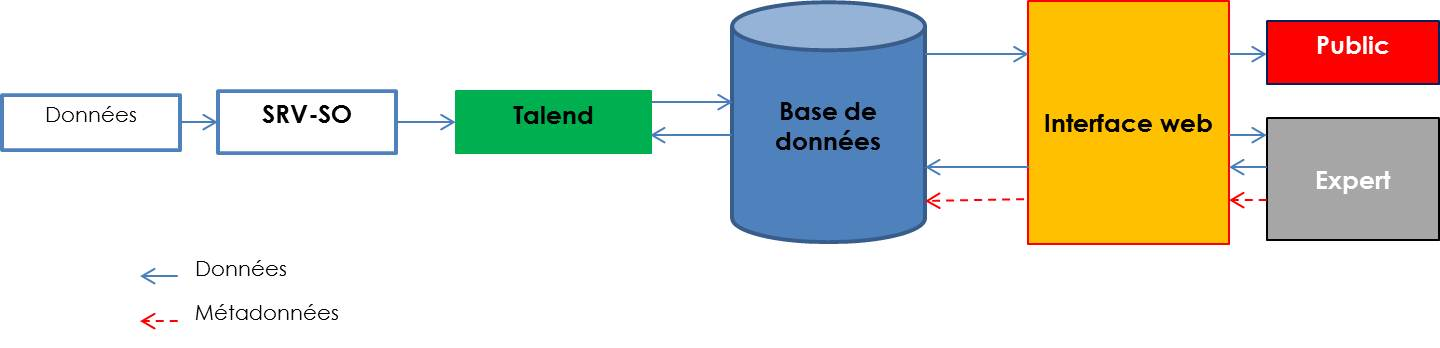
\includegraphics[width=12cm]{sie_0.jpg}
		\caption{Sch�ma global des flux de donn�es et de m�tadonn�es.}
		\label{Fig.1}
	\end{figure}


\subsection{Des capteurs vers le serveur SRV-SO}

\paragraph{Cas 1 : donn�es acquises � haute fr�quences et t�l�-transmises}

\

Les donn�es acquises � haute fr�quence et t�l�-transmises proviennent des 2 (ou 3) stations m�t�o-sol (\#001, \#002, \#003) et de la tour eddy covariance (\#004). Les variables mesur�es sur le sites du SNO Tourbi�res sont les m�mes dans tous les sites. Cependant, suivant les circonstances particuli�res � chaque site, la r�partition de l'ensemble des capteurs, et donc des donn�es qui en r�sultent, peut �tre diff�rente entre les sites. Par cons�quent, le programme des stations peuvent �tre diff�rents (Fig. 2.2). Entre les sites, les fichiers g�n�r�s par les stations ne sont donc pas exactement les m�mes en ce qui concerne l'ordre des variables. Chaque fichier a un nom et des ent�tes de colonnes qui respectent obligatoirement la nomenclature d�crite dans le premier chapitre. De cette mani�re, quelque soit l'ordre des variables, Talend est capable de reconna�tre le site, la station d'acquisition, les variables et les param�tres de celles-ci. Pour chaque site, les fichiers de donn�es en sortie de capteur sont envoy�s dans le dossier "data" correspondant se trouvant sur le serveur SRV-SO localis�s � l'OSUC.

	\begin{figure}[h] 
		\centering
		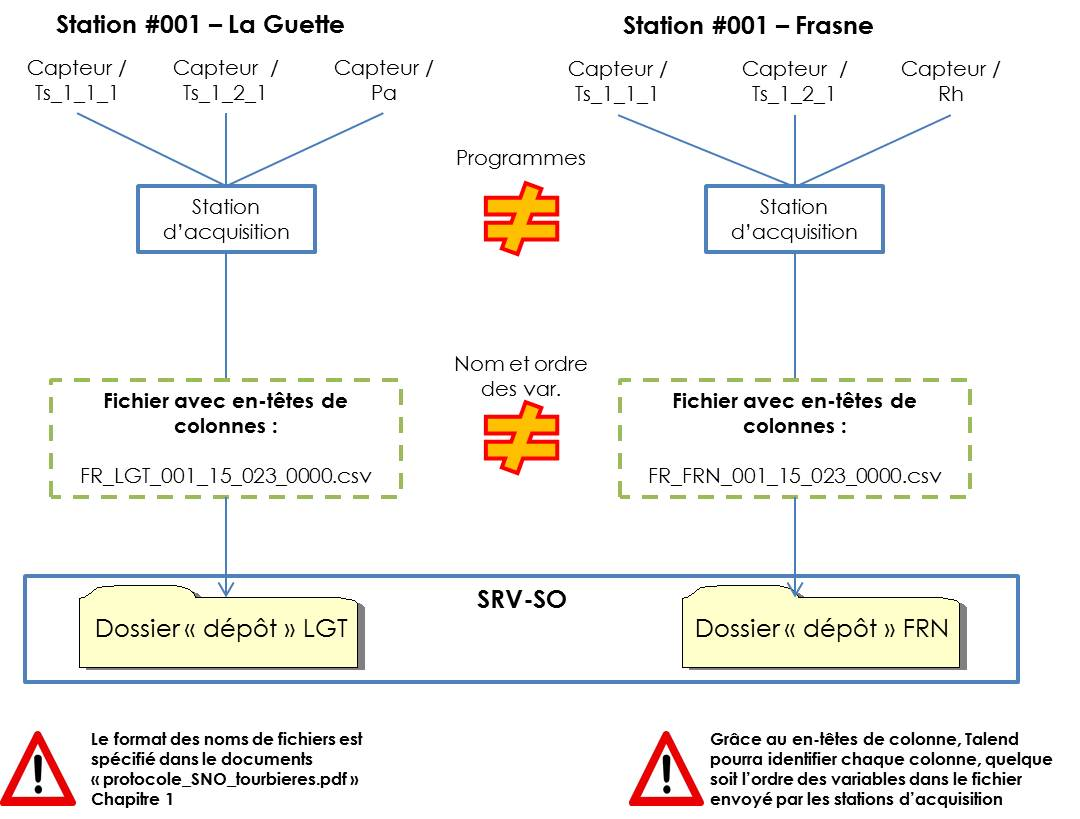
\includegraphics[width=12cm]{sie_1.jpg}
		\caption{Flux de donn�es des \textbf{capteurs} vers \textbf{SRV-SO} des variables acquises  � \textbf{haute fr�quence}, r�guli�rement et \textbf{t�l�-transmises}.}
		\label{Fig.2}
	\end{figure}



\paragraph{Cas 2 : donn�es acquises � haute fr�quences et charg�es par un op�rateur}

\

Les donn�es acquises � haute fr�quence et transmises sur le SRV-SO par un op�rateur proviennent du fluorim�tre � l'�xutoire (station \#005)  et des sondes de niveau de la nappe d'eau (station de \#006 � \#020). Ces stations d'acquisition sont visit�es � intervalles r�guliers par un op�rateur qui, en plus de r�cup�rer les donn�es, assure la maintenance de ces �quipements. Avec un ordinateur de terrain, l'op�rateur se connecte sur la sonde avec un cable adapt� et r�cup�re 1 � plusieurs fichiers. Ces fichiers ne sont pas n�cessairement au format recommand�s (voir chapitre 1). Il est du ressort de l'op�rateur/expert de formater les fichiers sans faire aucun traitement sur les donn�es (donn�es en sortie de capteur) et de les d�poser dans le dossier "data" correspondant sur le seveur SRV-SO, de mani�res � �tre visibles et traitables par Talend .

	\begin{figure}[h] 
		\centering
		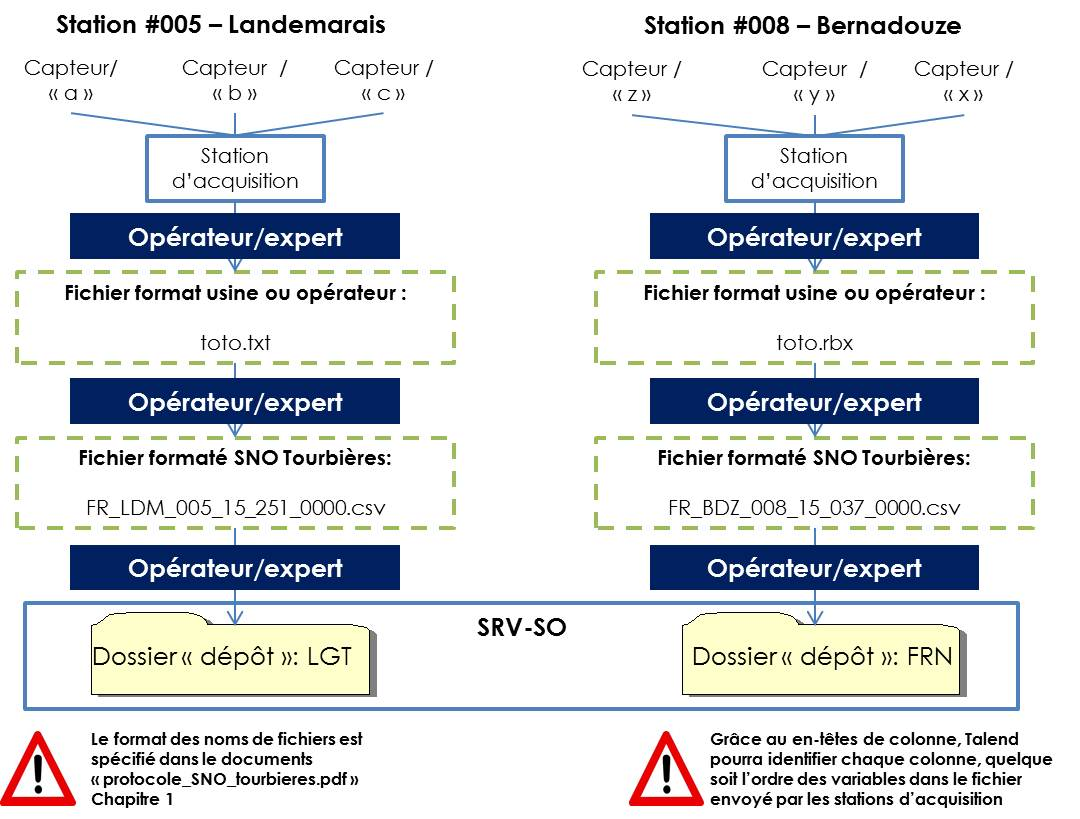
\includegraphics[width=12cm]{sie_2.jpg}
		\caption{Flux de donn�es des \textbf{capteurs} vers \textbf{SRV-SO} des variables acquises  � \textbf{haute fr�quence}, r�guli�rement et \textbf{transmises par un op�rateur}.}
		\label{Fig.3}
	\end{figure}



\paragraph{Cas 3 : donn�es acquises � basse fr�quences et charg�es par un op�rateur}

\

Les donn�es acquises � basse fr�quence et transmises sur le SRV-SO par un op�rateur proviennent des mesures de flux de C par les chambres d'accumulation et des variables associ�es (�quipements de \#101 � \#109), les mesures biog�ochimiques (�quipements de \#110 � \#112) et les mesures manuelles de niveau d'eau (�quipement \#113). L'op�rateur/expert formate les donn�es en suivant les recommandations sp�cifi�es. Les informations concernant le(s) op�rateur(s) et expert(s), les �quipements, les m�thode de mesures, d'analyse et/ou de traitements des donn�es seront pr�cis�es dans les m�tadonn�es. L'op�rateur/expert d�posera les donn�es dans le dossier correspondant sur le serveur SRV-SO (Fig. 2.4)



	\begin{figure}[h] 
		\centering
		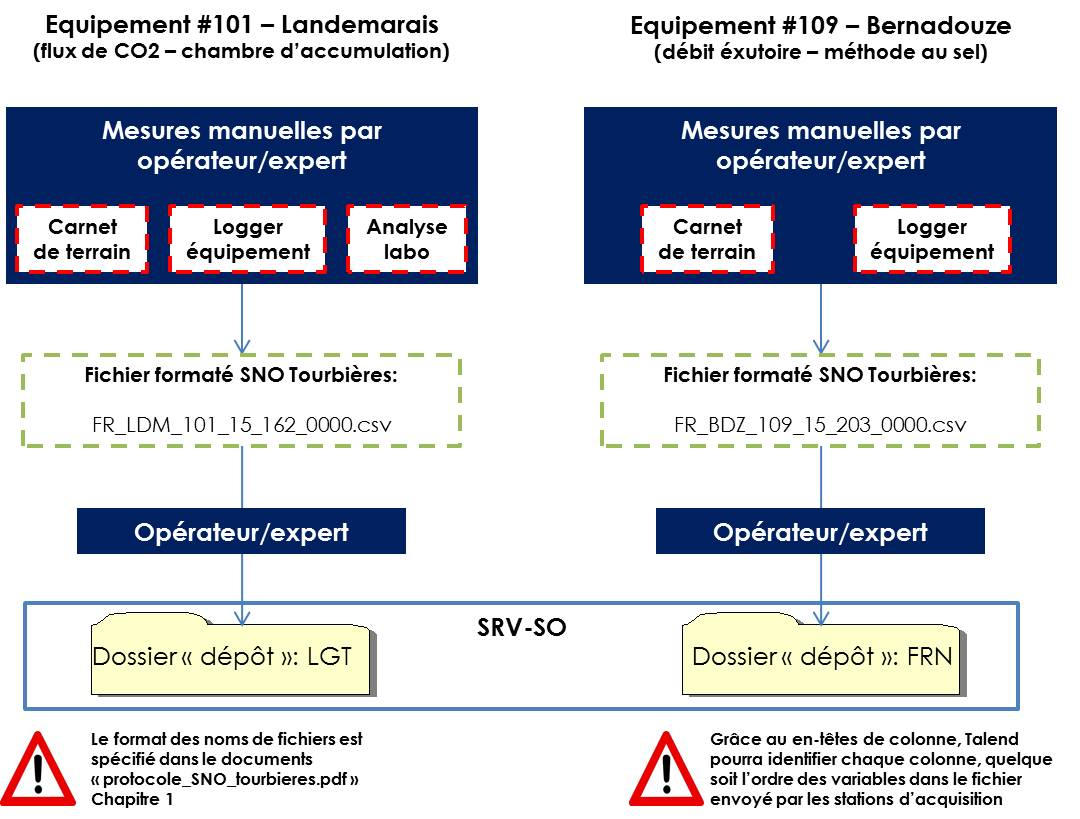
\includegraphics[width=12cm]{sie_3.jpg}
		\caption{Flux de donn�es \textbf{capteur - SRV-SO} des variables acquises  � \textbf{basse fr�quence}, irr�guli�rement (mesures manuelles sur le terrain ou au laboratoire) et \textbf{transmises par un op�rateur}.}
		\label{Fig.4}
	\end{figure}

	

\subsection{L'arborescence du serveur SRV-SO}

Sur le serveur SRV-SO se trouve un dossier "data" qui contient toute les donn�es � inclure dans le SIE. A l'int�rieur de ce dossier se trouve 4 dossiers correspondant aux 4 sites du SNO Tourbi�res. L'acc�s � ces donn�es qui doit �tre r�gul�. Pour chaque site, 3 dossiers sont pr�sents: "data brutes" correspondant aux donn�es avec un �tat d'�laboration le moins d�velopp� (souvent data en sortie de capteur, cf subsection 1.3.1), "data �chec" et "data corrig�es. Le dossiers "data brutes" contient les fichiers de donn�es brutes provenant des stations d'acquisitions et des mesures manuelles (si ces derni�res subissent un traitement, il devra �tre pr�cis� dans les m�tadonn�es). Les donn�es des stations de \#001 � \#004 sont transmises tous les jours et toutes les autres sont transmises annuellement. Le dossiers "data �chec" contient les fichiers de donn�es n'ayant pas pass� les tests r�alis�s par Talend. Le dossiers "data corrig�es" contient les fichiers de donn�es corrig�es apr�s analyses des donn�es flagu�es lors des tests. Les modifications devront �tres consign�es dans les m�tadonn�es.

	\begin{figure}[h] 
		\centering
		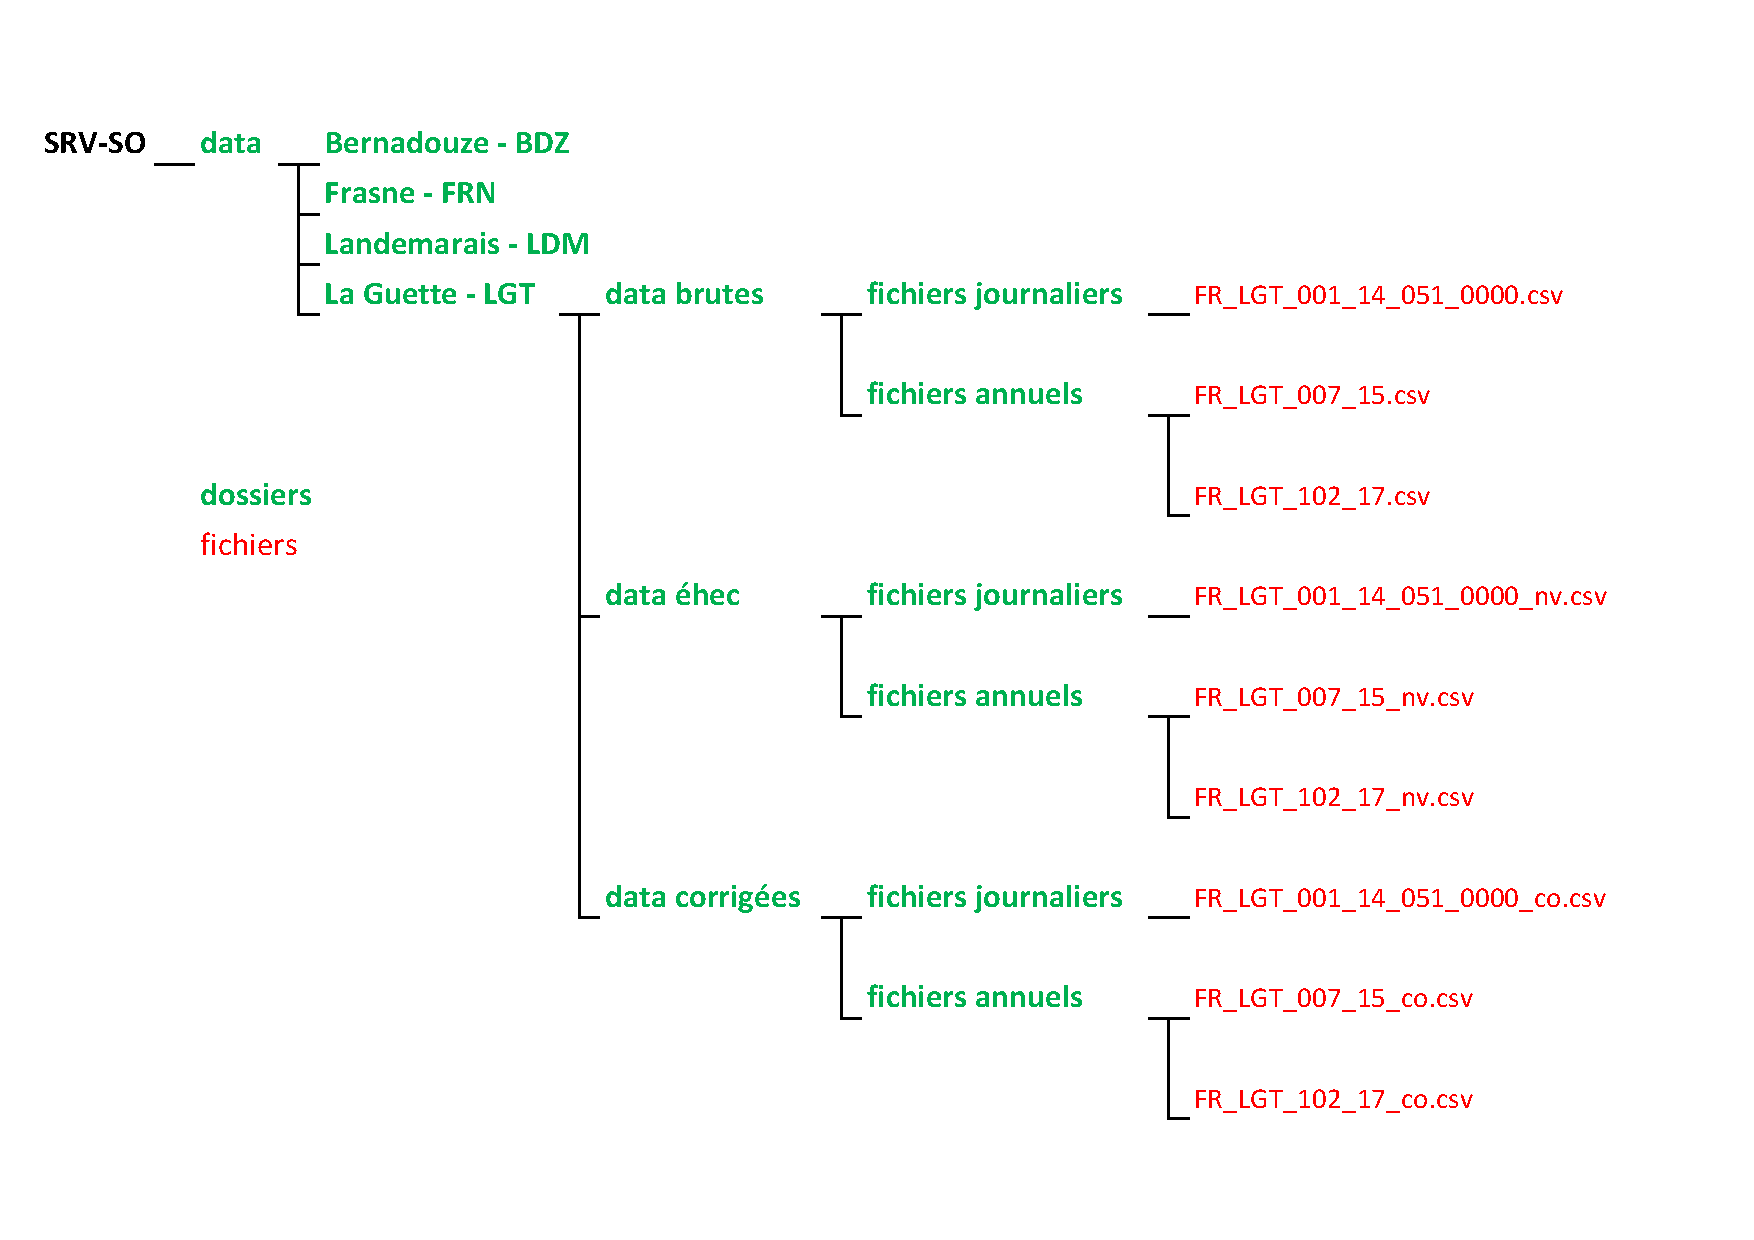
\includegraphics[width=14cm]{arbo_srv_so_1.pdf}
		\caption{Arborescence du SRV-SO. Les types de donn�es et les stations/�quipement concern�s sont pr�cis�s}
		\label{Fig.5}
	\end{figure}


Les fichiers journaliers correspondent aux donn�es acquises � hautes fr�quences et t�l�transmises tous les jours (stations de 001 � 005). Les fichiers annuels correspondent aux donn�es acquises soit � hautes (stations de 005 � 020) ou � basses fr�quences (�quipements de 101 � 110), mais dans les 2 cas transmises par un op�rateur/expert avec une fr�quence minimale d'au moins une fois par an. Pour chaque fichier de donn�es brutes dans lesquels des �checs ont �t� observ�s, un fichier .csv sera g�n�r� avec un "nv" pour "non-valid�" listant les donn�es ne passant pas les tests. Pour chaque fichier de donn�es en �chec (xxx\_nv.csv), un fichier xxx\_ co.csv sera produit par l'expert avec "co" pour "corrig�" listant les donn�es corrig�es.

\subsection{De SRV-SO � la base de donn�es par Talend}

Avant d'�tre int�gr�s dans la base, Talend r�alise des tests sur les donn�es. Il va chercher les donn�es brutes sur SRV-SO (Fig 2.6). Gr�ce au nom des fichiers, il est capable de situ� le jeu de donn�es dans l'espace et le temps. Avec les ent�tes de colonnes, Talend est capable de conna�tre la variables et sa localisation dans le profil. En parall�le, il extrait de la base des donn�es d�j� valid�es. Il calcul � partir de ces donn�es une dispersion autour de la moyenne (e.g. d�viation standard) et un intervalle + ou - 95\%. Il confronte les donn�es non-valid�es � cette intervalle. Talend flague les donn�es tombant dans l'intervalle comme valide avec un "v" et les donn�es hors de l'intervalle comme non-valide "nv". Un fichier avec un "nv" ajout� au nom du fichier brut est g�n�r� regroupant les donn�es non valides et envoy� dans le dossier "�chec" du SRV-SO (Fig 2.6). Les fichiers de donn�es contiendront un "co" pour corrig� dans leur nom et les donn�es corrig�es seront flagu�es avec "v" pour valid�s.

	\begin{figure}[h] 
		\centering
		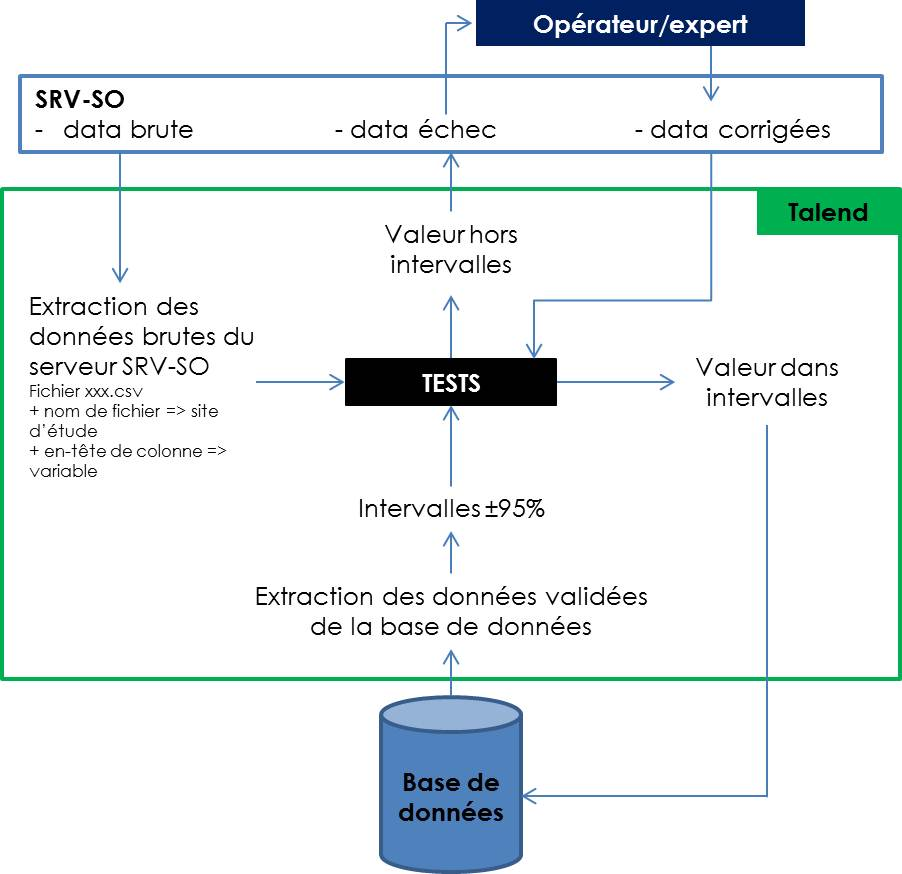
\includegraphics[width=9cm]{sie_4.jpg}
		\caption{Flux de donn�es li�s � l'int�grateur de donn�es Talend (r�alis� � partir du sch�ma propos� par A. Hertout).}
		\label{Fig.6}
	\end{figure}
	



\subsection{De la base de donn�es au public}

Les donn�es brutes, corrig�es et calcul�es pourront �tre visualis�es et t�l�charg�es par tout le monde � partir de l'interface web de la base de donn�es, acc�ssible sur le site web du SNO Tourbi�res: \url{http://www.sno-tourbieres.cnrs.fr/spip.php?article4}.


\subsection{Intervention de l'expert sur les donn�es}

L'intervention sur les donn�es par un expert se produit dans diff�rents cas de figures:

\

	\begin{itemize}
		\item 1. donn�es flagu�es non-valide par Taland n�cessitant une correction
		
		\
		
		\item 2. donn�es flagu�es non-valide par Talend ne n�cessitant pas de correction
		
		\
		
		\item 3. donn�es flagu�es valide par talend n�cessitant une correction
		
		\
		
		\item 4. donn�es n�cessitant un ajustement � cause d'une d�rive
		
		\
		
		\item 5. calcul de nouvelles variables � partir des donn�es corrig�es
	\end{itemize}
	
\
\paragraph{Cas 1.}	
Une fois le traitement Talend effectu�, l'expert analyse les donn�es qui ont �t� r�pertori�es dans le fichier �chec. Les donn�es flagu�es non-valide sont effectivement incorrectes. L'expert r�alise les corrections et d�posent les donn�es dans le fichier "data corrig�es" et les donn�es sont trait�es de nouveau par Talend. Les fichiers log correspondant (cf section flux des m�tadonn�es) devront �tre renseign�s.

\paragraph{Cas 2.}	
Une fois le traitement Talend effectu�, l'expert analyse les donn�es qui ont �t� r�pertori�es dans le fichier �chec. Les donn�es flagu�es non-valide sont en fait correctes. Elles correspondent soit aux extr�mas de la loi normale, soit � des �v�nements particuliers qui sorte de la loi normale. L'expert ne r�alise pas de corrections et il doit �tre en mesure de changer le flag de donn�es particuli�res via l'interface web. Les fichiers log correspondant (cf section flux des m�tadonn�es) devront �tre renseign�s.

\paragraph{Cas 3.}	
Une fois le traitement Talend effectu�, l'expert visualise sur l'interface web les donn�es qui ont �t� flagu�es comme valides. Des donn�es flagu�es valide peuvent se r�v�ler �tre incorrecte. Elles peuvent correspondre � des donn�es entrant dans l'intervalle, mais irr�aliste (exemple: temp�rature de l'air � -1�C au mois de juillet pendant une mesure). L'expert r�alise les corrections et d�posent les donn�es dans le fichier "data corrig�es" et les donn�es sont trait�es de nouveau par Talend. Les fichiers log correspondant (cf section flux des m�tadonn�es) devront �tre renseign�s.

\paragraph{Cas 4.}
Certain capteur peuvent d�river. Quand un suivi de la d�rive est r�alis� (e.g. capteur de pluviom�trie) ou quand un capteur similaire de secours est disponible (e.g. capteur de luminosit� � la tourbi�re des Landes � 10 km de La Guette), un calcul de d�rive est possible. Ces calculs n'�tant par d�finition pas pr�visible, il est difficile d'automatiser ces proc�dures. L'expert r�alise donc lui m�me la proc�dure de d�rive et d�pose les donn�es corrig�es dans le dossier "data corrig�es".  Les fichiers log correspondant (cf section flux des m�tadonn�es) devront �tre renseign�s.

\paragraph{Cas 5.}
L'expert peut calculer des nouvelles variables d'int�r�t � partir des variable d�j� enregistr�es sur le base de donn�es, comme par exemple l'�vapotranspiration potentielle. Si possible, ces calculs seront automatis�s par l'int�grateur de donn�es Talend. Si ce n'est pas possible, l'expert devra �tre capable de rentrer les donn�es calcul�es � partir de la base de donn�es. Les fichiers log correspondant (cf section flux des m�tadonn�es) devront �tre renseign�s.

\newpage

\section{Flux des m�tadonn�es}

\subsection{Sur les capteurs}
Une fiche de m�tadonn�es doit �tre remplie pour chaque capteur install� ayant ou en train de g�n�rer des donn�es. Les renseignements devront �tre les suivant:

	\begin{itemize}
		\item mod�le (avec num�ro de s�rie si possible)

		\item variable(s) mesur�e(s)

		\item pr�cision, justesse de la (des) mesure(s)

		\item site(s) d'installation et point GPS	
		
		\item date de la premi�re mesure
		
		\item date de la derni�re mesure si capteur HS		
		
		\item installateur(s)
				
		\item personne(s) en charge de la maintenance
		
		\item expert(s) de la (des) variable(s) g�n�r�e(s) par le capteur
		
		\item historiques des �v�nement intervenu sur ce capteur
	\end{itemize}
	

\subsection{Sur les variables g�n�r�es par les capteurs ou les �quipements}
Une fiche de m�tadonn�es doit �tre remplie pour chaque variable ayant �t� mesur�e ou en cours de mesure sur le terrain ou au laboratoire. Les renseignements devront �tre les suivant:


	\begin{itemize}
		\item nom de la variable

		\item code

		\item mod�le du capteur (avec num�ro de s�rie si possible) pour chaque p�riode de mesure
		
		\item p�riode d'acquisition pour chaque capteur si plusieurs capteurs ont �t� utilis�
		
		\item calcul de la variable r�alis�e par la sonde si r�alis�
		
		\item post-traitement 1 : test Talend et r�sultats
		
		\item post-traitement 2 : calcul de calibration, toutes informations sur la calibration

		\item expert(s) en charge de valider la variable
	\end{itemize}
	
\subsection{Sur les variables cacul�es}
Une fiche de m�tadonn�es doit �tre remplie pour chaque variable calcul�e � partir des donn�es g�n�r�es par les capteurs (e.g. �). Les renseignements devront �tre les suivant:


	\begin{itemize}
		\item nom de la variable

		\item code

		\item nom des variables utilis�es pour les calculs
		
		\item d�tails des calculs
		
		\item post-traitement 1 : test Talend et r�sultats
		
		\item post-traitement 2 : calcul de calibration, toutes informations sur la calibration

		\item expert(s) en charge de valid� la variable
	\end{itemize}
	

\newpage

\section{Gestion de l'acc�s au serveur SRV-SO}

L'acc�s au serveur SRV-SO sera pour tout ou partie accord� � un nombre restreint de membres du SNO Tourbi�res. Les personnes ayant acc�s � tout le serveur sont:

	\begin{itemize}
		
		\item \textbf{Laurent Catherine} - informaticien OSUC
		
		
		\item \textbf{Yohan Brossard} - informaticien OSUC
		
		
		
		\item \textbf{Laurent Perdereau} - acquisition et transmission des donn�es
		
		
		
		\item \textbf{St�phane Binet} - hydrologie des sites du SNO Tourbi�res
		
		
		
		\item \textbf{Fatima Laggoun} - coordinatrice du SNO Tourbi�res et responsable du site "La Guette"
		
		
		
		\item \textbf{S�bastien Gogo} - coordinateur du SNO Tourbi�res et responsable du site "La Guette"
	\end{itemize}
	
\
	
Les personnes ayant acc�s aux dossiers du site de Bernadouze sont:

	\begin{itemize}
		\item \textbf{Didier Galop}
		
		
		
		\item \textbf{Laure Gandois}
				
				
				
		\item \textbf{Emilie Lerigoleur}
				
				
				
		\item \textbf{Ga�l Leroux}
	\end{itemize}
	
\
	
Les personnes ayant acc�s aux dossiers du site de Frasne sont:

	\begin{itemize}
		\item \textbf{Daniel Gilbert}
		
		
		
		\item \textbf{Marie-Laure Toussaint}
		
		
		
		\item \textbf{Catherine Bertrand}	
	\end{itemize}
	
\
	
Les personnes ayant acc�s aux dossiers du site de Landemarais sont:

	\begin{itemize}
		\item \textbf{Andr�-Jean Francez}
		
		
		
		\item \textbf{Guillaume Bouger}
		
		
		\item \textbf{Laurent Jeanneau}
	\end{itemize}
	
\

D'autres personnes pourront avoir acc�s au fichiers sur demande aupr�s des informaticiens de l'OSUC et validation par les coordinateurs. 
	
\newpage

%\section{Gestion de l'interaction avec la base de donn�e par l'interface web}

%\newpage

\section{Gestion des t�l�chargement des donn�es}

Les donn�es doivent �tre le plus librement accessibles au public, scientifique ou non. Elles pourront �tre t�l�chargeable � partir de l'interface web de la base de donn�es. Les informations suivantes devront �tre renseign�es dans un formulaire:

	\begin{itemize}
		\item site
		\item date de d�but
		\item date de fin
		\item variables(s)
		\item donn�es pas encore valid�es avec log des variables et capteurs correspondant
		\item donn�es valid�es avec log log des variables, des capteurs et des corrections correspondant
	\end{itemize}
	
Apr�s la premi�re ligne du fichier t�l�charg� contenant les codes des variables, seront indiqu�s dans une deuxi�me ligne les unit�s.
	
Une fois que l'internaute aura rempli le formulaire et valid� sa demande, une fen�tre d'information lui indiquera qu'il pourra librement utiliser les donn�es � condition d'inclure le SNO Tourbi�res dans les remerciements des articles scientifiques dont les donn�es t�l�charg�es seront le support et si possible de pr�venir les coordinateurs du SNO Tourbi�res de la publication de ces articles. Une fois coch�e la case : "j'ai pris connaissance de la condition requise pour utiliser les donn�es", les donn�es seront directement mise � disposition au format .csv (fen�tre d'enregistrement classique) sans le besoin d'une validation de la demande par un responsable du SNO Tourbi�res. Aucun courriel, ni nom, ni organismes seront demand�s et par cons�quent enregistr�s. Aucune demande � la CNIL ne sera n�cessaire. Les informations enregistr�es seront juste les suivantes: nombre des visites de l'interface web, nombre de fichiers de donn�es t�l�charg� avec les variables demand�es.




\newpage

		%--- CHAPITRE 3 : Variables m�t�o-sol
		
%-------------------------------- %   Chapitre 3   %--------------------------------- %


% % % % % % % % % % % % % % % % % % % % % % % % % % % % % % % % % % % % % % % % % % % %
%																					  %	
%   		SNO Tourbi�res - Variables m�t�orologique et physique du sol		      %
%																					  %	
% % % % % % % % % % % % % % % % % % % % % % % % % % % % % % % % % % % % % % % % % % % %





\chapter{Variables m�t�orologique et physique du sol}\label{v_meteosol}

S. Gogo, ...

\section{Cadre et objectif des mesures}
Le pr�sent document porte sur toutes les mesures acquises par les stations d'acquisition, g�n�ralement des CR1000 (Campbell), pr�sentes sur chaque site du service national d'observation (SNO) Tourbi�res et d�di�es aux mesures m�t�orologique et de la physique du sol. La majorit� des informations proviennent des manuels d'utilisation fournis par le fabriquant ou le revendeur.

Les indications de positionnement des capteurs doivent �tre suivies au mieux. Tout �cart aux positionnement standard doivent �tre sp�cifi�s pour �valuer la qualit� des donn�es.

\textbf{L'objectif de ces mesures sont:}

\

		\begin{itemize}
			\item \textbf{caract�riser d'un point de vue climatique chaque site}
			
			\
			
			\item \textbf{compl�ter les mesures pour l'�tude du bilan hydrologique de chaque site (pluviom�trie, �vapotranspiration)}
			
			\
			
			\item \textbf{fournir des donn�es pour r�aliser le "gap filling" des donn�es acquises par le syst�me d'Eddy Covariance}
			
			\
			
			\item \textbf{permettre le contr�le et l'assurance de la qualit� des donn�es acquises par le syst�me d'Eddy Covariance}
			
			\
			
			\item \textbf{aider � l'interpr�tation des donn�es acquises par le syst�me d'Eddy Covariance}
			
			\
			
			\item \textbf{fournir des donn�es pour la mod�lisation dans le cadre du SNO Tourbi�res ou de tout autre programme de recherche (mise � disposition des donn�es)}
		\end{itemize}

\newpage

\section{Organisation des �quipements}


\subsection{Nombre de station d'acquisition}
Sur chaque site du r�seau, il y aura un minimum de 2 stations d'acquisition pour les variables m�t�orologique et physique du sol: la station \#001 pour les mesures m�t�orologiques et un premier profil de sol et la station \#002 pour les mesures du deuxi�me profile de sol. Une troisi�me station est th�oriquement pr�vue (\#003). Nous adopterons le nombre et la nomenclature des variables recommand�es par ICOS pour les sites de niveau 2.

\subsection{Installation des stations}
Les capteurs m�t�orologiques devront �tre install�s en hauteur (environ 2m) et de mani�re � �viter le plus possible des perturbations (v�g�tation de taille haute le plus loin possible). L'installation sur une plateforme est recommand�e.

Pour �tre repr�sentatifs des conditions dans l'empreinte des mesures de flux par eddy covariance, les capteurs de physique du sol devront �tre install�s sous la v�g�tation dominante dans l'empreinte. Si l'empreinte est couverte � part �gale de 2 types de v�g�tations, une station sera mise dans chaque type de v�g�tation.

Pour des raisons pratiques, les capteurs de physique du sol du profil 1 seront branch�es sur la station m�t�orologiques (station m�t�o-sol \#001, m�t�o classique + sol). Egalement pour des raisons partiques, les capteurs du deuxi�me profil pourront �tre branch�s sur une deuxi�me station d'acquisition (\#002)  install�es sur le tr�pied supportant les capteurs de mesure de flux par eddy covariance.

\newpage

\section{Les variables: mesures, nomenclature, et capteurs}

	
Les d�tails des informations concernant les noms de fichier, le nombre et le type de variables et leur code sont disponibles dans le chapitre 1.

Pour rappel voici la liste des variables cibles concern�es par ce chapitre.


	\textbf{code variable:}
		\begin{itemize}	
			\item 	\textbf{Pa} = pression atmosph�rique
			\item 	\textbf{P\_rain} = pr�cipitation sous forme de pluie
			\item 	\textbf{PPFD} = photosynthetic photon flux density
			\item 	\textbf{WS} = vitesse du vent
			\item 	\textbf{WD} = direction du vent
			\item 	\textbf{RH} = humidit� relative de l'air
			\item 	\textbf{Ta} = temp�rature de l'air
			\item 	\textbf{Ts} = temp�rature du sol
			\item 	\textbf{SWC} = teneur en eau du sol
			\item 	\textbf{G} = flux de chaleur dans le sol
			\item 	\textbf{GWL} = niveau de la nappe d'eau	
			\item 	\textbf{SWin} = ondes courtes entrantes
			\item 	\textbf{SWout} = ondes courtes sortantes
			\item 	\textbf{LWin} = ondes longues entrantes
			\item 	\textbf{LWout} = ondes longues sortantes
		\end{itemize}

\

Plusieurs variables peuvent �tre acquises par un m�me instrument, exemple: la vitesse et la direction du vent sont mesur� par un an�mom�tre (e.g. Wind Sonic de Gill).




\subsection{Les capteurs}
M�me si compte-tenu des contraintes de tous ordres, l'uniformisation du parc analytique sera difficile, les membres du SNO Tourbi�res s'engage � tendre vers cette uniformisation  pour une meilleure comparaison entre site et pour diminuer la complexit� de la gestion des �quipements et des donn�es (un �quipement diff�rent dans chaque site pour une m�me variables implique 4 fournisseur diff�rents, etc...).

\

Les �quipements dont on se propose l'installation sur les sites respectent au mieux les recommandations ICOS (tableau 3.1).


\begin{table}
%\begin{scriptsize}

\caption{Liste des capteurs correspondant au variables cibles obligatoires et leur nombres dans une configuration minimale.}
\label{Table 2.}

		\begin{tabular}{lll1}
			\hline
			\textbf{Variable}&\textbf{Mod�le}&\textbf{Marque}&\textbf{N}\\
			\hline
			Pression atmosph�rique&PTU300&Vaisala&1 \\
			Pluviom�trie&ARG100&Campbell&1  \\
			Rayonnement photosynth�tique actif&SKP215&Campbell&1 \\
			Vitesse du vent&Windsonic&Gill&1 \\
			Direction du vent&Windsonic&Gill&1 \\
			Humidit� relative de l'air&HMP155A&Vaisala&1 \\
			Temp�rature de l'air&HMP155A&Vaisala&1 \\
			Temp�rature du sol&107&Campbell&16 \\
			Teneur en eau du sol&CS650&Campbell&8  \\
			Flux de chaleur dans le sol&HFP01SC&Hukseflux&4 \\
			Niveau de la nappe d'eau&CS451&Campbell&2 \\
			Ondes courtes entrantes&CNR4&Kipp-Zonen&1 \\
			Ondes courtes sortantes&CNR4&Kipp-Zonen&1 \\
			Ondes longues entrantes&CNR4&Kipp-Zonen&1 \\
			Ondes longues sortantes&CNR4&Kipp-Zonen&1 \\			
			\hline
		\end{tabular}
%\end{scriptsize}
\end{table}


%Tableau 2. Consommation �lectrique de chaque capteur et de la station d'acquisition dans les conditions de mesures �tablies (une mesure toutes les 15 secondes, moyenne sur 30 minutes).

La suite du document d�taille les principe de mesure de chaque capteurs, donne des pr�cision �ventuelles sur son positionnement et sa maintenance, ainsi que tous les calculs n�cessaire � l'�laboration de la variable cible (signaux du capteurs, d�rive, calibration)

\newpage


\section{Pression atmosph�rique - Pa - PTU300}

\subsection{Principe de mesure et unit�}

\subsection{Positionnement du capteur}

\subsection{Maintenance du capteur}

\subsection{Elaboration de la variable cible}

\paragraph{Calibration et d�rive du capteur}

\paragraph{Calcul de la variable cible et autres variables}


\newpage

\section{Pluviom�trie - P\_rain - ARG100}

\subsection{Principe de mesure et unit�}
L'ARG100 est un pluviom�tre � augets basculeurs. Il est constitu� d'un entonnoir qui r�cup�re la pluie et d'une base. La base est constitu� de deux partie. La partie int�rieure contient les augets (Fig.\ref{Fig.1}). La partie externe est fix� sur une plaque en fer install�e sur un support stable. 

La pluie qui entre dans l'entonnoir est dirig�e vers un des deux augets. Quand celui-ci est rempli d'une quantit� d�termin�e correspondant � 0.2 mm de pr�cipitation, il bascule permettant sa vidange et le mise en position du deuxi�me auget qui se rempli � son tour. Un bras est fix� aux augets (Fig.\ref{Fig.1}) et � chaque bascule, le mouvement du bras force un aimant � passer devant un commutateur � lame souple (Fig.\ref{Fig.1}), cr�ant un contact pendant quelques milisecondes. Le nombre de bascule est ainsi compt� et enregistr� par la centrale
d'acquisition.

L'unit� de mesure est le millim�tre, mm.
	\begin{figure}[h] 
		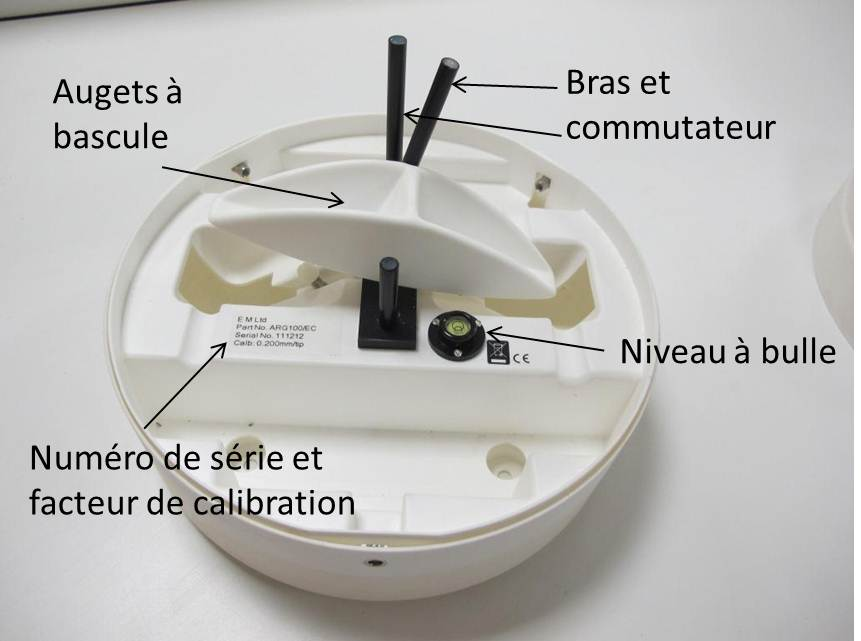
\includegraphics[width=14cm]{arg100complegende.jpg}
		\caption{Partie int�rieure de l'ARG100.}
		\label{Fig.1}
	\end{figure}

\subsection{Positionnement du capteur}
Le pluviom�tre ARG100 doit �tre plac� horizontalement gr�ce � un niveau � bulle plac� dans le pluviom�tre(Fig.\ref{Fig.1}). Un pluviom�tre affecte la circulation de l'air (flux et turbulence augment�es). Cependant, l'ARG100 a un profil qui permet de limiter ces biais. Aucun obstacle autour du capteur ne doit �tre pr�sent pour intercepter les pr�cipitations. En r�gle g�n�rale, on estime que la distance entre un obstacle et le pluviom�tre doit �tre au moins �gale � deux fois la hauteur de l'obstacle.
Afin d'obtenir des mesures comparables, les ARG100 du SNO Tourbi�res sont plac�s � une hauteur entre 1 et 2 m.


\subsection{Maintenance du capteur}
La maintenance sera effectu�e tous les mois si possible ou au moins tous les 6 mois. Elle consistera en:
	\begin{itemize}
		\item v�rifier que rien n'emp�che la circulation de l'eau,
		\item v�rifier l'int�grit� des c�bles,
		\item v�rifier l'horizontalit� du capteur gr�ce au niveau � bulle,
		\item v�rifier que la balance fonctionne bien en versant un volume connu d'eau et en comptant le nombre de bascule (� faire en m�me temps que la mesure de la d�rive),
		\item si besoin, ramener le capteur au laboratoire pour un nettoyage complet de l'ext�rieur et de l'int�rieur (prolif�ration de micro-algues)
	\end{itemize}

\subsection{Calibration et d�rive du capteur}
L'ARG100 est calibr� par le fabricant. Un facteur de calibration est donn� sur un certificat et �galement inscrit dans la partie int�rieur du pluviom�tre (Fig.\ref{Fig.1}).

La d�rive du capteur est test�e le plus fr�quemment possible en m�me temps que l'inspection de la balance. Il s'agit de verser � une date connue une quantit� connue d'eau dans le pluviom�tre. La comparaison entre les millim�tres d'eau apport�s et les millim�tres d'eau estim�s par le pluviom�tre permettra d'estimer une possible d�rive de la mesure de l'appareil dans le temps.

Si la d�rive augmente avec le temps, une calibration en deux temps devra �tre r�alis�e: 
	\begin{enumerate}
		\item Ajustement et calibration statique: il s'agit de r�gler la bascule pour la quantit� d'eau �quivalente � 0.2 mm � l'aide des vices de calibration,
		\item Calibration dynamique: il s'agit de faire passer dans le pluviom�tre 810.4 cm$^3$ d'eau contenu dans un r�servoir (� un d�nit correspondant � 100 min pour vider le r�servoir). A la fin, 80 bascules doit th�oriquement se produire et le nombre exacte et obtenu par le datalogger en ajoutant la fraction restante dans un des deux augets. Si N est le nombre de bascule + fraction restante, le facteur de calibration sera: FC = 0.2 x 80/N. 
	\end{enumerate}

\newpage

%\section{Hauteur de neige - P\_snow - SR50A}

%\subsection{Principe de mesure et unit�}

%\subsection{Positionnement du capteur}

%\subsection{Maintenance du capteur}

%\subsection{Calibration et d�rive du capteur}

%\newpage

\section{Les mesures de rayonnement - SWin, SWout, LWin, LWout - CNR4 }

\subsection{Principe de mesure et unit�}
La mesure du rayonnement est bas� sur le mesure simultan�e de 4 capteurs : 2 pour le rayonnement solaire (ondes courtes ou short wave - SW) appel�s pyranom�tres (Fig. 4), 2 pour le rayonnement infrarouge lointain (ondes longues ou long wave - LW) pyrg�om�tres (Fig. 4). 

%		\begin{figure}[h] 
		%	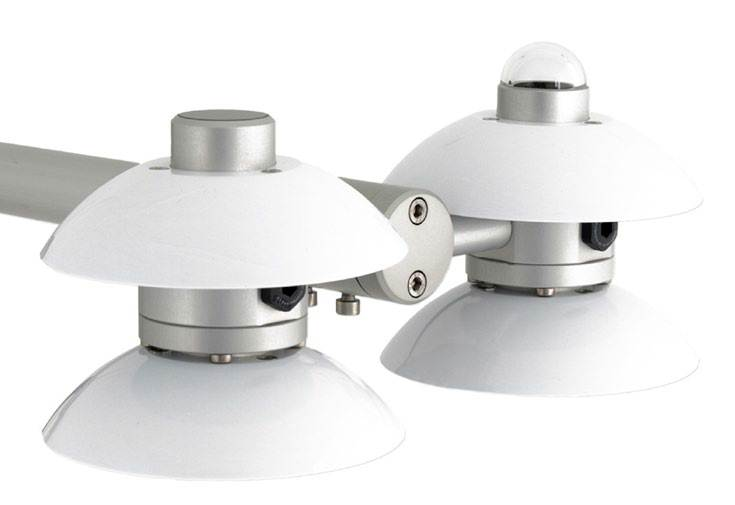
\includegraphics[width=10cm]{NetRad_1.jpg}
			%\caption{Les 2 capteurs sur la gauche correspondent aux pyrgeom�tres et les 2 sur la droite au pyranom�tres. Les 2 capteurs orient�s vers le haut enregistrent les rayonnement entrant et les 2 orient�s vers le bas (cach� par un bouclier de protection) mesurent le rayonnement sortant.}
			%\label{Fig.4}
		%\end{figure}

Pour chaque type d'onde, un capteur est positionn� vers le haut et le deuxi�me vers le bas. La s�paration de tous les capteurs permet d'obtenir un large spectre de variable: 

	\begin{itemize}
		\item rayonnement solaire global ou ondes courtes entrantes: SW$_{in}$
		\item rayonnement solaire r�fl�chi ou ondes courtes sortantes: SW$_{out}$
		\item rayonnement infrarouge �mis par le ciel ou ondes longues entrantes: LW$_{in}$
		\item rayonnement infrarouge �mis par le sol ou ondes longues sortantes: LW$_{out}$
		\item SW "albedo"
		\item "sky temperature"
		\item "ground surface temperature"
		\item rayonnement net: NetRad 
	\end{itemize}
	

Pour calculer les rayonnement, il faut diviser les signaux transmis en volt: "U", par une constante "E" repr�sentant la sensibilit� du capteur. Le rayonnement net est ensuite calcul� � partir des 4 composants mesur�s (SW$_{in}$, SW$_{out}$, LW$_{in}$, LW$_{out}$) de la fa�on suivante\footnote[1]{La temp�rature T$_{pyrgeo}$ pour les formules suivantes doivent �tre en Kelvin. Si les temp�ratures mesur�es sont en Celsius, ajouter 273.15}:

\begin{align}
$  SW$_{in}$ $&=$ U$_{pyrano, up}$/E$_{pyrano, up}$  $\\
$  SW$_{out}$ $&=$ U$_{pyrano, down}$/E$_{pyrano, down}$  $\\
$  LW$_{in}$ $&=$ (U$_{pyrgeo, up}$/E$_{pyrgeo, up}$) + 5.67 $10^{-8}$(T$_{pyrgeo}$)$^{4}$  $\\
$  LW$_{out}$ $&=$ (U$_{pyrgeo, down}$/E$_{pyrgeo, down}$) + 5.67 $10^{-8}$(T$_{pyrgeo}$)  $\\
$  SW$_{net}$ $&=$ U$_{pyrano, up}$/E$_{pyrano, up}$ - U$_{pyrano, down}$/E$_{pyrano, down}$  $\\
$  LW$_{net}$ $&=$ U$_{pyrgeo, up}$/E$_{pyrgeo, up}$ - U$_{pyrgeo, down}$/E$_{pyrgeo, down}$  $\\
$  NetRad $&=$ SW$_{net}$ + LW$_{net}$  $
\end{align}

En plus du rayonnement net, d'autre variables peuvent �tre calcul�es

\begin{align}
$  SW$_{albedo}$ $&=$ SW$_{out}$/SW$_{in}$  $\\
$  T$_{surface}$ $&=$ (LW$_{out}$/5.67 $10^{-8}$)$^{1/4}$  $\\
$  T$_{sky}$ $&=$ (LW$_{in}$/5.67 $10^{-8}$)$^{1/4}$  $
\end{align}

\subsection{Positionnement du capteur}

\subsection{Maintenance du capteur}

\subsection{Calibration et d�rive du capteur}
La qualit� des donn�es peut �tre suivie en analysant les tendances du signal absolu du SWin, de l'albedo, de la corr�lation entre SW$_{in}$ et LW$_{in}$, SW pendant la nuit, et la corr�lation entre LW$_{out}$ et la temp�rature de surface. 


\subsection{Informations compl�mentaires}
Les capteurs de rayonnement sont passifs et n'ont donc pas besoin d'�tre branch�s � une batterie. Cependant, le pyrg�om�tre peut �tre chauff� pour �viter la formation de bu�e.

\newpage

\section{Densit� du flux de photons photosynth�tiques - PPFD - SKP215}

\subsection{Principe de mesure et unit�}

\subsection{Positionnement du capteur}

\subsection{Maintenance du capteur}

\subsection{Calibration et d�rive du capteur}

\newpage

%\section{Normalized Difference Vegetation Index - NDVI - Orsay}

%\subsection{Principe de mesure et unit�}

%\subsection{Positionnement du capteur}

%\subsection{Maintenance du capteur}

%\subsection{Calibration et d�rive du capteur}

%\newpage

\section{Vitesse du vent - WS - WindSonic}

\subsection{Principe de mesure et unit�}
Le capteur WindSonic (Gill) 2D mesure le temps mis par un pulse d'ultrason pour parcourir la distance entre le transducteur nord (N) et le transducteur sud (S) et il le compare avec le temps mis par un pulse d'ultrason pour parcourir la distance entre le transducteur sud (S) et le transducteur nord (N, Fig. 5). De m�me, les temps entre les transducteurs ouest (W) et l'est (E), et est et ouest sont compar�s. La vitesse du vent peut alors �tre calcul�e � partir des diff�rences de temps de vol sur chaque axe (Figure 6). Ce calcul est ind�pendant de la temp�rature.

	\begin{figure}[h] 
		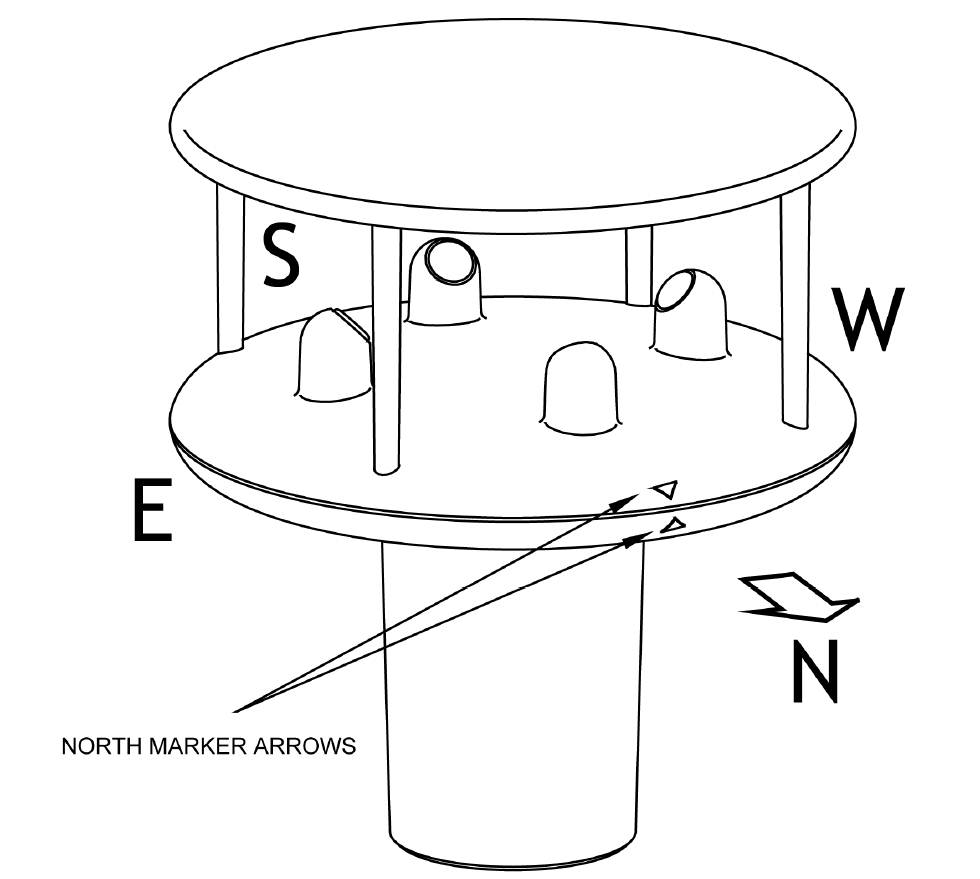
\includegraphics[width=10cm]{WindSonic.jpg}
		\caption{Positions des transducteurs sur le WindSonic.}
		\label{Fig.5}
	\end{figure}


L'unit� de mesure est le m�tre par seconde, m.s$^{-1}$.

L'�tendue de mesure va de 0 � 60 m.s$^1$, avec une pr�cision de l'ordre de 2\% (� 12 m.s$^{-1}$). La r�solution de la mesure est de 0.01 m.s$^{-1}$.
	

\subsection{Positionnement du capteur}
Avant l'installation sur le terrain, le bon fonctionnement du capteur devra �tre v�rifi� au laboratoire : cablage �lectrique, unit�, acquisition. Sur le terrain, le capteur doit �tre plac� sur un tube vertical de mani�re � r�aliser une mesure horizontale.

	\begin{figure}[h] 
		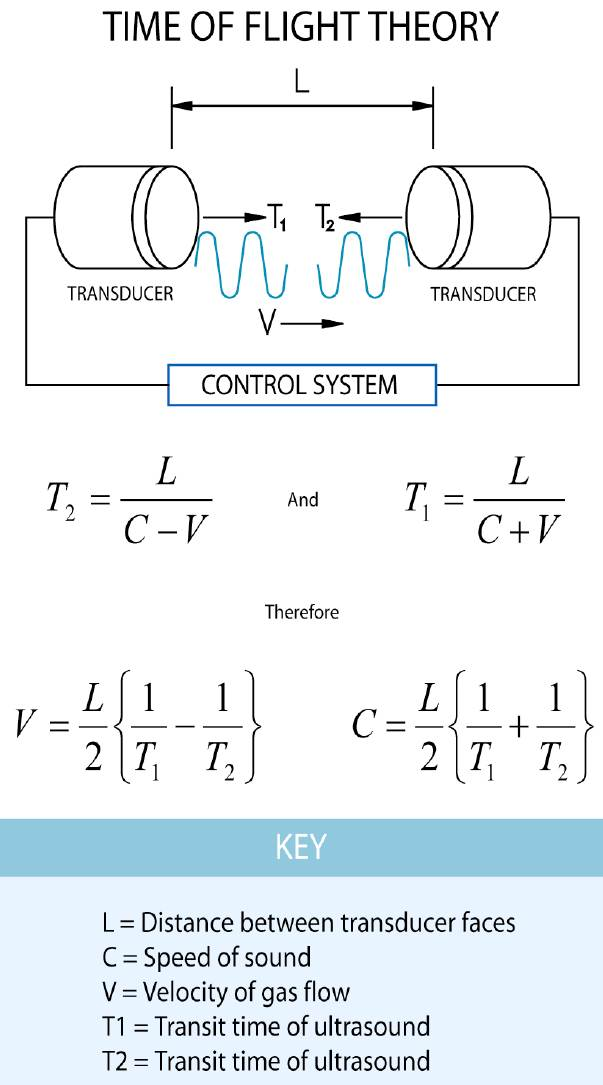
\includegraphics[width=7cm]{WindSonic2.jpg}
		\caption{Calcul de la vitesse du vent avec l'an�mom�tre � ultrasons.}
		\label{Fig.6}
	\end{figure}

Une attention particuli�re sera donn�e � la bonne orientation du capteur. Une fl�che grav�e sur le capteur indiquant le nord doit �tre plac� en direction du \textbf {nord g�ographique}. Le nord magn�tique ne correspond pas au nord  g�ographique. Le jour de l'installation du capteur, ll faut d�terminer la d�clinaison magn�tique terrestre, soit l'angle en un point donn� du globe entre le p�le nord magn�tique et g�ographique. Cet angle peut �tre obtenu, pour la date d'installation du capteur, sur le site suivant: http://www.ngdc.\\noaa.gov/geomag-web/\#declination.

La vitesse du vent intervient dans l'�quation de Penman-Monteith pour calcul de l'�vapotranspiration. Cette �quation a pour pr�suppos� que toutes les mesures des variables intervenant dans l'�quation sont r�alis�es � 2 m au dessus de la surface du sol. Si possible, le capteur sera donc dispos� � une hauteur de 2 m au dessus de la surface de chaque tourbi�re. Dans tous les cas, la hauteur � laquelle se trouve le capteur devra �tre mentionn�e dans les m�tadonn�es de cette variable.

Il devra �tre v�rifi� que le transmission GPRS  et qu'aucun obstacle physique (autres partie de la station m�t�o, arbres � proximit�) n'affecte la mesure.

\subsection{Maintenance du capteur}
Il faut veiller � ce qu'il n'y est aucun obstacle sur le parcours des ultrasons entre les transducteurs. Ne pas enlever ou d�t�riorer le capuchon en caoutchouc couvrant les transducteurs. S'il y a accumulation d'un d�p�t quelconque sur le transducteur, il devra �tre retir� avec un tissu imbiber de d�tergent peu concentr�. Il ne faut surtout pas utiliser de solvants et il faut �viter les rayures. Si le capteur est pris dans la glace, il faut laisser la glace fondre et ne surtout pas essayer d'enlever la glace ou la neige avec un outil.

Il n'y a pas de partie amovible n�cessitant une maintenance en routine. Il ne faut surtout pas d�monter le capteur au risque de l'endommager et de perdre la garantie.

En cas de mauvais fonctionnement, v�rifier le cablage. Si le cablage est bon, ramener le capteur au laboratoire pour faire des tests. Si le probl�me persiste, il faut contacter le fournisseur.



\subsection{Calibration et d�rive du capteur}
Le capteur de vitesse du vent WindSonic est calibr� en usine et n'a pas besoin de quelconques ajustements.

\newpage

\section{Direction du vent - WD - Windsonic}

\subsection{Principe de mesure et unit�}



L'unit� est en degr�, �.

Les valeur vont de 0 � 359�, avec le 0 indiquant la direction du p�le nord g�ographique, et avec une pr�cision de l'ordre de 3\% (� 12 m.s$^{-1}$). La r�solution de la mesure est de 1 �. Les valeurs croissent dans le sens des aiguilles d'une montre (Fig. 7).

	\begin{figure}[h] 
		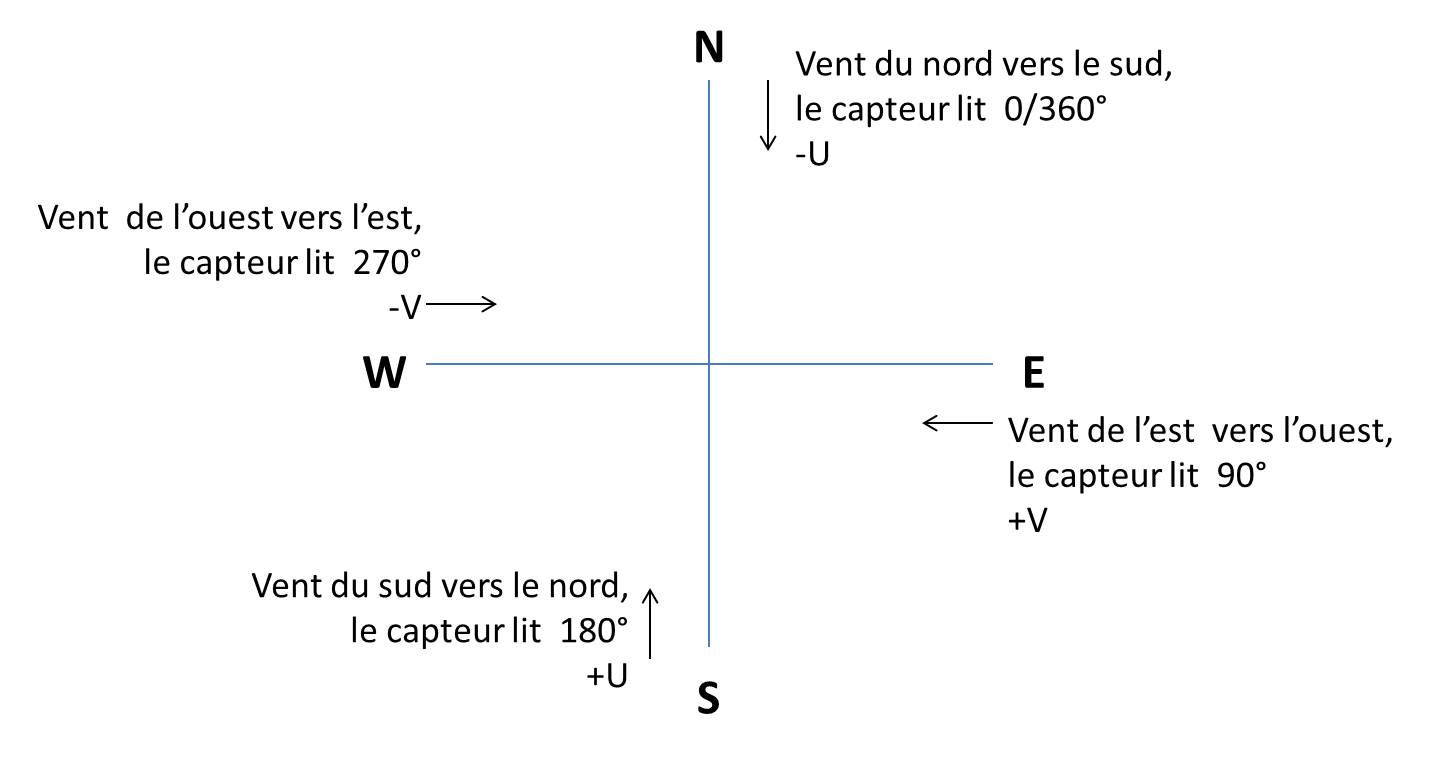
\includegraphics[width=14cm]{WindSonic3.jpg}
		\caption{Correspondance entre les valeurs mesur�es, la direction du vent et la polarit� UV.}
		\label{Fig.7}
	\end{figure}

\subsection{Positionnement du capteur}
Idem 10.2

\subsection{Maintenance du capteur}
Idem 10.3

\subsection{Calibration et d�rive du capteur}
Idem 10.4

\subsection{Informations compl�mentaires}
La direction du vent n'est pas calcul�e pour les vitesses de vent inf�rieures � 0.05 m.s$^{-1}$ et la valeur de direction restera bloqu�e sur la derni�re valeur mesur�e jusqu'� qu'une nouvelle direction puisse �tre calcul�e.

\newpage

\section{Humidit� relative de l'air - RH - HUMICAP(r) (HMP155A)}

\subsection{Principe de mesure et unit�}
Le capteur d'humidit� se situe dans la sonde HMP155A qui mesure �galement la temp�rature (cf section 5)

La mesure de l'humidit� est r�alis�e par un capteur capacitif constitu� d'un film fin de polym�re HUMICAP(r) (3 dans Fig. 2). Le capteur contient un condensateur dont le di�lectrique est sensible � l'humidit�. Le capteur HMP155A mesure l'humidit� relative de l'air sur une gamme allant de 0 � 100\%.

L'unit� est le pourcentage de saturation en eau de l'air, \%. 


\subsection{Positionnement du capteur}
Idem 5.2.

\subsection{Maintenance du capteur}
Le capteur d'humidit� HUMICAP(r) peut �tre chang�:
	\begin{enumerate}
		\item Enlever le filtre de la sonde.
		\item V�rifier le joint torique, le changer si n�cessaire.
		\item enlever le capteur d�fectueux (3 dans Fig. 2) et le remplacer par un nouveau. ATTENTION : manipuler le nouveau capteur en le laissant dans son plastique, IL NE FAUT PAS TOUCHER LE CAPTEUR.
		\item calibrer le capteur
		\item mettre un nouveau filtre.
	\end{enumerate}
	
Pour la maintenance de la sonde, voir 5.3.

\subsection{Calibration et d�rive du capteur}
Le capteur HUMICAP(r) de la sonde HMP155A est calibr� par le fabricant. Il est recommand� de renouveler la calibration tous les ans et que celle-ci soit r�alis�e par Vaisala (voir www.vaisala.com/returns).

Cependant, la calibration peut �tre r�alis�e au laboratoire dans la condition standard de tempr�ature ($25\,^{\circ}\mathrm{C}$)avec la m�thode de la solution en sel satur�e. Une solution de sel satur� dans un container �tanche � l'air a la propri�t� de maintenir une humidit� de l'air approximativement constante. L'humidit� atteinte d�pend de la nature du sel: 11\% pour LiCl$_2$, 33\% pour MgCl$_2$, 43\% pour K$_2$CO$_3$, 75\% pour NaCl$_2$ et 97\% pour K$_2$SO$_4$. Les deux humidit�s relatives de calibration doivent avoir une diff�rence d'au moins 30\%. La calibration peut se faire avec deux point de mesure comme suit:
	\begin{enumerate}
		\item Acc�der aux boutons d'ajustement en d�vissant le capuchon de protection (1 dans la Fig. 3) et le scell� de calibration.
		\item relever le couvert de protection (5 dans la Fig. 3)pour voir les boutons d'ajustement (2, 3 et 4 dans la Fig. 3). Il y a �galement une LED � 2 couleurs.
		\item Presser le bouton d'ajustement ADJ (celui correspondant au rectangle, 3 dans la Fig. 3) jusqu'� que la LED s'allume en vert. La sonde HMP155A est alors en mode calibration.
		\item Enlever le filtre et ins�rer la sonde dans une chambre contenant la solution de calibration "s�che" (e.g. LiCl$_2$). ATTENTION : ne pas toucher le bouton d'ajustement avant la stabilisation des conditions. Cela peut prendre environ 30 minutes.
		\item En utilisant les boutons + et -, r�aliser l'ajustement du gain pour l'humidit� basse pour s'assurer que le voltage A$_{out}$ est correct, puis appuyer sur le bouton ADJ. La LED verte s'�teint puis se rallume.
		\item Ins�rer la sonde dans une chambre contenant la solution de calibration "humide" (e.g. NaCl$_2$). ATTENTION : ne pas toucher le bouton d'ajustement avant la stabilisation des conditions. Cela peut prendre environ 30 minutes.
		\item En utilisant les boutons + et -, r�aliser l'ajustement du gain pour l'humidit� haute pour s'assurer que le voltage A$_{out}$ est correct. Pour finir la calibration, presser le bouton ADJ et la LED rouge s'allume.
		\item Presser ensuite le bouton ADJ 2 fois et la lumi�re s'�teint. La sonde HMP155A quitte ainsi le mode calibration.
	\end{enumerate}

La d�rive du capteur sur le terrain peut �tre suivie au moins une fois tous les 6 mois en effectuant le m�me mode op�ratoire que la calibration, mais sans r�aliser les ajustements (ne pas mettre le capteur en mode calibration), c'est � dire en pla�ant la sonde dans des containers contenant diff�rentes solutions salines satur�es et en r�alisant une lecture simple de l'humidit� de l'air des containers.

\newpage

\section{Temp�rature de l'air - Ta - Pt100 (HMP155A)}

\subsection{Principe de mesure et unit�}
Le capteur de temp�rature se situe dans la sonde HMP155A qui mesure �galement l'humidit� relative (cf section 6)

La mesure de la temp�rature est r�alis�e par un thermom�tre � r�sistance de platine (Pt100, 4 dans Fig. 2). Le principe de mesure de ce capteur est bas� sur le fait que la r�sistivit� �lectrique du platine varie avec la temp�rature.

La sonde HMP155A mesure la temp�rature de l'air sur une gamme allant de $-80\,^{\circ}\mathrm{C}$ � $+60\,^{\circ}\mathrm{C}$.

L'unit� est de d�gr� Celsius, $^{\circ}\mathrm{C}$. 
	
	\begin{figure}[h] 
		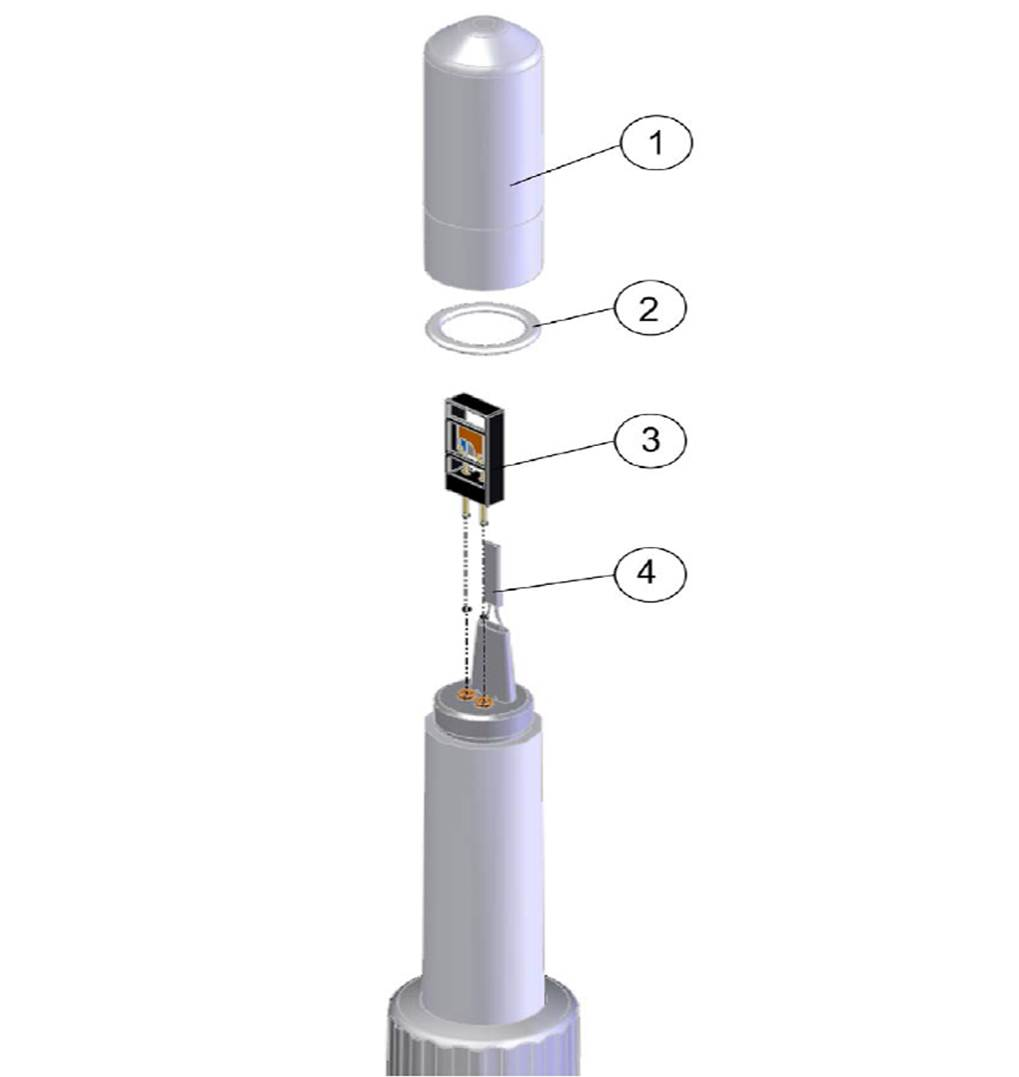
\includegraphics[width=8cm]{HMP155A_bis.jpg}
		\caption{Les capteurs de la sonde HMP155A: 1 = filtre, 2 = joint torique, 3 = capteur d'humidit� HUMICAP(r), 4 = capteur de temp�rature Pt100.}
		\label{Fig.2}
	\end{figure}

\subsection{Positionnement du capteur}
La sonde HMP155A doit �tre install� dans un abri de type DTR13 (possibilit� d'ajouter une sonde de temp�rature suppl�mentaire) ou DTR503.

L'ensemble capteur et abri doivent �tre plac� dans une zone ouverte correspondant � une surface de 9 m de diam�tre. La temp�rature de l'air intervient dans l'�quation de Penman-Monteith pour calcul de l'�vapotranspiration. Cette �quation a pour pr�suppos� que toutes les mesures des variables intervenant dans l'�quation sont r�alis�es � 2 m au dessus de la surface du sol. Le capteur de temp�rature seront donc dispos� � une hauteur de 2 m au dessus de la surface de chaque tourbi�re.

\subsection{Maintenance de la sonde}
Si la sonde doit �tre nettoy�, utilisez un chiffon non-pelucheux mouill� avec un d�tergent relativement faible.

Si le filtre reste sale apr�s le nettoyage, il faut le remplacer. V�rifiez que le joint torique est encore en bon �tat, sinon, changez-le.

\subsection{Calibration et d�rive du capteur}
Le capteur Pt100 de la sonde HMP155A est calibr� par le fabricant. Il est recommand� de renouveler la calibration tous les ans et que celle-ci soit r�alis�e par Vaisala (voir www.vaisala.com/returns).

Cependant, la calibration peut �tre r�alis�e au laboratoire en utilisant une enceinte capable de r�guler la temp�rature (e.g. phytotron). Les deux temp�ratures de calibration doivent avoir une diff�rence d'au moins $30\,^{\circ}\mathrm{C}$. La calibration peut se faire comme suit:
	\begin{enumerate}
		\item Acc�der aux boutons d'ajustement en d�vissant le capuchon de protection (1 dans la Fig. 3) et le scell� de calibration.
		\item relever le couvert de protection (5 dans la Fig. 3)pour voir les boutons d'ajustement (2, 3 et 4 dans la Fig. 3). Il y a �galement une LED � 2 couleurs.
		\item Presser le bouton d'ajustement ADJ (celui correspondant au rectangle, 3 dans la Fig. 3) jusqu'� que la LED s'allume en vert. La sonde HMP155A est alors en mode calibration.
		\item Enlever le filtre et ins�rer la sonde dans une enceinte dont la temp�rature est connue et laisser la lecture se stabiliser. ATTENTION : ne pas toucher le bouton d'ajustement avant la stabilisation des conditions.
		\item En utilisant les boutons + et -, r�aliser l'ajustement de la temp�rature en s'assurant que le voltage A$_{out}$ est correct, puis appuyer sur le bouton ADJ. La LED verte s'�teint puis se rallume.
		\item Ins�rer la sonde dans une enceinte dont la temp�rature est diff�rente de la premi�re et laisser le temp�rature se stabiliser. ATTENTION : ne pas toucher le bouton d'ajustement avant la stabilisation des conditions.
		\item En utilisant les boutons + et -, r�aliser l'ajustement de la temp�rature en s'assurant que le voltage A$_{out}$ est correct. Pour finir la calibration, presser le bouton ADJ et la LED rouge s'allume.
		\item Presser ensuite le bouton ADJ 2 fois et la lumi�re s'�teint. La sonde HMP155A quitte ainsi le mode calibration.
	\end{enumerate}
	

	\begin{figure}[h] 
		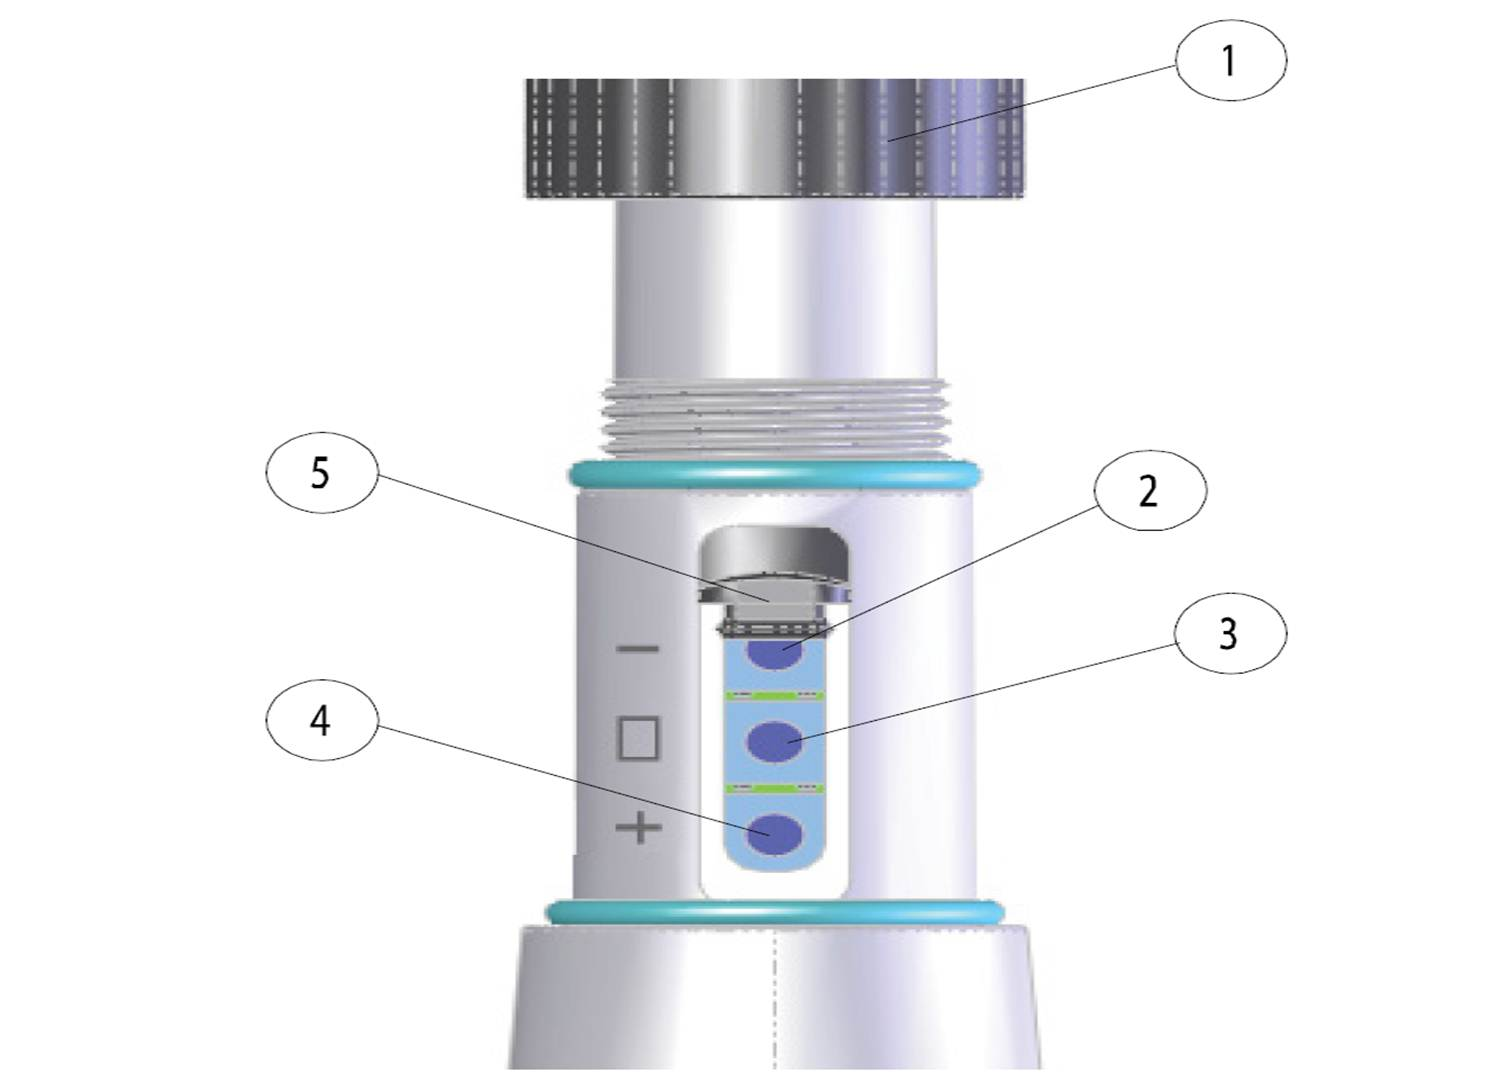
\includegraphics[width=10cm]{HMP155A_ter.jpg}
		\caption{Les boutons d'ajustements pour la calibration des capteurs de la sonde HMP155A: 1 = capuchon de protection (d�viss�e), 2 = bouton pour diminuer, 3 = bouton ADJ, 4 = bouton pour augmenter, 5 = couvert de protection des bouton relev�.}
		\label{Fig.3}
	\end{figure}

La d�rive du capteur sur le terrain peut �tre suivie au moins une fois tous les 6 mois en effectuant des mesures de temp�ratures au m�me endroit et dans les m�me conditions avec un autre capteur (un autre HMP155A, une autre marque, voir un thermom�tre � mercure).

\subsection{Informations diverses}
Le capteur consomme moins de 3 mA (courant � 12 V). Deux secondes de mise en chauffe sont n�cessaires. Pour des vitesses d'acquisition plus lentes qu'une mesure toutes les 5 secondes, la sonde peut �tre commut�e pour �conomiser la batterie.

\newpage

\section{Temp�rature du sol - Ts - 107}

\subsection{Principe de mesure et unit�}
La sonde 107 utilise un thermistor pour mesurer la temp�rature. Un thermistor est une r�sistance dont la r�sistance est fonction de la temp�rature. Cette relation n'�tant lin�aire que sur une faible gamme de temp�rature, l'�quation de Steinhart-Hart est pr�f�r�e (polynome d'ordre 3). Dans le pire des cas, la pr�cision atteind +/- 0.4�C sur la gamme -24�C - 48�C.

La sonde applique une tension d'excitation V$_x$ de 2500 mV � un thermistor de 1 kohm et mesure la chute de tension (tension mesur�e V$_s$). La r�sistance R$_s$ est calcul�e de la mani�re suivante:
		\begin{equation}
		V_s/V_x = 1000 /  (R_s + 249000 + 1000)
		\end{equation} 
		
Ensuite, la r�sistance R$_s$ est convertie en temp�rature (�C) avec l'�quation de Steinhart-Hart:
		\begin{equation}
		T = 1 /  (A + B(LnR_s) + C(LnR_s)^3) - 273.15
		\end{equation}
Avec:

\

A = 8.271111 x 10$^{-4}$

\

B = 2.088020 x 10$^{-4}$

\

C = 8.059200 x 10$^{-8}$
		

\subsection{Positionnement du capteur}
La position des capteurs de physique du sol sont d�crits dans la section ??.

\subsection{Maintenance du capteur}
La 107  n'a pas besoin d'une maintenance p�riodique.

\subsection{Calibration et d�rive du capteur}
Il n'est pas n�cessaire de faire de calibration.

\newpage

\section{Teneur en eau du sol - SWC - CS650}

\subsection{Principe de mesure et unit�}
La sonde CS650 est une sonde multiparam�tre permettant de mesurer la teneur volum�trique en eau, la conductivit� �lectrique, la permittivit� di�lectrique et la temp�rature du sol dans lequel elle est plac�e. 

La sonde est compos�e de 2 broches en acier inoxydable de 30 cm de longueur. La mesure est bas�e sur la sensibilit� du capteur � la permittivit� di�lectrique du milieu entourant les broches. La teneur en eau est le principal facteur d�terminant la permittivit� di�lectrique d'un milieu. Apr�s une calibration, il est possible d'estimer une teneur en eau � partir de la permittivit� di�lectrique.

La sonde CS650 est configur�e de mani�re a fonctionner comme un r�flectom�tre, avec les 2 broches formant une ligne de transmission ouverte en partie terminale. Un signal �lectrique est �mis, puis il est r�fl�chit lorsqu'il arrive au bout de la broche et il revient � son point initial. La vitesse � laquelle l'onde �lectromagn�tique effectue l'aller-retour varie en fonction de la permittivit� �lectrique du mat�riau atour du capteur. La permittivit� augmente avec l'augmentation de la teneur en eau et diminue avec la diminution de la teneur en eau. La permittivit� est mesur� en Farad par m�tre (F m$^{-1}$).

La conductivit� �lectrique est mesur�e en excitant une broche avec une onde de fr�quence connue et en mesurant l'att�nuation du signal. Elle est exprim�e en Siemens par m�tre (S m$^{-1}$).

La temp�rature est mesur�e avec une thermistance en contact avec une des broches. Elle est exprim�e en degr� Celsius (�C).

Une fois calibr�, la sonde peut donner des valeurs de teneur en eau du sol en mm$^3$ par mm$^3$.

\subsection{Variable de sortie}
Le capteur CS650 donne 6 variables de sorties:

	\begin{enumerate}
		\item Volumetric Water Content : VWC
		\item Bulk Electrical Conductivity : EC (dS/m)
		\item Soil temperature
		\item Bulk Dielectric Permittivity : Ka
		\item Period Average : PA ($�$s)
		\item Voltage Ratio : VR	
	\end{enumerate}

Ces variables de sorties seront stock�es dans le dossier "Data brutes" plac� sur le serveur ftp SNO Tourbi�res de l'OSUC. ATTENTION: la teneur en eau donn�e par la sonde est indicative, mais elle n'est pas correcte, parce qu'elle a �t� calcul�e avec une courbe de calibration estim�e avec des sols min�raux.


\subsection{Positionnement du capteur}
La position des capteurs de physique du sol sont d�crits dans la section ??.

\subsection{Maintenance du capteur}
La sonde CS650  n'a pas besoin d'une maintenance p�riodique.

\subsection{Calibration}
L'�quation de calibration utilis�e par la sonde CS650 est l'�quation de Topp et al. (1980). Cette �quation marche bien pour les sols min�raux, mais sous-estime les teneurs en eau pour les sols organiques volcaniques et � fines textures. Dans le cadre du SNO, une calibration doit �tre r�alis�es pour obtenir une calibration sp�cifique. Elle permettra de relier les valeur de permittivit� � la teneur en eau mesur�e par une une m�thode ind�pendante.

Cette �quation peut-�tre une �quation lin�aire ou quadratique ou un polynome d'ordre 3. Ces �quations ont besoin d'un minimum de 2, 3 et 4 points de calibration, respectivement. Ces points doivent �tre choisis de mani�re � couvrir toute la gamme de valeur de teneur en eau: basses eaux, hautes eaux et interm�diaires.

La teneur en eau des �chantillons pr�lev� sur le terrain sera mesur�e par gravim�trie au laboratoire selon le protocole suivant:

	\begin{enumerate}
		\item A proximit� du profil de teneur en eau, une tranch�e est creus�e avec un front de taille "propre". 
		\item Ensuite, avec un cylindre en fer de volume V et de masse connus, un �chantillon est pr�lev� horizontalement dans le front de taille. 
		\item 3 r�plicats par profondeur sont pr�lev�s (grande variabilit� spatiale, surtout en surface).
		\item Cette op�ration est r�p�t�es pour chaque profondeur o� se trouve une CS650.
		\item Le cylindre contenant l'�chantillon est sc�ll� � ces extr�mit�s pour ne pas perdre de l'eau.
		\item Au laboratoire,l'�chantillon humide est pes�: m$_humide$ (tourbe humide + cylindre).
		\item L'�chantillon est plac� dans une �tuve � 105�C.
		\item Apr�s 48 heures � l'�tuve, l'�chantillon est pes� de nouveau: m$_sec$ (tourbe s�che + cylindre).
		\item La teneur en eau massique SWC$_m$ vaut: 
				\begin{equation}
				SWC_m = m_{humide} - m_{sec} /  m_{sec}
				\end{equation}
		\item La densit� apparente vaut: 
				\begin{equation}
				\rho _{bulk} = m_{sec} / V
				\end{equation}	
		\item La teneur en eau volumique SWC$_v$ vaut: 
				\begin{equation}
				SWC_v = SWC_m * \rho _{bulk}
				\end{equation}
				
	\end{enumerate}
	
Cette mesure de teneur en eau correspond � la variable obligatoire #49 "teneur en eau du sol, manuel" du tableau 1.3. Ces donn�es seront stock�es dans un fichier plac� dans le dossier "Data corrig�es". Les param�tres de la courbe de calibration seront stock�s dans un fichier log situ� dans le dossier "Log2". Une fois les param�tres de la courbe calcul�s, les teneurs en eau du sol pourront �tre calcul�es et stock�es dans un fichier contnu dans le dossier "Data corrig�es". Cette valeur correspond � la variable # 9 du tableau 1.3, "Teneur en eau du sol".
	

\subsection{Informations diverses}
Les broches des CS650 font 30 cm de longueur. Cette taille permet d'�chantillonner un grand volume de sol et d'avoir par cons�quent une r�duction de l'erreur de mesure. Le volume �chantillonn� s'�tend � 7.5 cm autour des broches et 4.5 cm au del� de la fin des broche. Le volume total �chantillonn� est de 7800 cm$^3$. 

\newpage

\section{Flux de chaleur dans le sol - G - Hukseflux}

\subsection{Principe de mesure et unit�}

\subsection{Positionnement du capteur}

\subsection{Maintenance du capteur}

\subsection{Calibration et d�rive du capteur}

\newpage

\section{Niveau de la nappe d'eau - GWL - CS451}

\subsection{Principe de mesure et unit�}
La mesure de niveau est r�alis�e � partir d'une mesure automatis�e et fr�quente de pression de la colonne d'eau sur le capteur situ� dans le pi�zom�tre et d'une mesure manuelle du niveau de la colonne d'eau. La pression de la colonne d'eau mesur� est corrig� en soustrayant la presison atmosph�rique �galement enregistr�e par le capteur.

\subsection{Positionnement du capteur}
Le capteur est situ� dans un pi�zom�tre cr�pin�. Celui-ci doit collecter seulement les eaux de la tourbi�re (attention, parfois un forage trop profond per�ant une nappe sous-jacente induit des mesures erron�es).

\subsection{Maintenance du capteur}
Inspecter visuellement le c�blage, v�rifier le dessicant, le remplacer si n�cessaire.

\subsection{Calibration et d�rive du capteur}
Le fabricant recommande une recalibration tous les 2 ans.

\newpage

\section{Positionnement des capteurs}

\subsection{Mesures dans le sol}
Le positionnement des sondes du sol correspond aux recommandations ICOS. Horizontalement, les sondes de temp�ratures et de teneurs en eau devront �tre dispos�es de part et d'autre de la sondes de flux de chaleur dans le sol et s�par�es de 30 cm au moins ou de 45 cm au plus (Fig. 3.7). Le pi�zom�tre dans lequel sera install� la sonde de niveau d'eau se trouvera � 2 m de la sonde de flux de chaleur dans le sol (Fig. 3.7) 

\

	\begin{figure}[h] 
		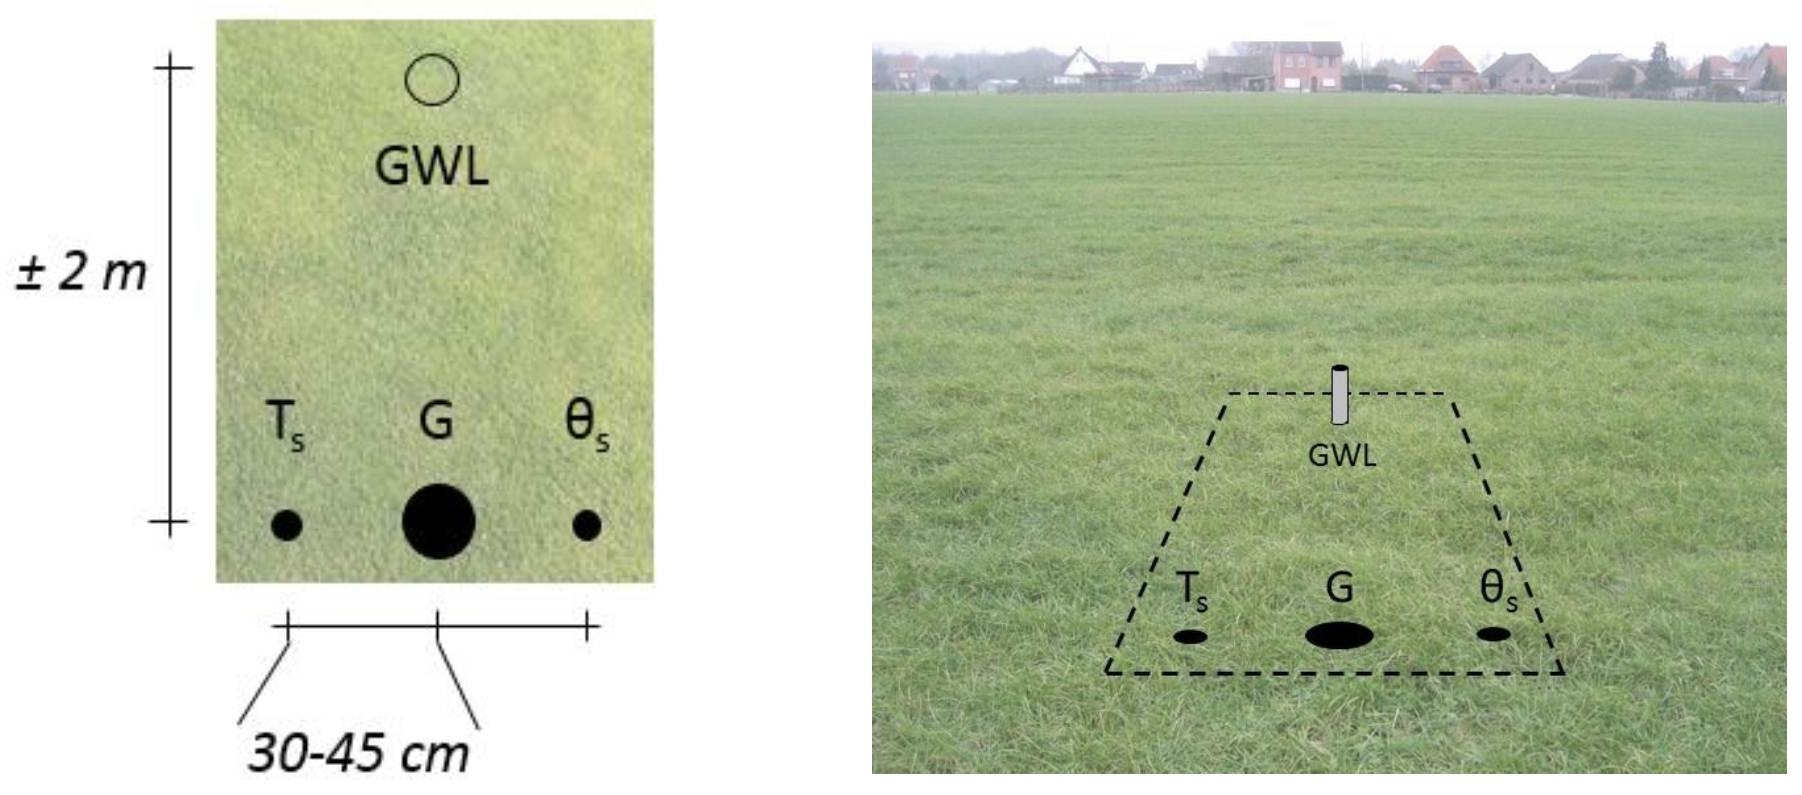
\includegraphics[width=14cm]{sonde_sol_horizontal.jpg}
		\caption{Distribution horizontale des sondes du sol (protocole ICOS, 2015).}
		\label{Fig.4}
	\end{figure}

\

Pour les sites ICOS de niveau 2, au moins deux plots de mesures doivent �tre install�s. Dans chaque plot, deux profils sont mis en place : un profil complet et un profil additionnel pour prendre en compte la variabilit� spatiale des variables mesur�es, notamment celle du flux de chaleur dans le sol.

Pour le profil complet, seront install�es (Fig. 3.8 a): 

	\begin{itemize}
		\item 5 sondes de temp�ratures : -2 cm, -5 cm, -10 cm, -25 cm et -60 cm,
		\item 3 sondes de teneur en eau du sol : -5 cm, -10 cm et -25 cm,
		\item 1 sonde de flux de chaleur dans le sol : -5 cm,
		\item une sonde du niveau de la nappe d'eau.
	\end{itemize}	
		
Des ajustements peuvent �tre fait selon les contraintes de chaque sites. Dans tous les cas, les profondeurs devront �tre not�es dans le fichier log des variables (cf chapitre 1, dossier Log 1). La derni�re sonde de temp�rature devrait �tre install�e en dessous du niveau de nappe le plus bas. Les sondes ne sont pas n�cessairement align�es. Il serait pr�f�rable de les install�es en diagonale.

Pour le profil additionnel, seront install�es (Fig. 3.8 b) : 

	\begin{itemize}
		\item 3 sondes de temp�ratures : -2 cm, -5 cm et -10 cm, 
		\item 1 sondes de teneur en eau du sol : -5 cm,
		\item 1 sonde de flux de chaleur dans le sol : -5 cm,
	\end{itemize}	


\

	\begin{figure}[h] 
		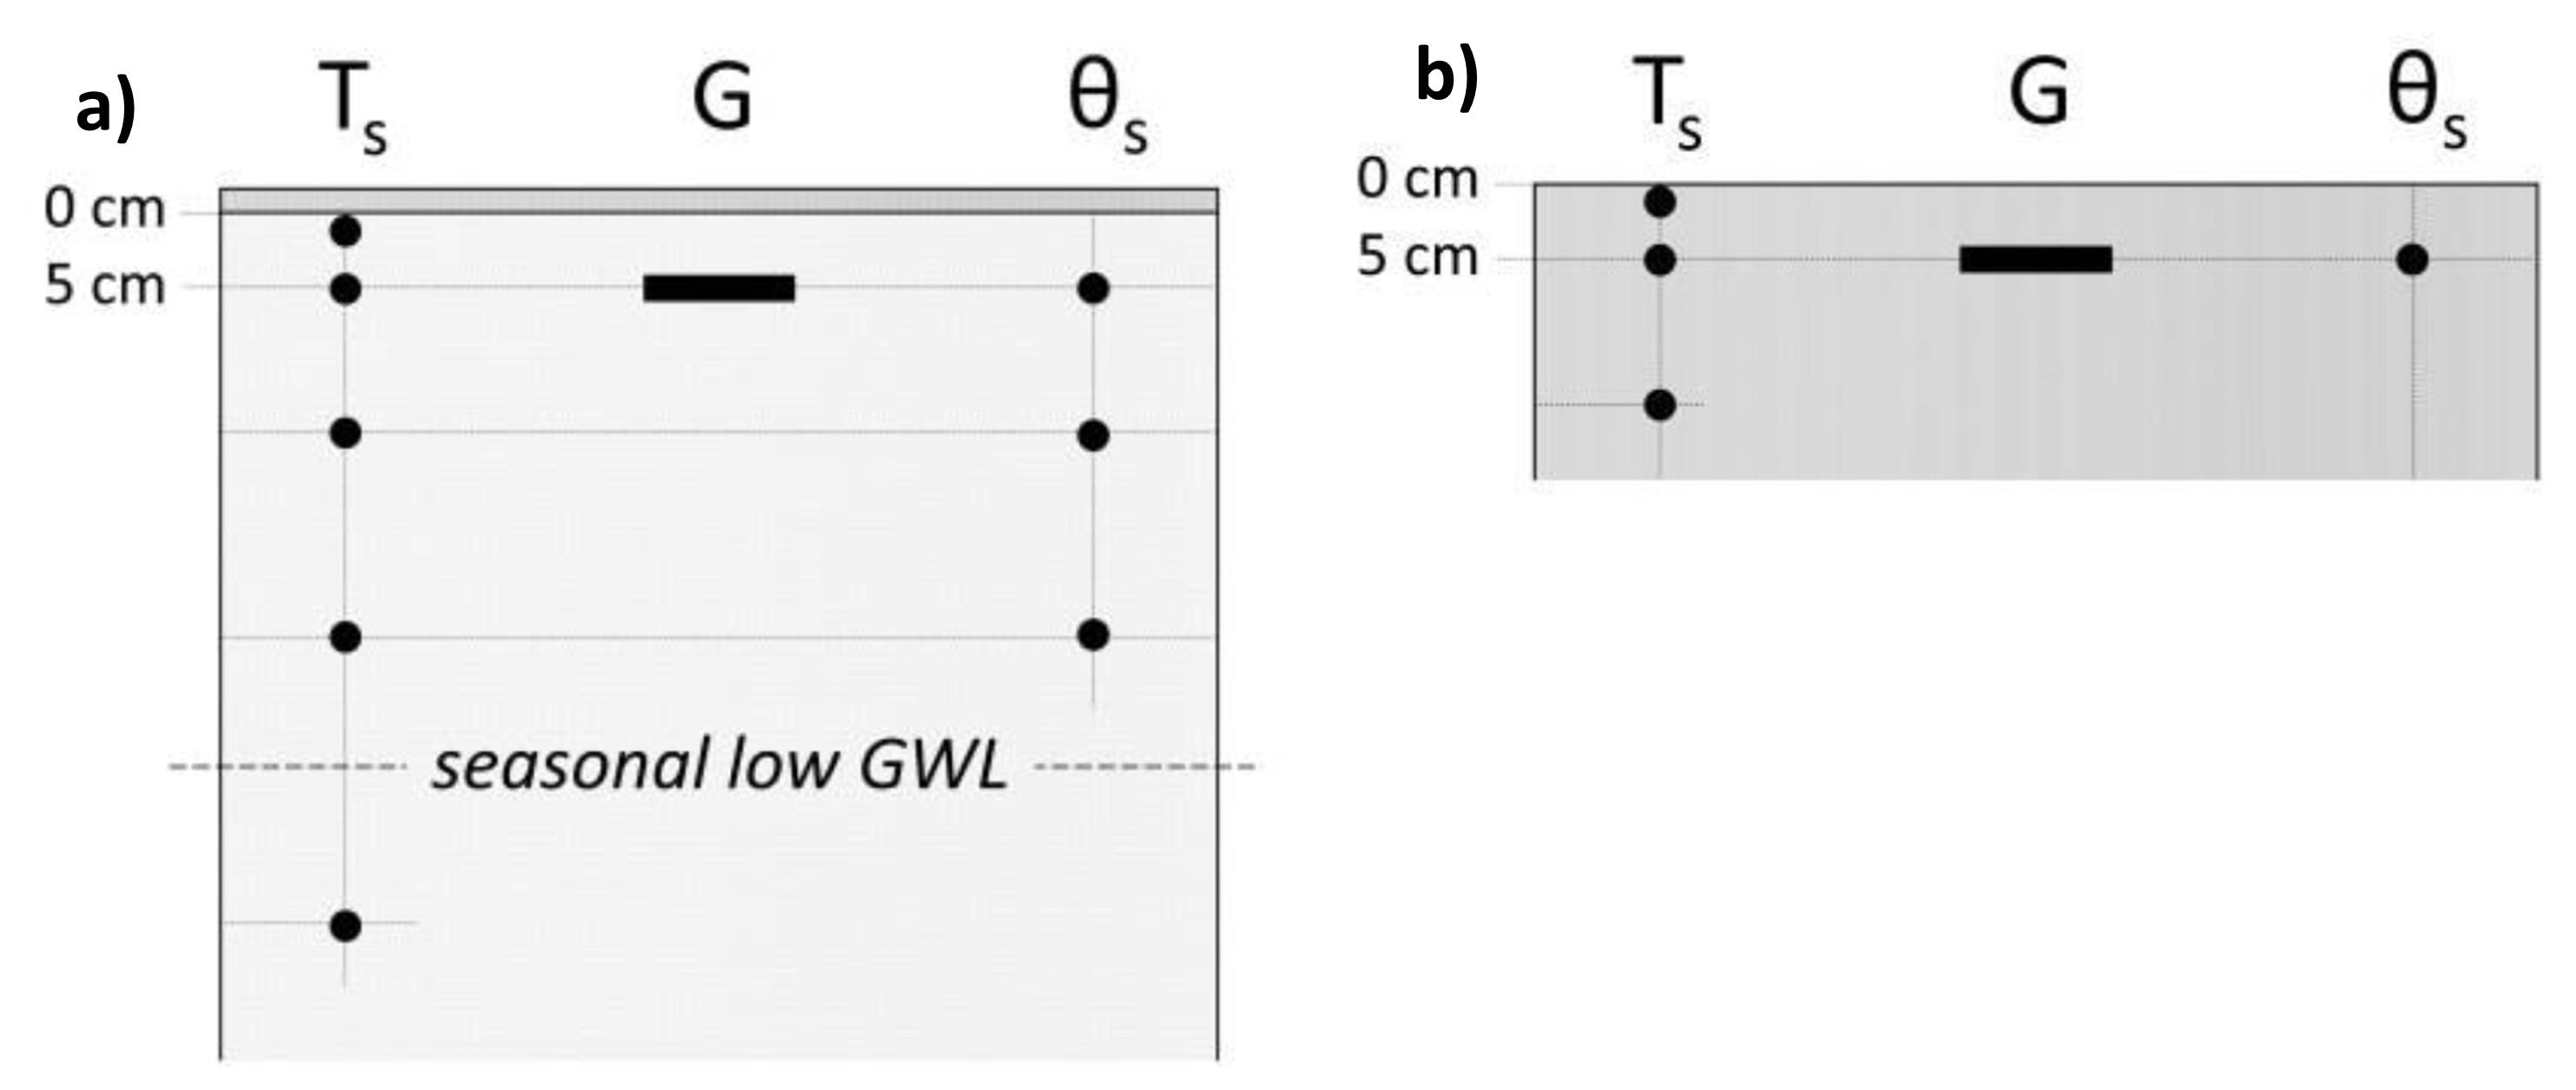
\includegraphics[width=14cm]{profil_sol.jpg}
		\caption{Distribution verticale des sondes du sol dans le profil complet (a) et additionnel(b; protocole ICOS, 2015).}
		\label{Fig.5}
	\end{figure}

\



\subsection{Mesures dans l'atmosph�re}



\newpage

\section{Bibliographie}


		
\newpage

		%--- CHAPITRE 4: Hydrologie
		
%---------------- %   Chapitre 4   %--------------- %


% % % % % % % % % % % % % % % % % % % % % % % % % % %
%													%	
%			 SNO Tourbi�res - Hydrologie			%
%													%	
% % % % % % % % % % % % % % % % % % % % % % % % % % % 





\chapter{Hydrologie}

S. Gogo, S. Binet, L. Bernard-Jannin...

\section{Cadre et objectif des mesures}
Les tourbi�res �tant des zones humides, la connaissance de leur fonctionnement hydrologique est essentielle pour comprendre le syst�me dans sa globalit�. Les mesures du niveau de la nappe d'eau (ou Ground Water Level, GWL) et du d�bit � l'exutoire sont les variables obligatoires pour comprendre ce fonctionnement. Coupl�es avec des mesures m�t�orologiques, elles permettent l'�tablissement du bilan hydrique. De plus, l'hydrologie, en influen�ant la teneur en eau du sol, va d�terminer l'intensit� des processus biog�ochimiques � l'origine des flux de GES: la respiration s'effectue de mani�re optimale dans une gamme de teneur en eau volumique du sol d'environ 30 � 80 \% et la m�thanog�n�se ne s'effectue qu'en conditions ana�robique. Dans ce cas, la profondeur de la nappe d'eau (Ground Water Depth, GWD) est la variable la plus indiqu� car elle informe de l'�paisseur de la zone a�robique.


\textbf{Les objectifs de ces mesures sont:}

\

		\begin{itemize}
			\item \textbf{D�terminer le bilan hydrique de chaque site}
			
			\
			
			\item \textbf{Fournir des donn�es pour calibrer/valider des mod�les hydrologiques}
			
			\
			
			\item \textbf{Fournir des donn�es pour calibrer/valider des mod�les de flux de GES}

		\end{itemize}

%\newpage




\section{Organisation des �quipements}

\subsection{Nombre de stations d'acquisition}

\paragraph{Stations intra-tourbi�re} Dans chaque site, en dehors des profils m�t�o-sol, au moins un pi�zom�tre �quip� d'un capteur automatique est demand�. Cette station est not�e \#006. Au maximum, 10 pi�zom�tres intra-tourbi�res (en dehors des profils m�t�o-sol) peuvent �tre install�s et seront not�s de \#007 � \#015. Les donn�es provenant de ces stations permettront d'�valuer le stock d'eau dans la tourbi�re et ses variations.


\paragraph{Stations exutoire} La mesure du d�bit � haute fr�quence � l'exutoire est estim� gr�ce � une courbe de tarage (relation entre le niveau de l'eau � l'�xutoire et le d�bit) et la mesure en � haute fr�quence du niveau de l'eau � l'exutoire. Une station d'acquisition avec sa sonde peut �tre install�e, mais en fonction des caract�ristique du site, plusieurs sondes peuvent �tre utilis�es (e.g. cas de Landemarais) avec au maximum 5 sondes. Ces stations seront not�es de \#016 � \#020.


%\newpage

\section{Les variables}

\subsection{Liste et abr�viations des variables cibles}
Les variables cibles concern�es par ce chapitre sont:

	%\textbf{code variable:}
		\begin{itemize}	
			\item 	\textbf{GWL} = niveau de la nappe d'eau dans la tourbi�re par rapport � une r�f�rence fixe (ground water level)
			\item 	\textbf{GWD} = niveau de la nappe d'eau par rapport au haut des sphaignes (ground water depth) 
			\item 	\textbf{Q} = d�bit � l'�xutoire
		\end{itemize}
		
Pour rappel, les d�tails des informations concernant les noms de fichier, le type de variables et leur code sont disponibles dans le chapitre 1.

\subsection{D�finition}
\paragraph{Le niveau de la nappe d'eau} Cette variable est l'altitude de la surface de la nappe d'eau libre (GWL dans Fig 4.1). Elle est calcul� en connaissant l'altitude d'un point de r�f�rence not� A$_{ref}$ sur la figure 4.1 (e.g. point IGN), en y soustrayant la distance entre le capteur de pression et le point de r�f�rence (not� L sur la figure 4.1) et en ajoutant l'�paisseur de la lame d'eau mesur�e entre le capteur et le haut de la nappe (not� H sur la figure 4.1). Un point IGN �tant tr�s rarement disponible aupr�s de la tourbi�re, un autre point de r�f�rence dont il faudra estimer l'altitude et dont on s'assura qu'il ne fluctue pas pourra servir de r�f�rence.

	\begin{figure}[h] 
		\centering
		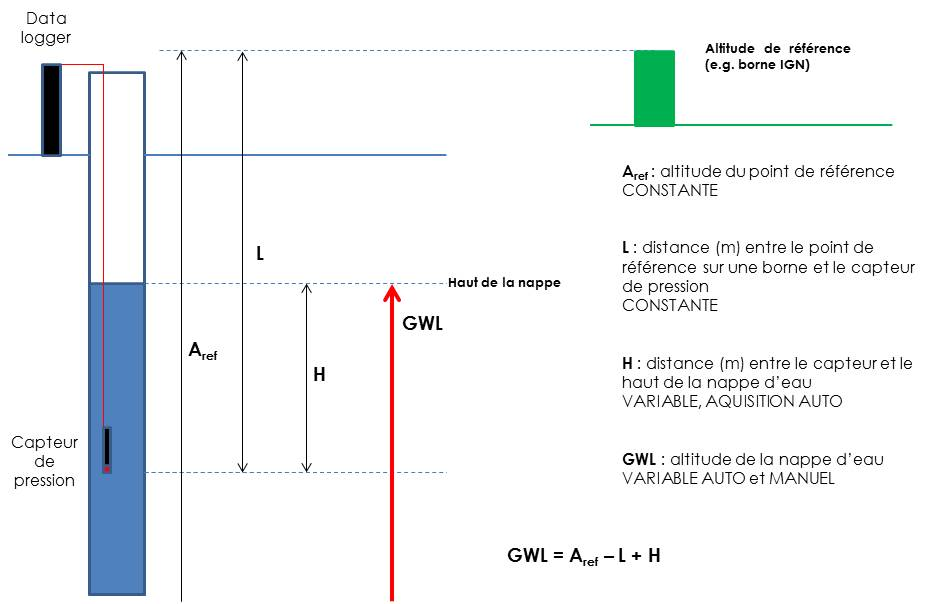
\includegraphics[width=14cm]{hydro_1.jpg}
		\caption{Sch�ma des mesures permettant d'obtenir des niveaux de la nappe d'eau.}
		\label{Fig. hydro 1}
	\end{figure}
	
\paragraph{La profondeur de la nappe d'eau} Cette variable est la distance alg�brique entre le haut des sphaignes (ou la surface du sol quand il n'y a pas de sphaignes) et la surface de la nappe d'eau libre (GWD dans Fig 4.2). Elle est positive quand l'eau est au dessus des sphaignes . Elle est n�gative quand l'eau est en dessous des sphaignes (cas le plus fr�quent). Pratiquement, le pi�zom�tre d�passe du tapis de sphaignes et lors des mesures manuelles, 2 mesures sont r�alis�es: 1) la distance entre le haut du pi�zom�tre et la nappe d'eau(d$_{nappe}$ dans Fig 4.1) et 2) la distance entre le haut du pi�zom�tre et le haut des sphaignes (d$_{ref}$ dans Fig 4.1)). La diff�rence donne la profondeur de nappe (GWD$_{manuel}$). Le capteur mesure l'�paisseur de la tranche d'eau (H, Fig. 2). De la distance L (Fig. 2) entre le haut du pi�zom�tre et le capteur, on retranche l'�paisseur H et d$_{ref}$ pour obtenir la GWD automatique.

	\begin{figure}[h] 
		\centering
		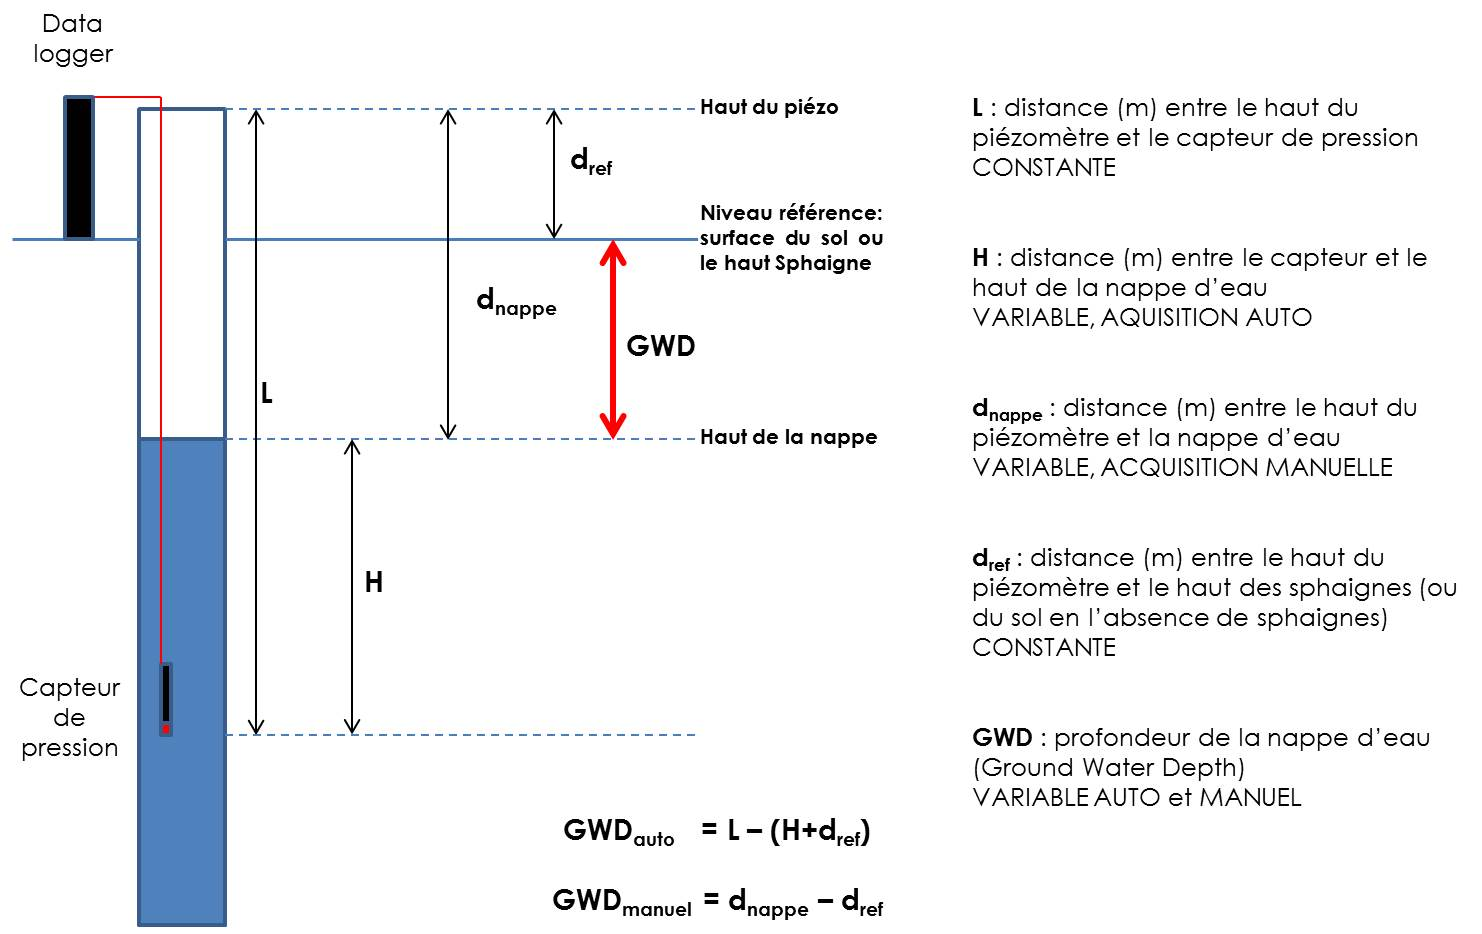
\includegraphics[width=14cm]{hydro_2.jpg}
		\caption{Sch�ma des mesures permettant d'obtenir des niveaux de la nappe d'eau.}
		\label{Fig. hydro 2}
	\end{figure}

\paragraph{Le d�bit � l'�xutoire} C'est le volume d'eau sortant � l'exutoire de la tourbi�re par unit� de temps. M�me si une sortie d'eau principale est g�n�ralement pr�sente, il existe le plus souvent de multiples sorties d'eau plus petites, du fait que les tourbi�res se d�veloppent en g�n�ral sur des zones plates. Les mesures de d�bit sont r�alis�es dans la sortie principale. 



\section{Le capteur de pression}

\subsection{Mod�les de capteurs}
Les membres du SNO Tourbi�res s'engage � tendre vers une uniformisation du parc analytique. Compte-tenu des contraintes inh�rente � chaque site et � la jouvence des appareils, cette uniformisation est th�orique. Cependant, le souci d'avoir des �quipements identiques doit �tre pr�sent pour une meilleur comparaison entre site et gestion des �quipements et des donn�es (un �quipement diff�rent dans chaque site pour une m�me variables implique des fournisseur diff�rents, avec des caract�ristiques techniques diff�rentes, des donn�es brutes diff�rentes, etc...). Pour rappel, la fr�quence d'acquisition est de une mesure toute les 30 minutes.

A ce jour, les capteurs les plus utilis�s sur nos sites sont les sondes OTT (mod�le Orpheus mini) et Schlumberger  (mod�le mini Diver). A l'�xutoire, la mesure de pression de la sonde EXO2 utilis�e pour le fluorescence et la turbidit� peut-�tre utilis�e si elle poss�de un capteur de pression.

\subsection{Principe de mesure et unit�}
La mesure du niveau d'eau est r�alis�e � partir d'une mesure de la pression hydrostatique de la colonne d'eau gr�ce � une cellule de pression relative. Pour les sondes OTT, la cellule de mesure dispose de la pression atmosph�rique via un tube capillaire localis� dans le c�ble de la sonde et  en contact avec l'air ambiant. Gr�ce � cette compensation, la sonde n'enregistre que les variations de pression li�es aux variations de la hauteur de la colonne d'eau. Pour les sondes Schlumberger, un capteur de pression atmosph�rique ind�pendant doit �tre install�.

Le niveau de la nappe d'eau est exprim�e en m�tre (m).

\subsection{Positionnement du capteur}
Pour les mesures intra-tourbi�res, un pi�zom�tre cr�pin� et bouch� � son extr�mit� inf�rieur est enfonc� dans la tourbe, si possible jusqu'au substratum. Il est important de s'assurer que le pi�zom�tre n'est pas connect� avec la nappe d'eau sous-jacente � la tourbi�re. Il est recommand� de recouvrir le haut du pi�zo avec un couvercle. La sonde de mesure de pression est plac�e dans le pi�zom�tre � un niveau suffisamment bas pour pouvoir enregistrer les niveaux de nappe pendant les s�cheresses. Des ajustement doivent �tre fait si le niveau d'eau descend en dessous du capteur et notifi� dans les dossier log.

S'il n'y a qu'une station d'acquisition, elle doit �tre plac�e au centre de la zone d'�tude. Si plusieurs station sont install�es, il recommand� de justifier leur emplacement dans les m�tadonn�es correspondantes.

Pour la mesure � l'exutoire, le capteur peut �tre install� dans un pi�zom�tre cr�pin� est plant� dans le lit du cours d'eau � l'�xutoire ou install� horizontalement. De m�me que pour les sondes dans la tourbi�re, le capteur de niveau d'eau � l'exutoire doit �tre capable d'enregistrer les s�cheresses.


\subsection{Maintenance du capteur}
A chaque collecte de donn�es, l'installation est v�rifi�e pour d�tecter tout probl�me apparent.

Des mesures aberrantes peuvent provenir d'une cellule de mesure encrass�e. Pour nettoyer le capteur de pressions, sortez le capteur du pi�zom�tre, d�vissez le bouchon de protection noir. Nettoyez avec pr�caution le capteur � l'eau avec un pinceau ou une brosse. Rincez abondamment avec de l'eau clair la sonde de pression, revissez le capuchon noir et replacez la sonde dans le tube. Si une telle maintenance est r�alis�e, elle doit �tre consign� dans le fichier log correspondant.

\section{Elaboration des variables cibles}

\subsection{Ground Water Level - GWL}
La variable mesur�e par le capteur est une hauteur de colonne d'eau (H dans Fig. 4.1). Pour conna�tre le niveau de la nappe d'eau GWL, il est n�cessaire de conna�tre la distance entre le capteur et un point de r�f�rence. Comme mentionn� plus haut, le haut des sphaignes sert de r�f�rence. Cette distance �tant variable, une r�f�rence interm�diaire est utilis�e: le haut du tube du pi�zom�tre. Le niveau de la nappe d'eau est calcul� en retranchant de la distance entre le haut du pi�zom�tre et la sonde (L sur le figure 4.1, mesur�e � l'installation de la sonde et constante), la distance entre le haut du pi�zom�tre et le haut des sphaignes et la hauteur de la colonne d'eau H (Fig. 4.1).

Certains de ces calculs peuvent �tre programm�s. Cependant, du fait de la croissance des v�g�taux, de l'accumulation de liti�re et du gonflement de la tourbe, une correction de la d�rive est souhaitable en r�alisant des mesures manuelles de niveau de la nappe d'eau (GWLm). Ce calcul �tant difficilement automatisable, il est r�alis�es par l'expert.

Dans la base de donn�es, les donn�es en sortie de capteur (H) sont inject�es au moins une fois par an dans le dossier "fichiers annuels" des dossiers "data brutes" des diff�rents sites (cf section 2.3.2) par l'expert responsable de l'hydrologie de chaque site (cf flux de donn�es 2.3.1, cas 2). Les donn�es de niveau de la nappe d'eau (GWL) sont plac�s dans le dossier "fichiers annuels" des dossiers "data corrig�es" des diff�rents sites (cf section 2.3.2). Les actions r�alis�es sur les donn�es brutes sont consign�es dans le log correspondant. Le nom des fichiers sera bas� sur la nomenclature d�crite au chapitre 1.


\subsection{Ground Water Depth - GWD}
La variable mesur�e par le capteur est une hauteur de colonne d'eau (H dans Fig. 4.1). Pour conna�tre le niveau de la nappe d'eau GWL, il est n�cessaire de conna�tre la distance entre le capteur et un point de r�f�rence. Comme mentionn� plus haut, le haut des sphaignes sert de r�f�rence. Cette distance �tant variable, une r�f�rence interm�diaire est utilis�e: le haut du tube du pi�zom�tre. Le niveau de la nappe d'eau est calcul� en retranchant de la distance entre le haut du pi�zom�tre et la sonde (L sur le figure 4.1, mesur�e � l'installation de la sonde et constante), la distance entre le haut du pi�zom�tre et le haut des sphaignes et la hauteur de la colonne d'eau H (Fig. 4.1).

Certains de ces calculs peuvent �tre programm�s. Cependant, du fait de la croissance des v�g�taux, de l'accumulation de liti�re et du gonflement de la tourbe, une correction de la d�rive est souhaitable en r�alisant des mesures manuelles de niveau de la nappe d'eau (GWLm). Ce calcul �tant difficilement automatisable, il est r�alis�es par l'expert.

Dans la base de donn�es, les donn�es en sortie de capteur (H) sont inject�es au moins une fois par an dans le dossier "fichiers annuels" des dossiers "data brutes" des diff�rents sites (cf section 2.3.2) par l'expert responsable de l'hydrologie de chaque site (cf flux de donn�es 2.3.1, cas 2). Les donn�es de niveau de la nappe d'eau (GWL) sont plac�s dans le dossier "fichiers annuels" des dossiers "data corrig�es" des diff�rents sites (cf section 2.3.2). Les actions r�alis�es sur les donn�es brutes sont consign�es dans le log correspondant. Le nom des fichiers sera bas� sur la nomenclature d�crite au chapitre 1.


\subsection{D�bit � l'�xutoire - Q}
Le d�bit est obtenu � partir de la relation qui le lie � la hauteur d'eau dans le canal de l'exutoire. Cette hauteur d'eau est enregistr�e � haute fr�quence. En r�alisant des mesures ponctuelles de d�bit et en mesurant simultan�ment la hauteur d'eau, on peu r�aliser une courbe de tarage qui permettra de transformer les hauteurs d'eau en d�bit.
La mesure de d�bit couramment employ�e dans le r�seau est la m�thode du d�bit au sel (Fig. 4.2). En amont d'un point de mesure ou la conductivit� �lectrique est mesur�, une masse connue de sel est inject� dans le cours d'eau. La conductivit� est enregistr�e � haute fr�quence. Une fois le panache de sel pass� (retour � une conductivit� de base), la mesure est stopp�e. L'int�gration de la conductivit� avec le temps donne une estimation du d�bit (Fig. 4.2).


	\begin{figure}[h] 
		\centering
		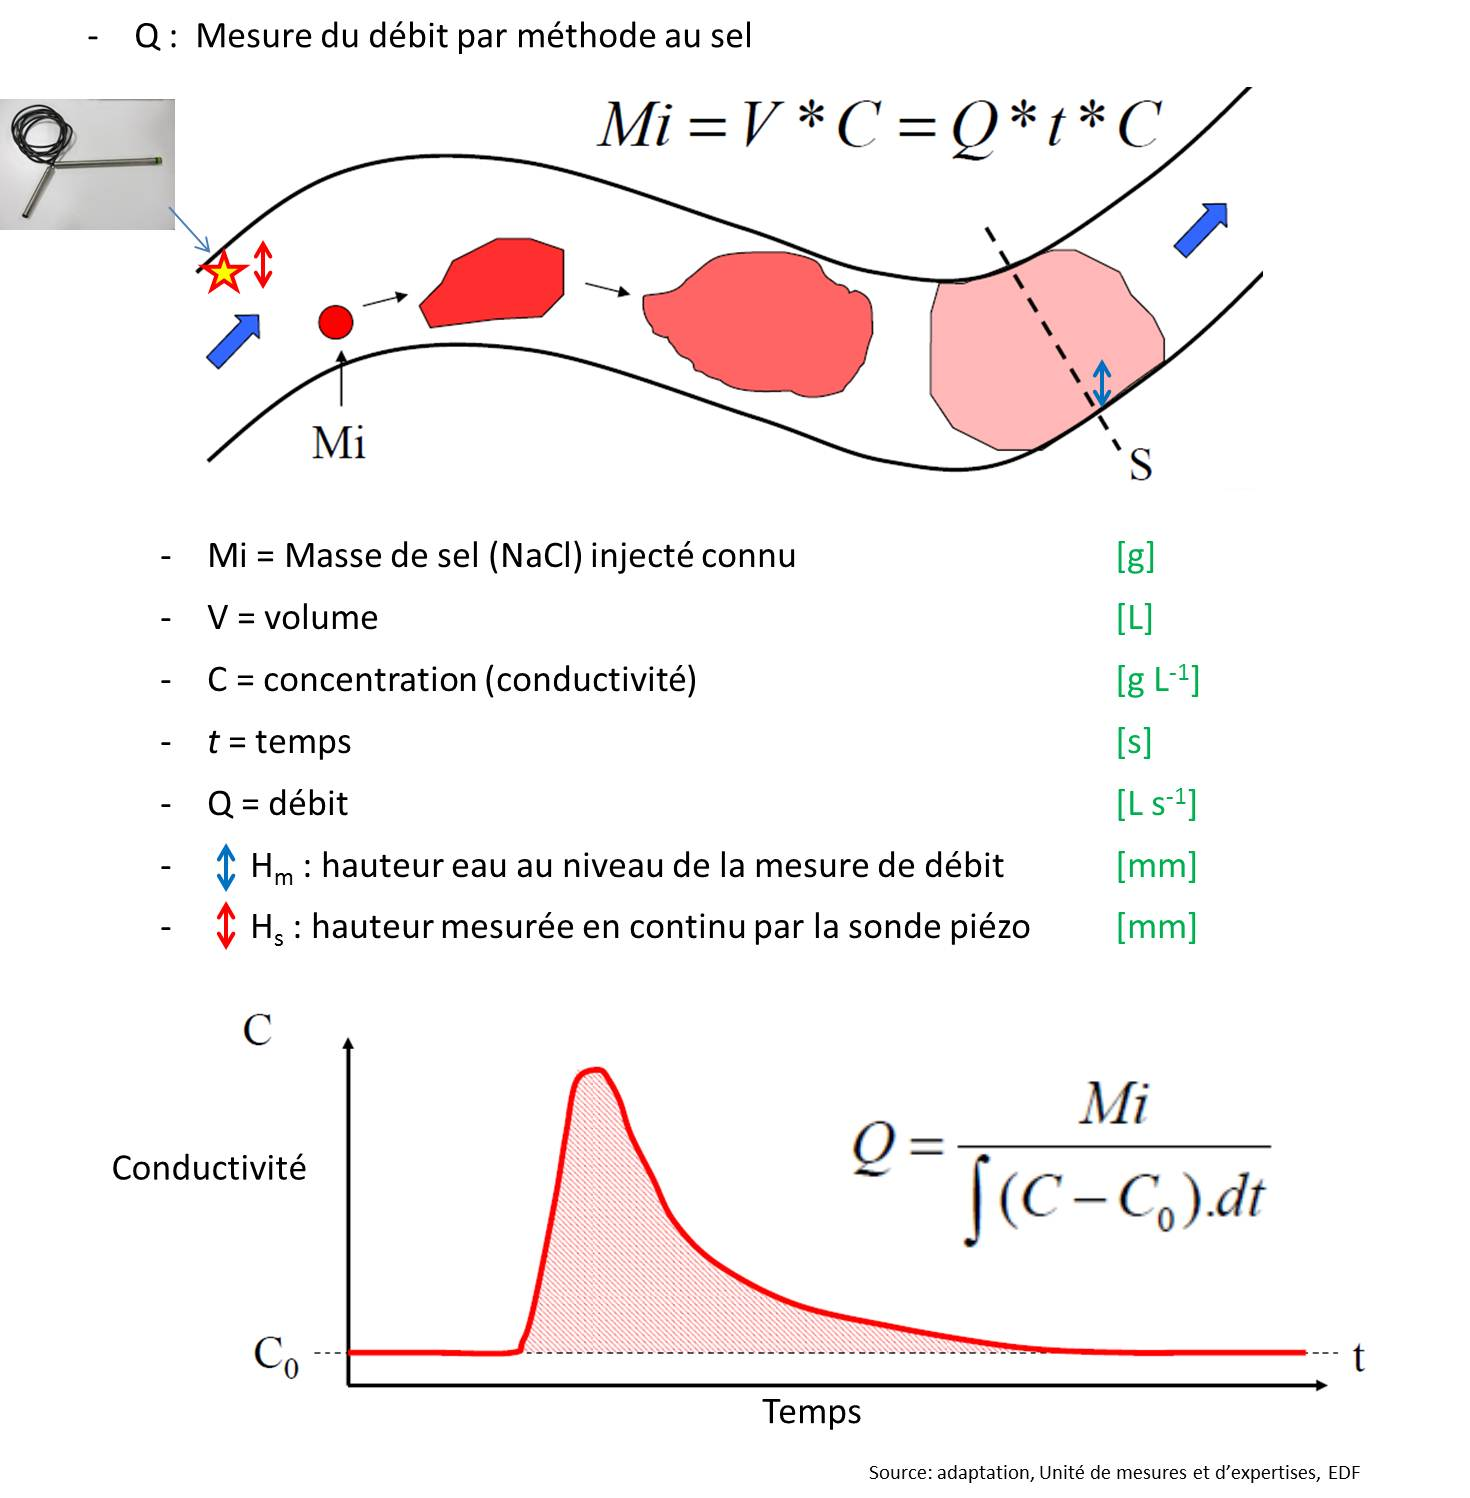
\includegraphics[width=11cm]{hydro_3.jpg}
		\caption{Sch�ma des mesures du d�bit au sel.}
		\label{Fig. hydro 2}
	\end{figure}
	
A partir du d�bit mesur� avec la m�thode au sel et la hauteur de la colonne d'eau � l'exutoire au moment de la mesure, il est possible de r�aliser une courbe de tarage (Fig. 4.3). La relation physique entre ces deux param�tres et sa repr�sentation math�matique sont connues. Il est alors possible de d�terminer les param�tres d'une fonction. En injectant les mesures � hautes fr�quences de hauteur de la colonne d'eau dans la fonction param�tr�e pr�c�demment (sp�cifique � chaque site), il sera possible d'obtenir des donn�es de d�bit Q � haute fr�quence (Fig. 4.3).

	\begin{figure}[h] 
		\centering
		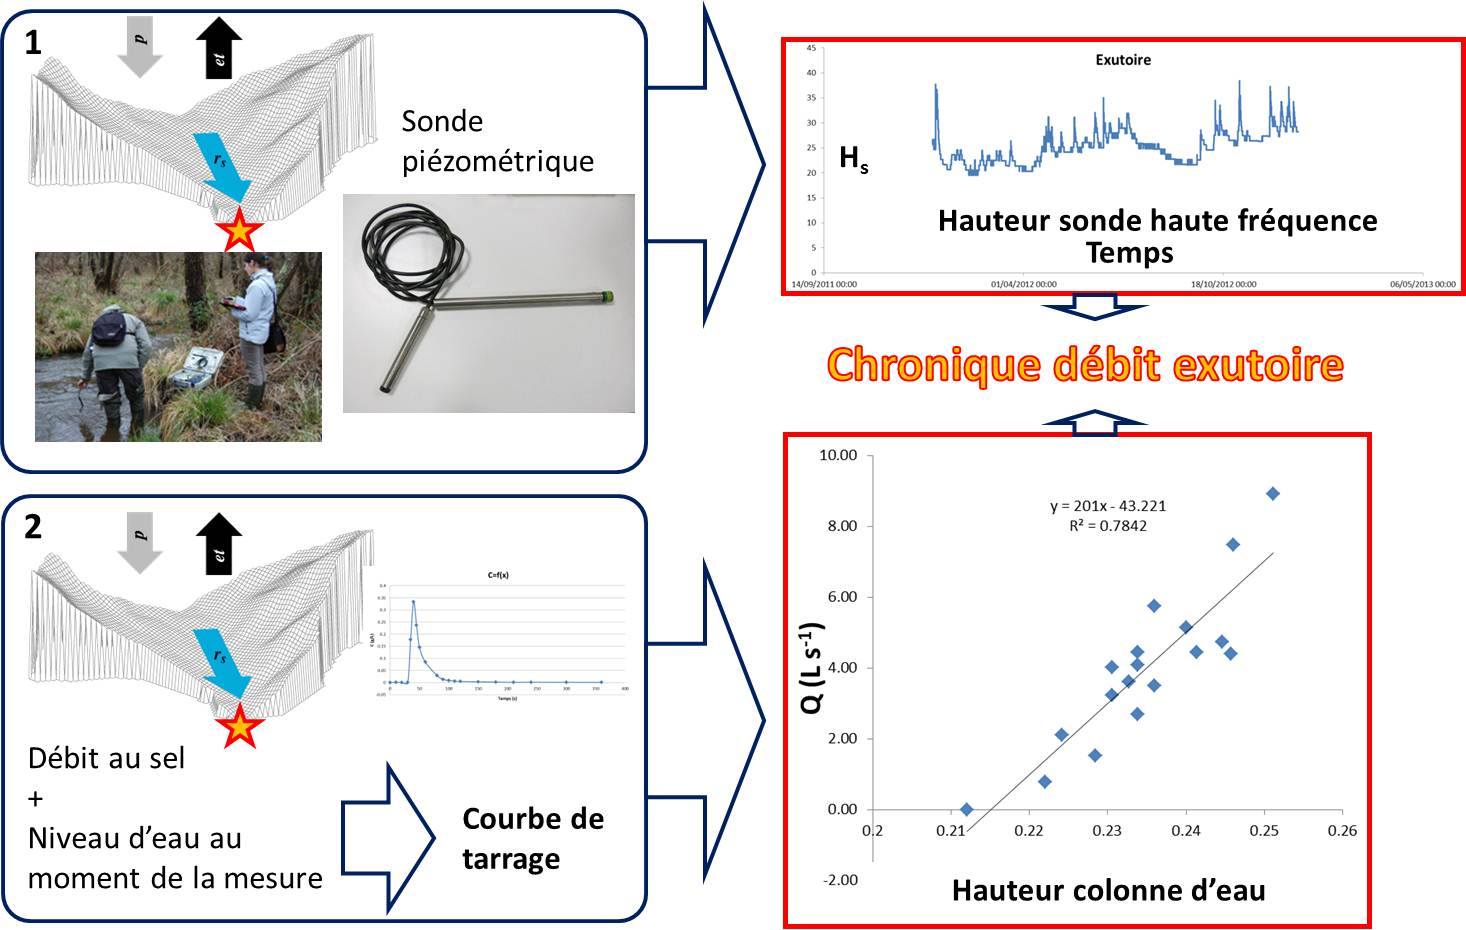
\includegraphics[width=11cm]{hydro_4.jpg}
		\caption{Calcul des chroniques de d�bit � partir des hauteur de la colonne d'eau � haute fr�quence et de la courbe de tarage.}
		\label{Fig. hydro 3}
	\end{figure}
	
Dans la base de donn�es, les donn�es en sortie de capteur (H) sont inject�es au moins une fois par an dans le dossier "fichiers annuels" des dossiers "data brutes" des diff�rents sites (cf section 2.3.2) par l'expert responsable de l'hydrologie de chaque site (cf flux de donn�es 2.3.1, cas 2). En plus des donn�es � hautes fr�quences des hauteurs d'eau, un fichier contenant les r�sultats de la courbe de tarage sera plac� �galement dans les fichiers de donn�es brutes au moins une fois par an. Ces fichiers auront pour nom : "FR\_xxx\_tarage\_yy", avec xxx pour le code du site et yy pour l'ann�e de mesure. Le nom des lignes devra se conformer au format d�crit au chapitre 1. Les donn�es de d�bit � l'�xutoire (Q) sont plac�es dans le dossier "fichiers annuels" des dossiers "data corrig�es" des diff�rents sites (cf section 2.3.2). Les actions r�alis�es sur les donn�es brutes sont consign�es dans le log correspondant. Le nom des fichiers sera bas� sur la nomenclature d�crite au chapitre 1. Le num�ro de la station pour la variable GWL permettra de savoir s'il s'agit de donn�es provenant de l'int�rieur de la tourbi�re o� de son exutoire.

\newpage

		
\newpage

		%--- CHAPITRE 5:Flux de C par Eddy-covariance
		
%------------------ %   Chapitre 5   %----------------- %


% % % % % % % % % % % % % % % % % % % % % % % % % % % % % 
%														%	
%			 SNO Tourbi�res - Eddy covariance			%
%														%	
% % % % % % % % % % % % % % % % % % % % % % % % % % % % % 





\chapter{Mesures de flux de carbone par eddy-covariance}

S. Gogo

\section{Cadre et objectif des mesures}

	
\newpage

\section{Organisation des �quipements}

\subsection{Nombre de station d'acquisition}

\subsection{installation des stations}


\newpage


\section{Les variables: mesures, nomenclature, et capteurs}

\subsection{Nombre et fr�quence}

\subsection{Nomenclature et codes}


\newpage


\section{Mesures de la vitesse et direction du vent en 3D}

\subsection{Principe de mesure et unit�}

\subsection{Positionnement du capteur}

%\subsection{Maintenance du capteur}

\subsection{Calibration et d�rive du capteur}


\newpage


\section{Mesure des flux de CO$_{2}$}

\subsection{Principe de mesure et unit�}

\subsection{Positionnement du capteur}

%\subsection{Maintenance du capteur}

\subsection{Calibration et d�rive du capteur}



\newpage


\section{Mesure des flux de CH$_{4}$}

\subsection{Principe de mesure et unit�}

\subsection{Positionnement du capteur}

%\subsection{Maintenance du capteur}

\subsection{Calibration et d�rive du capteur}

\newpage

\section{Mesure des flux d'H$_{2}$O}

\subsection{Principe de mesure et unit�}

\subsection{Positionnement du capteur}

%\subsection{Maintenance du capteur}

\subsection{Calibration et d�rive du capteur}
%La qualit� des donn�es peut �tre suivie en analysant les tendances du signal absolu du SWin, de l'albedo, de la corr�lation entre SW$_{in}$ et LW$_{in}$, SW pendant la nuit, et la corr�lation entre LW$_{out}$ et la temp�rature de surface. 


\newpage


\section{Maintenance de la station}
	\subsection{LI-7200RS (CO$_2$ et H$_2$O)}
		\subsubsection{Toutes les 2 semaines}
		
En th�orie (manuel d'utilisation), certaines des actions de cette section devraient �tre r�alis�es � une fr�quence plus �lev�e (une fois par jour ou quelques jours, toute les semaines). Comptes tenu de la distance des sites, ces actions de maintenance seront r�alis�es au moins toute les 2 semaines (en d�but de mesures en tout cas).

\

V�rifier les performances de l'instrument en v�rifiant les valeurs mesur�es:

\begin{itemize}
\item Temp�rature de l'air
\item Pression
\item Temp�rature sonic
\item Point de ros�e
\item Concentrations des gaz
\item Covariances et flux
\end{itemize}

\

V�rifier les performances de l'instrument en v�rifiant les informations diagnostiques:

\begin{itemize}
\item Force du signal
\item Temp�rature du d�tecteur
\item Temp�rature du bo�tier du chopper
\item Thermocouples
\end{itemize}

\
 
Si une baisse de la force du signal est observ�e, l'optique doit �tre nettoy�e (voir paragraphe nettoyage du parcours optique ci-dessous). La fr�quence de cette action d�pend de l'environnement de mesure. Dans le cas de nos sites de tourbi�res (air relativement pur), cette fr�quence devrait �tre basse (mais reste � d�finir avec la pratique et peut varier d'un site � l'autre).

En fonction des conditions du milieu, le filtre situ� juste apr�s l'entr�e d'air peut se boucher assez rapidement. Ce filtre est de type Swagelok FW-2 (enti�rement en acier inoxydable). Il peut �tre r�utilis� et nettoy� plusieurs fois (voir paragraphe nettoyage du filtre Swagelook FW-2 ci-dessous).


		\subsubsection{Chaque mois}

\begin{itemize}
\item V�rifier le z�ro
\item Faire un point de calibration et noter la valeur du \textit{S$_c$}
\item T�l�charger les donn�es
\item V�rifier les cables (dommages, serrage des colliers)
\item V�rifier les tubes (dommages, noeud)
\end{itemize}

Avec l'exp�rience, la fr�quence de la r�alisation du z�ro et du point de calibration pourra �tre ajust�e.

		\subsubsection{Chaque 6 mois}

Si l'instrument est dans un environnement humides, il faut remplacer les produits chimiques se trouvant dans l'analyseur (� verifier avec Licor si cela doit �tre effectivement fait � cette fr�quence).

		\subsubsection{Chaque ann�e}

Remplacer les produits chimiques se trouvant dans l'analyseur si cela n'a pas �t� fait tous les 6 mois.

Nettoyer/remplacer les filtres si n�cessaire.

		\subsubsection{Tous les 2 ans}

V�rifier la calibration avec au moins gaz de calibration suppl�mentaire et/ou retourner l'appareil chez Licor pour chack complet (� v�rifier, mais je crois que cette derni�re action est obligatoire dans ICOS).

		\subsubsection{Nettoyage du parcours optique}

Le parcours optique doit �tre nettoy� r�guli�rement en fonction des caract�ristiques de l'environnement de mesures. Pour ce faire, le banc optique doit �tre ouvert en d�vissant les 2 vis se trouvant sur la t�te du capteur et en la tirant vers le haut (Fig. 5.1). Le banc optique peut ainsi �tre retir� (removable optical bench sur la Fig. 5.1). Les fen�tes optiques (optical windows sur Fig. 5.1) peuvent �tre nettoy�es avec du d�tergent doux ou du lave-glace avec un chiffon de nettoyage sans peluche. Le banc optique peut �tre lav� avec du savon doux et de l'eau. Le banc optique est constitu� d'un insert en PVC. Par cons�quent, il ne faut \textbf{jamais utiliser d'ac�tone, de l'eau de javel ou une brosse m�tallique pour nettoyer le banc optique.}

	\begin{figure}[h] 
		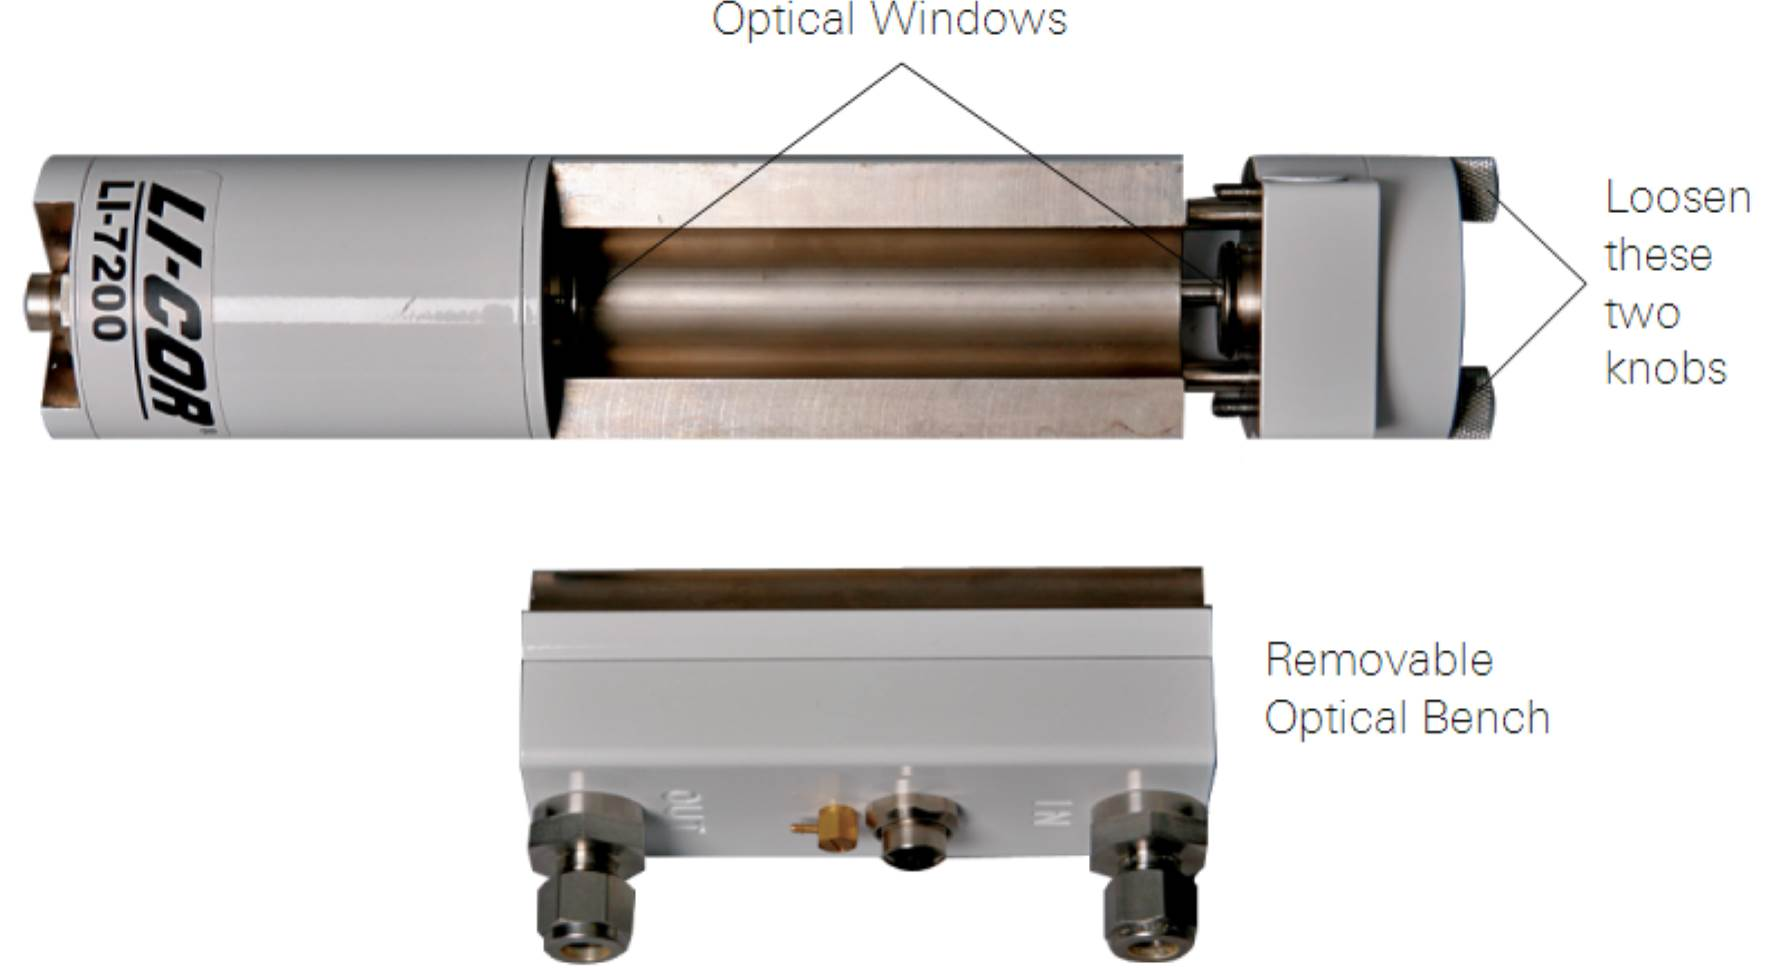
\includegraphics[width=12cm]{LI7200RS_1.jpg}
		\caption{Faire glisser la t�te du capteur (partie � droite de la photo) pour permettre de sortir le banc optique.}
		\label{Fig.1}
	\end{figure}
	
	
		\subsubsection{nettoyage du filtre Swagelook FW-2}

	\begin{itemize}
		\item utiliser de l'air comprim� filtr� (300 kPa, air grade z�ro ou azote ultre pure) pour souffler les particules les plus grandes dans la direction inverse du flux d'air
		
		\
		
		\item placer le filtre dans un bain a ultrasons pendant 2 heures avec du d�tergent de laboratoire dilu� dans le l'eau d�ionis�e ou ultra-pure
		
		\
		
		\item rincer avec de l'eau distill�e dans le sens oppos� du flux d'air, puis dans le sens du flux d'air
		
		\
		
		\item utiliser de l'air comprim� filtr� (200 kPa, air grade z�ro ou azote ultre pure) pour souffler les particules les plus grandes dans la direction inverse du flux d'air, puis dans le sens du flux d'air
		
		\
		
		\item rincer une nouvelle fois aux ultrasons avec de l'eau distill�e pendant une heure et souffler � l'air comprim� (300 kPa) dans la direction inverse du flux d'air, puis dans le sens du flux d'air
		
		\
		
		\item laisser s�cher pendant 24h dans un endroit propre et sec
		
		\
		
		\item inspecter visuellement l'entr�e et la sortie du filtre pour d�tecter toute trace de corrosion (si corrosion, remplacer le filtre)
	\end{itemize}


		\subsubsection{Fusible}

L'alimentation du LI7200RS est prot�g� par un fusible localis� en bas � gauche dans le boitier. Le remplacer si n�cessaire (5A fast blow, 125V, 5x20mm; #439-04214).

		\subsubsection{Remplacement des thermocouples}
		
Des thermocouples avec un fil fin sont localis�s � l'entr�e et � la sortie de l'air. Ils mesurent la temp�rature de l'air entrant et sortant. S'ils sont cass�s, il faut les remplacer de la mani�re suivante:

\begin{itemize}
\item D�gager le banc optique comme d�crit pr�c�demment
\item Utiliser une cl� Allen 7/64 pour enlever les 8 vis du banc optique (Fig. 5.2)
\item Enlever le l'ensemble portant le thermocouple (Fig. 5.3)
\item Mettre un nouveau thermocouple en faisant attention 1) � bien mettre les broches de connections et 2) � ce que les 2 joints toriques soient bien en place
\item Remonter le tout
\end{itemize}


	\begin{figure}[h] 
		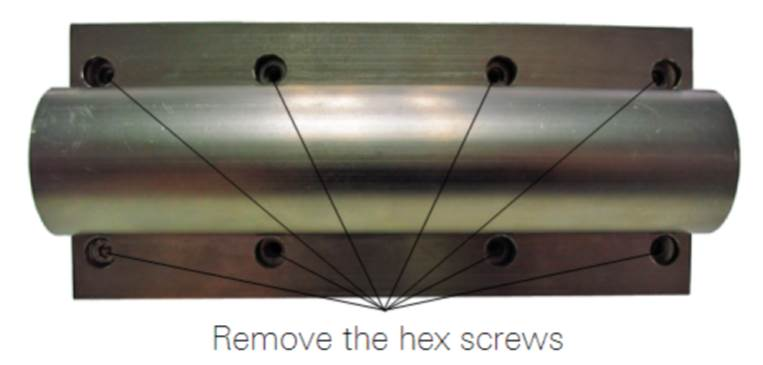
\includegraphics[width=12cm]{LI7200RS_2.jpg}
		\caption{Faire glisser la t�te du capteur (partie � droite de la photo) pour permettre de sortir le banc optique.}
		\label{Fig.1}
	\end{figure}


	\begin{figure}[h] 
		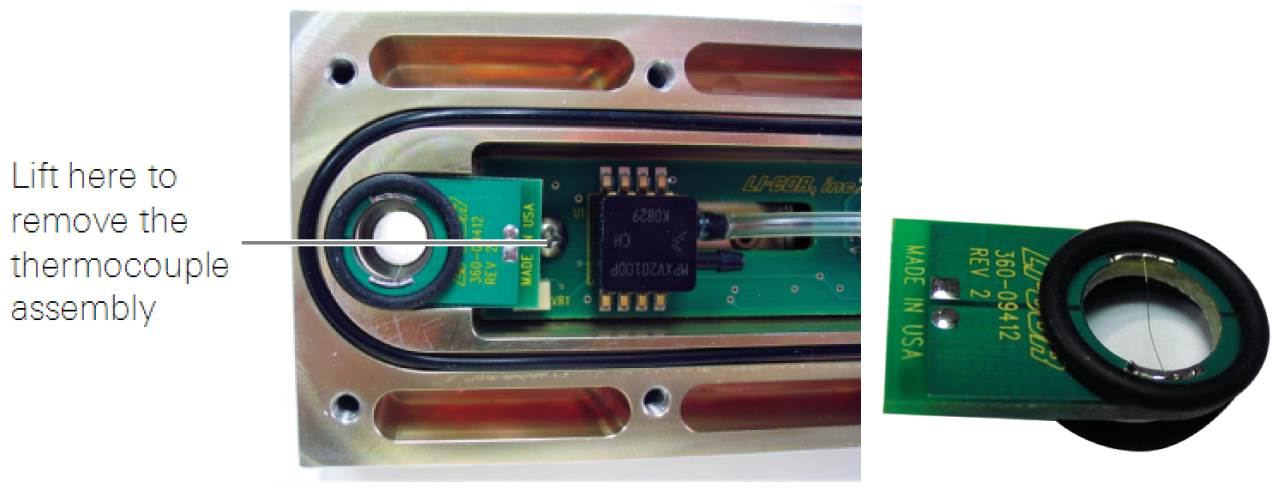
\includegraphics[width=12cm]{LI7200RS_3.jpg}
		\caption{Faire glisser la t�te du capteur (partie � droite de la photo) pour permettre de sortir le banc optique.}
		\label{Fig.1}
	\end{figure}




		\subsubsection{Nettoyer la prise d'air et le filtre}

Apr�s avoir d�monter l'�l�ment au bout du tube assurant la prise de l'�chantillon d'air (Fig. 5.4), soufflez dedans ou passez de l'eau. L'embout peut �tre laver dans de l'eau bouillante ou aux ultrasons. Le filtre (screen sur le Fig. 5.4) n'a pas vocation a �tre retir� pendant le nettoyage. Si cependant, il doit �tre enlev�, la faire avec petit tournevis avec beaucoup de pr�caution pour ne pas endommager l'embout

Plus le filtre sera rempli de poussi�re, plus le module de flux va utiliser d'�nergie. Par cons�quent, le meilleur indicateur d'un filtre bouch� est un changement du besoin d'�lectricit�. En cas de changement du filtre, notez le flux (en \%). Avec le temps, comparez cette valeur avec la valeur initiale. \textbf{Il faut laver le filtre avant que le flux d�passe 90 \%}. Le filtre peut �tre lav� dans un bain d'eau avec des ultrasons, souffl� ensuite avec de l'air comprim�


	\subsection{LI-7700 (CH$_4$)}

		\subsubsection{Changement du dessicant}

Le dessicant se trouvant dans l'�l�ment sup�rieur du LI700 doit �tre chang� une fois par an. Ceci peut �tre v�rifi� dans le cadre "Calibration" de la fen�tre principale, o� la valeur "Optics RH" doit �tre autour de z�ro. Si l'indicateur est rouge, quand la valeur d'"Optics RH" est sup�rieure � 30 \%,  le dessicant doit �tre chang�.

		\subsubsection{Les miroirs}
		
Bien que les miroirs sup�rieur et inf�rieur soient tr�s r�sistant, il est pr�f�rable de les traiter comme des optiques sensibles. Ne pas mettre trop de pression lors du nettoyage des miroirs. S'ils sont couvert de poussi�res, laver les miroirs avec un chiffon propre mouill� avec de l'eau ou un liquide lave vitre. Le r�servoir pour le lavage automatique peut �tre rempli de liquide pour pare-brises. Si l'encrassement est faible, de l'eau du robinet peut suffire.

		\subsubsection{Thermocouples}
Si n�cessaire, changez le thermocouple (#9977-038) comme suit:
		
\begin{itemize}
\item D�connecter l'alimentation pour �teindre le LI7700
\item d�viser les 2 vis dans la partie sup�rieur qui maintiennent le thermocouple
\item R�cup�rer le thermocouple
\item Mettre le nouveau sans forcer et en s'assurant que la pointe est dirig�e vers l'int�rieur de la cellule de mesure
\item Remettre les vis, remettre, l'alimentation connecter le LI7700 et v�rifier la mesure de temp�rature
\end{itemize}


		\subsubsection{Le fusible}

Idem section pr�c�dente (5A fast blow, 125V, 5x20mm; #439-04214)


	\subsection{LI-7200-101 (module de flux pour le LI7200)}


		\subsubsection{Le fusible}
		
Pour changer le fusible, d�visez le capuchon et le remplacer (5A fast blow, 125V, 5x20mm; #439-04214).

		\subsubsection{Le filtre}
		
Plus le filtre sera sale, plus le module aura besoin d'�nergie pour maintenir le bon flux d'air. Le filtre peut �tre chang� (301-10382) ou lav� avec de l'eau ou de l'air comprim�.
		

		
\newpage

		%--- CHAPITRE 6: Flux de C avec chambre d'accumilation
		%\include{protocole_6_chambre}

\newpage

		%--- CHAPITRE 7: V�g�tation
		%\include{protocole_7_vegetation}

\newpage

		%--- CHAPITRE 8: Biog�ochimie
		%\include{protocole_8_biogeochimie}

\newpage

		%--- CHAPITRE 9: Glossaire
		\include{protocole_9_glossaire}
		
\newpage

		%--- CHAPITRE 10: Glossaire
		%\include{protocole_10_maintenance}


\end{document}